\chapter{Optimal Dynamic Selection of Gear-ratios}  % to exploit or attenuate the external load dynamics
\label{sec:ControlAndPlanningOfRobotUsingVariableGearRatioActuators}

%\begin{flushright}
%\textit{"With four parameters I can fit an elephant, and with five I can make him wiggle his trunk."} \\ \emph{John von Neumann}
%\end{flushright}

\begin{flushright}
\textit{"He will win who knows when to fight and when not to fight."} \\ \emph{-- Sun Tzu}
\end{flushright}
\vspace{10pt}

The transmission gear-ratio that couples an actuator to a load has a significant effect on the behavior of the actuator-load system. With a large reduction ratio, the load-side dynamics has no significant effect because it is attenuated by the factor of the square of the gear-ratio. The net load acting on the actuator is mostly its own intrinsic load, including rotor inertia and friction. In contrast, with a small reduction ratio or a direct drive system \cite{asada_direct-drive_1987}, the behavior is usually dominated by the load-side dynamics which consist of highly non-linear inertial and gravitational forces for robotics manipulators. Sometime it can be advantageous to exploit the load-side dynamics: gravity may push the robot in a desired direction; the robot may coast with small dissipative torques induced at the actuator side; or the robot joints become backdrivable to comply to an external force. In other situations, however, it may be advantageous to isolate the actuators from the load-side dynamics and external disturbances: using a large gear-ratio to bear a large load or moving it slowly against gravity, for example.

This chapter aims to explore the potentials of actuator transmissions that can be switched dynamically, such as the technology presented in chapter \ref{sec:MultipleSpeedActuationTechnology}, to either attenuate or leverage the natural dynamics of the system. Robots using lightweight VGA have the potential for achieving fast motions, high load-bearing, compliance and high-impedance, as required by diverse load conditions encountered by robotic systems. However, to truly exploit those salient features of VGA, control laws to select dynamically gear-ratios based on the current situation and task of the robot must be developed. Here in this chapter, feedback laws for robot control including gear-ratios selection are thus explored. The variable gear-ratios are used not merely for increasing maximum torque and speed, but also to significantly alter the dynamic properties, including load sensitivity, robustness, and backdrivability, advantageously given the situation.

%Outline
In section \ref{sec:princ}, the principle of load leveraging and attenuation is delineated for a simple 1-DoF manipulator. Section \ref{sec:chal} discuss related works and technical challenges and section \ref{sec:maincont} details the main original contributions. Section \ref{sec:model} introduces a formal mathematical representation and propose a dynamic model for robotic systems using VGA. Two different control approaches are explored, a model-based control laws synthesis in section \ref{sec:HierachicalControlApproach}, and a computational approach in section \ref{sec:DynamicProgrammingAproach}. The advantage of actively changing the gear-ratios are then illustrated with simulations in section \ref{sec:shift_sim}, and with experiments using a robotic arm using custom-built variable gear-ratio actuators in section \ref{sec:shift_exp}.

\subsection{Illustration of the principle for a 1-DoF manipulator}
\label{sec:princ}

Fig. \ref{fig:bigpicture} illustrates a simplified 1-DoF robotic manipulator where an electric motor is coupled to a pendulum through a gearbox with a gear-ratio $R$.
%
\begin{figure}[ht]
 %\vspace{-10pt}
	\centering
		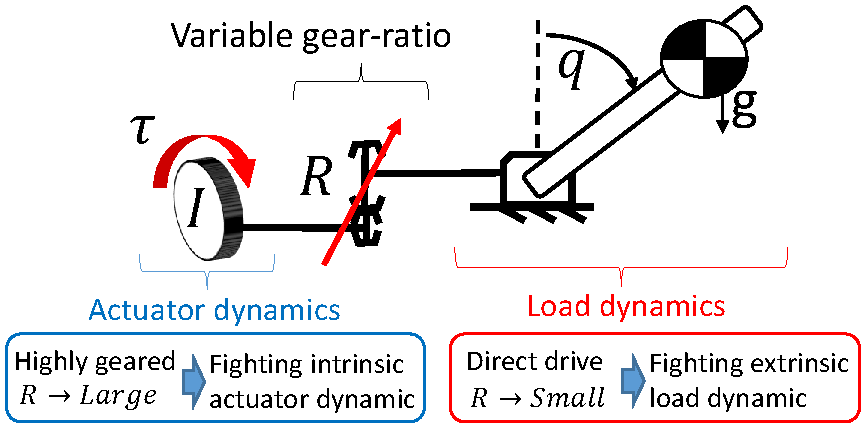
\includegraphics[width=0.75\textwidth]{gearratioeffect.pdf}
	\caption{Effect of the gear ratio on the dynamics}
	%\vspace{-10pt}
	\label{fig:bigpicture}
\end{figure}
%
As illustrated by phase portraits in Fig. \ref{fig:pp}, if $R$ is small then the dynamic behavior of the system is dominated by the non-linear pendulum dynamics (Fig. \ref{fig:pp1}), but if $R$ is very large, the behavior is dominated by the intrinsic inertia of the actuator, leading to the double-integrator behavior (Fig. \ref{fig:pp2}).
%
\begin{figure}[ht]
				%\vspace{-10pt}
        \centering
				\subfloat[ Reduction ratio $R$=1 ]{ %extrinsic dynamics
				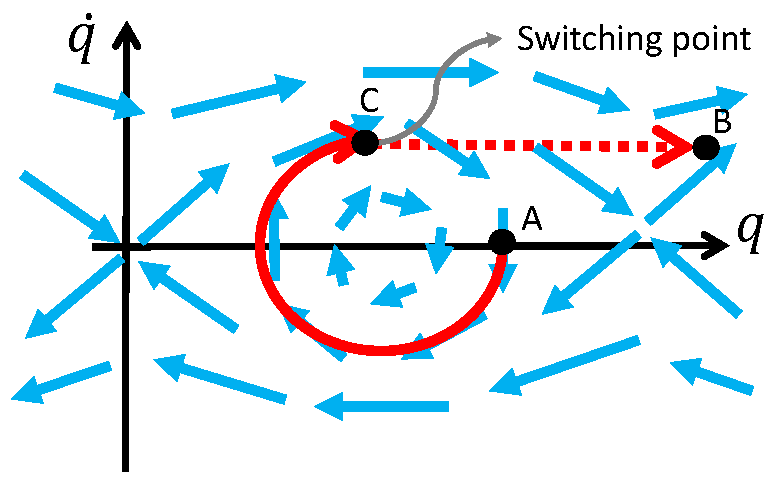
\includegraphics[width=0.40\textwidth]{pp1_hand.pdf}
				\label{fig:pp1}}
        \subfloat[Reduction ratio $R$=10 ]{ % intrinsic dynamics
				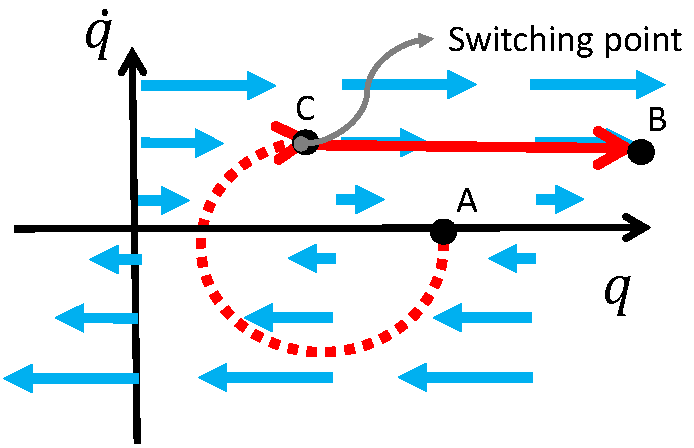
\includegraphics[width=0.40\textwidth]{pp10_hand.pdf}
				\label{fig:pp2}}
        \caption{Phase portraits illustrating the dynamical behavior}
				\label{fig:pp}
\end{figure}

The vector fields of Fig. \ref{fig:pp} illustrates the natural evolution of the system with no actuator torques. Suppose that we want to move from state A to state B on the phase plane. Starting off state A with the gear-ratio of 1:1 brings the system along the curved trajectory shown in Fig. \ref{fig:pp1}. Switching the gear-ratio to 1:10 at state C will change the trajectory to the one in Fig. \ref{fig:pp2}, and bring the system to the destination state B. Note that no actuator torque is necessary for following this trajectory. A salient feature of actively changing the gear-ratio is that, the natural vector field behavior can be altered, in order to move in the desired direction with small torques.

%a vector field having properties useful for moving in a desired direction can be selected to minimize the necessary torque to apply to the system. 


\subsection{Challenges and related works}
\label{sec:chal}

This chapter investigates closed-loop control scheme for robots equipped with variable gear-ratios actuators. While variable transmissions have been studied extensively for automobile power-trains, they have not yet been fully investigated in robotics, despite significant potential gains. Variable gear-ratio transmissions for electric motors have been proposed for legged locomotion \cite{hirose_design_1991}, grasping robotic hands \cite{shin_robot_2012} , propulsion system \cite{lee_new_2012} \cite{mckeegan_antonovs_2011} and actuation systems \cite{girard_two-speed_2015} \cite{hirose_development_1999} \cite{tahara_high-backdrivable_2011}. Some of those works address the issue of how to change the gear-ratio, but there is no general approach to the high-level control of automatically selecting the right gear-ratios for non-linear, coupled multi-DoF robotic systems.

From the control perspective, automating the gear-ratios selection in a robotic context is a new and challenging problem. Gear-shifting is a very non-linear process (gear-ratios variables multiply other inputs and states in the equations of motion) and moreover the plant becomes a hybrid dynamical system if the usable gear-ratios are a set of discrete values. Hence most control engineering tools are not suited to tackle this problem. In simple scenarios, the gear-ratio selection can be based on simple principles. For instance, for a system running at a steady speed and load, the best gear-ratio can be selected based on efficiency maps. Alternatively, for rapid acceleration, the gear-ratios may be selected based on the actuator-load inertia matching \cite{giberti_effects_2010} \cite{chen_generalized_1991}. A robot, however, experiences diverse types of forces acting simultaneously. These include gravity, friction, and inertial forces as well as Coriolis and centrifugal forces. Hence, it is challenging to find a general control policy for selecting gear-ratios for the multitude of dynamically interacting actuators in the robotics context. 

\paragraph{Trajectory planning}

In robotic, the generation of good reference trajectories is usually formulated as an optimization problem. Most optimal control techniques are based on either variational approaches or some form of gradient descent to find a trajectory that minimizes a cost function \cite{betts_practical_2010}. Hence those techniques cannot be used directly to optimize discrete variables. An interesting approach to get around this problem is to use the switching instants as optimization parameters instead \cite{xu_optimal_2004}\cite{majdoub_hybrid_2010}. However, to use this approach a sequence of operating modes must be predefined first. Mixed-integer programming can be used to generate optimal open-loop trajectories of dynamical system with both continuous and discrete input variables \cite{richards_spacecraft_2002}. For instance, mixed-integer programming has been used to generate optimal open-loop trajectories for a car with both a continuous torque and a discrete gear-selection input \cite{gerdts_solving_2005}. Computation time was however in the order of hours for a 6 sec trajectory. 

Sample-based planning scheme can also be used to find efficient trajectory \cite{lavalle_planning_2006}. These algorithms work generally better then optimization approaches when tackling highly-constrained system and when the goal is only to find a feasible trajectory and not necessary the optimal solution. The other advantage is that discrete control actions, like the selection of a gear-ratio in a discrete set, can be considered without complications since these algorithm works with discretized models.

Open-loop trajectories can be unstable and if the system deviates from the original plan, due to uncertainty, the optimized gear-ratios sequence might be completely un-adapted after some time. For a robotic system to really leverage the advantage offered by multiple gear-ratios, it would be advantageous if gear-ratios are selected actively based on the actual conditions of the system. This chapter focuses on finding closed-loop policies for the gear-ratios selection.

\paragraph{Feedback control}

One possible approach for closing the loop would be simply to re-plan trajectory continuously online. However, the rate at which this would be possible for hybrid robotic systems would not be sufficient. Here we aim at having control policies that can react to a situation in a matter of milliseconds, for instance down-shifting as a robotic leg touch the ground. Most of the analytical results regarding feedback control of hybrid systems are for specific cases, for instance the optimal feedback laws for linear hybrid systems with linear constraints and a quadratic cost function have been shown to have a particular form \cite{borrelli_dynamic_2005}. One computational technique that generate feedback laws and that can be used for non-linear systems with any kind of constraints is dynamic programming \cite{kirk_optimal_2004}. Two disadvantages of the techniques are however that it is only computationally tractable for low-dimensional systems (so called curse of dimensionality) and also that the resulting feedback laws are in the form of a look-up table. This approach is investigated in section \ref{sec:DynamicProgrammingAproach}, which is an extension of work published by the author in \cite{girard_practical_2016}.

\subsection{Original contributions}
\label{sec:maincont}

The main original contribution of this chapter, is an alternative model-based approach (section \ref{sec:HierachicalControlApproach}) with the advantage of scaling to high-dimensional robotics system, and easily applicable to trajectory tracking problems. The main idea was introduced by the author in \cite{girard_leveraging_2017} and this thesis chapter presents improved algorithms and new results. The main ideas to make tractable closed-loop control of this type of multi-DoF non-linear hybrid systems are 1) Using a simple modeling approach for variable transmissions that does not augment the number of state variables. 2) Exploiting the structure in the equations of motion when expressed in the inverse-dynamic form.  3) Using an outer-loop first specifying an instantaneously desired acceleration $\ddot{\vec{q}}_r$, similarly to feedback linearization, which fix locally the trajectory and makes possible computation of optimal instantaneous gear-ratios.

To the best knowledge of the author, this is the first exploration of closed-loop selection of gear-ratios for multi-DoF robotic systems. Many conceptual insight regarding gear-ratios selection when fighting different type of forces and unknown disturbances are explored. The treatment also encompass the very wide class of $n$-DoF mechanical system with EoM that can take the form of so-called manipulator equations (eq. \eqref{eq:manipulator}, and is valid for many type of variable transmissions. The main restriction is that each joint of the system must be actuated, although it could also be extended to under-actuated systems when using a partial feedback linearization approach. 


\newpage

\section{Control architecture}
\label{sec:arch}

This chapter proposed control schemes to dynamically select the optimal gear-ratios online. The focus is on feedback policies that can react quickly to the states of the robot, and engage the appropriate gear-ratios with minimal delays (in the order of 20 msec). Two approaches are investigated and illustrated at Fig. \ref{fig:controlarchitectures}. 
%
\begin{figure}[H]
				\vspace{-10pt}
        \centering
				\subfloat[ Dynamic programming approach ]{ % intrinsic dynamics
				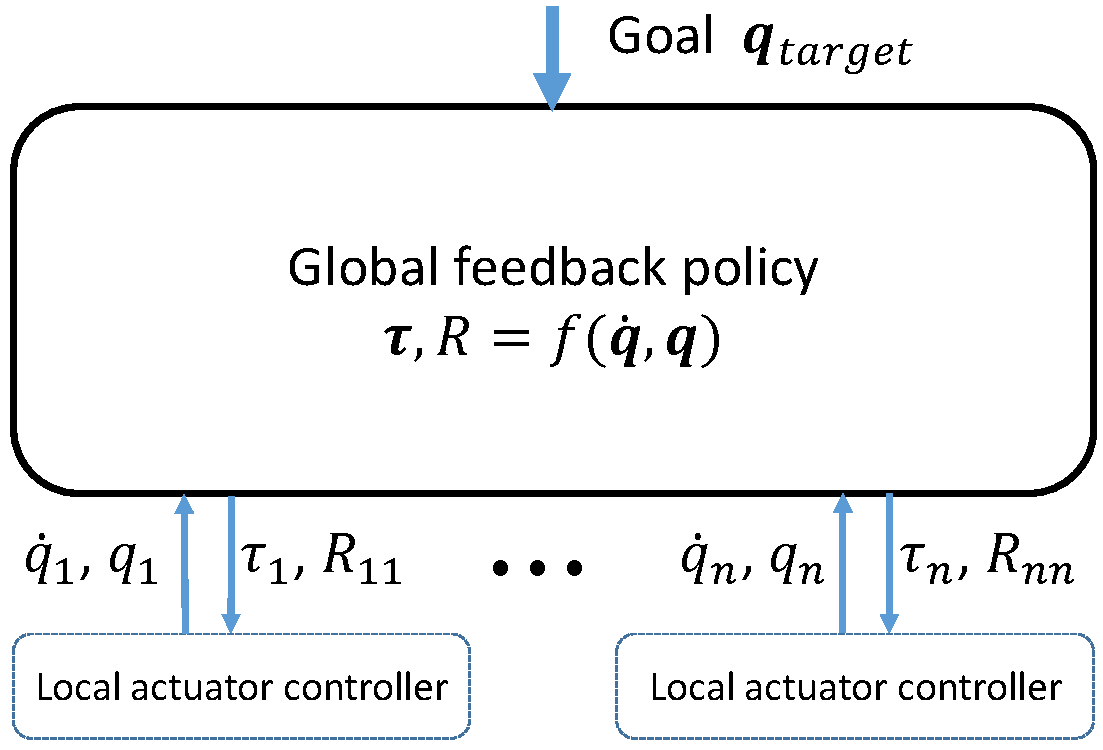
\includegraphics[width=0.45\textwidth]{archi2.pdf}
				\label{fig:archi2}}
				\hspace{+10pt}
				\subfloat[ Model-based approach ]{ %extrinsic dynamics
				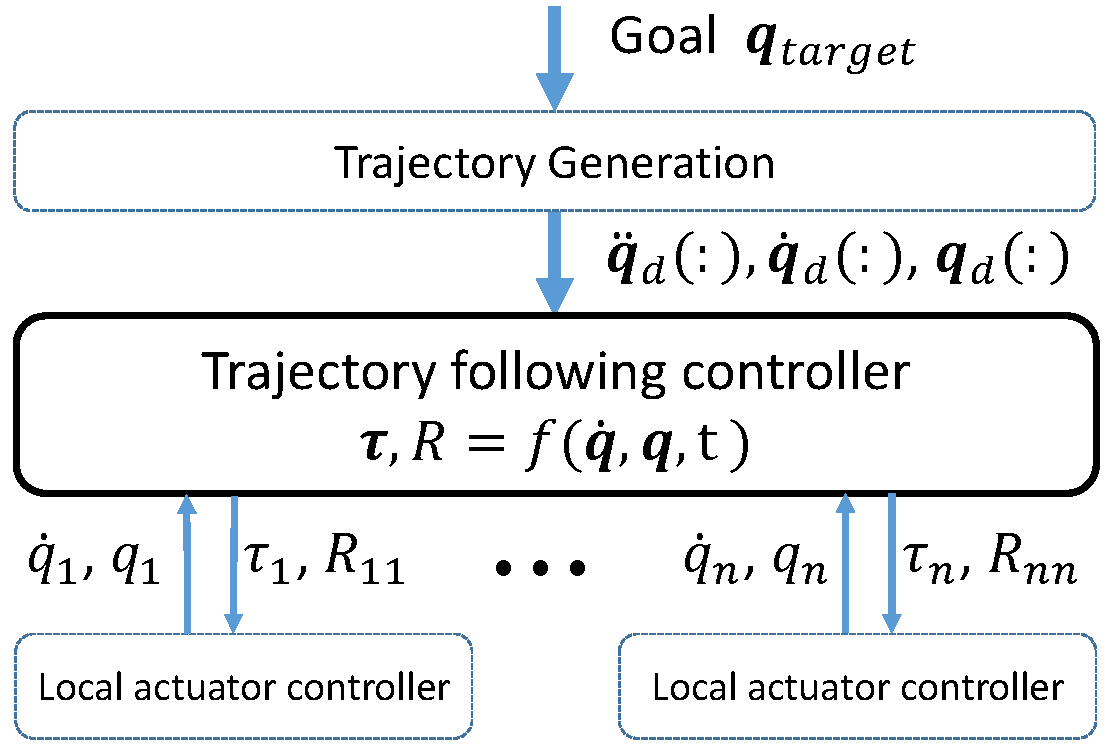
\includegraphics[width=0.45\textwidth]{archi3.pdf}
				\label{fig:archi3}}
        \caption{Proposed control architectures}
				\label{fig:controlarchitectures}
\end{figure}
%
The architecture of both control approaches is designed so the control signal is a torque and a gear-ratio for each actuator. Note that in the case of discrete gear-ratios options, instead of transmitting the actual gear-ratios $R$, the control signal can be a label $k$ indexing the discrete $R_k$ options. Hence, it is assumed that low-level VGA controllers handle tracking the motor torque setpoint and the gear-shifting process. This is analogous to automating a car equipped with a semi-automatic transmission, and designing control policies replacing the driver for which the two control inputs are a throttle level a and shift-up/shift-down signal. The low-level VGA controllers would be specific to the type of actuator used in the system. For the particular case where the VGA are DSDM actuators, the low-level controllers would be the control laws described in Chapter \ref{sec:MultipleSpeedActuationTechnology}. The architecture difference is that, for the dynamic programming approach given a goal, a global feedback policy is synthesized directly. However, for the model-based approach the high-level controller is separated into two levels. A feedback policy for trajectory tracking and an open-loop motion planning algorithm that generate a reference trajectory to reach the goal. 

\paragraph{Trajectory generation} Algorithm synthesizing a dynamic trajectory that meets performance requirements for reaching the target robot configuration starting at the actual robot configuration: 
%
\begin{align}
  \ddot{\vec{q}}_d(:),\dot{\vec{q}}_d(:),\vec{q}_d(:) = f_{planner}(\vec{q}_{target}, \vec{q})
	\label{eq:trajgen}
\end{align}
%
Computation time is in the order of 1-10 sec depending the robot complexity. Hence, this step is done offline in advance, or alternatively in closed-loop by re-planning continuously but at a very low rate. 

\paragraph{Low-level actuator controller} Independent actuator controllers executing low-level hardware commands in response to a torque and a gear-ratio set-points. For the particular case of a DSDM actuator the controller computes:
%
\begin{align}
  \tau_1 , \tau_2 , b_{state} = f_{DSDM}(\tau_i, R_{ii})
	\label{eq:low-level-dsdm}
\end{align}
%

\paragraph{Trajectory following controller} A function that compute torques and gear-ratios as a function of the robot actual states and the time:
%
\begin{align}
  \vec{\tau}, R = f_{ctl}(\dot{\vec{q}}, \vec{q} , t)
	\label{eq:trajctl}
\end{align}
%
 The function is synthesized based on a dynamic model of the robot and a desired trajectory. This function is to be executed in closed-loop at a high sampling-rate in the order of 1 kHz.

\paragraph{Global feedback policy} A function that compute torques and gear-ratios as a function of the robot actual states. This function is to be executed online in closed-loop at a high sampling-rate in the order of 1 kHz. However synthesis of the policy require a learning phase that require multiple hours of computation. 
%
\begin{align}
  \vec{\tau}, R = f_{ctl}(\dot{\vec{q}}, \vec{q})
	\label{eq:globctl}
\end{align}
%


%TODO incorporate this:

%The proposed control architecture, shown in Fig. XXX, consists of three hierarchical control loops. First, a trajectory generation algorithm synthesizing dynamic trajectories that meets performance requirements for reaching desired states. Second, a closed-loop trajectory following controller consisting of a feedback law computing actuator torques $\vec{\tau}$ and gear-ratios $R$ based on the measured full state of the robot. Finally at the lowest level, independent actuator controllers executing low-level hardware commands in response to given torques and gear-ratio set-points. 

%The main scope of this paper is the trajectory following controller: the design of a feedback law optimizing gear-ratios and computing torque commands in real-time. For the trajectory generation, motion planning algorithms can be applied to optimize the overall trajectory \cite{lavalle_planning_2006}.   It is assumed that they would track the desired torque/force and handle the gear-shifting process when receiving a new gear-ratio set-point. 


\newpage

\section{Modeling variable gear-ratio actuators}
\label{sec:model}

\begin{flushright}
{%\footnotesize %\small
\textit{"With four parameters I can fit an elephant, and with five \\ I can make him wiggle his trunk."}
 }
 \emph{-- John von Neumann}
\end{flushright}
\vspace{+10pt}

In this section, a simple approach is proposed for modeling robots using variable gear-ratio actuators. Variable transmissions are modeled as variable transformer elements, using the bond-graph terminology. This representation allows for a clear physical understanding of the effect of gear-ratios even for non-linear $n$-DoF systems. Furthermore, this modeling approach facilitates the implementation of a real-time optimization in the proposed controller. Limitations are discussed at section \ref{sec:limitation}.

%\begin{table}[htbp]
	%\centering
		%\begin{tabular}{ c c l }
		%
        %\hline \hline
			%$H$             &  :  & External inertia matrix \\
			%$D$             &  :  & External damping matrix \\
			%$C$             &  :  & External Coriolis/Centrifugal forces matrix  \\
			%$\vec{f}_g$     &  :  & External gravitational forces vector  \\
			%$\vec{d  }$     &  :  & External disturbances forces vector  \\
			%$R$             &  :  & Gear-ratio matrix (diagonal) \\
			%$I$             &  :  & Intrinsic actuator inertia matrix (diagonal) \\
			%$B$             &  :  & Intrinsic actuator damping matrix (diagonal) \\
			%$\vec{\tau}$    &  :  & Electromagnetic motor torques  \\
			%$\vec{q}$       &  :  & Joint coordinates position vector  \\
			%$\vec{w}$       &  :  & Actuator coordinates velocity vector  \\
			%$J$             &  :  & task-space coordinates / joint coordinates jacobian matrix\\
			%%&\text{Secondary variables:  \\
			%$\vec{f}$       &  :  & Net transmitted forces (joint coordinates) \\
			%$\vec{\tau}'$   &  :  & Net transmitted forces (actuators coordinates) \\
			%$\vec{\tau}_I$  &  :  & Sum of intrinsic forces  \\
			%$\vec{\tau}_E$  &  :  & Sum of extrinsic forces  \\
		%\hline \hline
        %\end{tabular}		
        %\caption{Nomenclature}	% Table caption must be placed on top of the table %
	%\label{tab:nom}
%\end{table}

\subsection{1-DoF system}
\label{sec:1DOFSystem}

First, a generic 1-DoF robot with a variable transmission is considered for simplicity. If the actuator's intrinsic resistive forces $\tau_I$ (rotor inertia and friction) are approximated to a linear quantity, the equations of motion (EoM) can be written as:
%
\begin{align}
  H \ddot{q} + D \dot{q} + g( q )	&= R  \left[ \tau - I \dot{w} - B w	\right] \\
	\underbrace{\left[	H \ddot{q} + D \dot{q} + g( q )	\right]}_{\tau_{E}(\ddot{q},\dot{q},q)}
	&= R \tau - R^2
	\underbrace{\left[ I \ddot{q} + B \dot{q}	\right]}_{\tau_{I}(\ddot{q},\dot{q})} \\
	\tau &= 	\frac{\tau_{E}(\ddot{q},\dot{q},q)}{R} + R \; \tau_{I}(\ddot{q},\dot{q})
	\label{eq:1dofEoM}
\end{align}
%
where the effect of the gear ratio can be seen clearly; increasing $R$ attenuates the external dynamic terms $\tau_{E}$ but amplify the intrinsic actuator losses $\tau_{I}$ for a given trajectory.
%
Variable gear-ratios can be modeled as variable transformer elements, using the bond-graph terminology. Fig. \ref{fig:bondgraph1} shows a bond-graph representation.
%
\begin{figure}[htp]
	\centering
		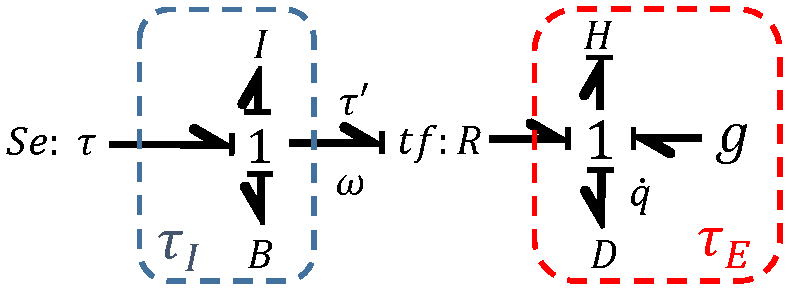
\includegraphics[width=0.50\textwidth]{bondgraph1.pdf}
	\caption{Model of a 1-DoF robot with a variable gear-ratio actuator}
	\label{fig:bondgraph1}
\end{figure}


\subsection{Generalization to n-DoF manipulators}
\label{sec:GeneralizationToNDOFManipulators}

To generalize the above model to a $n$-DoF system with $n$ actuators, the load-side dynamics is considered as a generic form of manipulator equations where each port is connected to an independent actuator through a network of transformers. The network of transformers can be view as a type of coordinate transformation relating effort (force or torque) and flow (velocity or angular velocity) on the load side ($\vec{f}$,$\dot{\vec{q}}$) to those on the actuator output side ($\vec{\tau}'$,$\vec{w}$):
%
\begin{align}
	\vec{ f } = R^T \vec{\tau}' \quad  \quad R \dot{ \vec{q} } = \vec{w}
 \label{eq:coortransform}
\end{align}
%
where $R$ is a $n$ by $n$ matrix consisting of all the transformer ratios. 
%
\begin{figure}[htp]
	\centering
		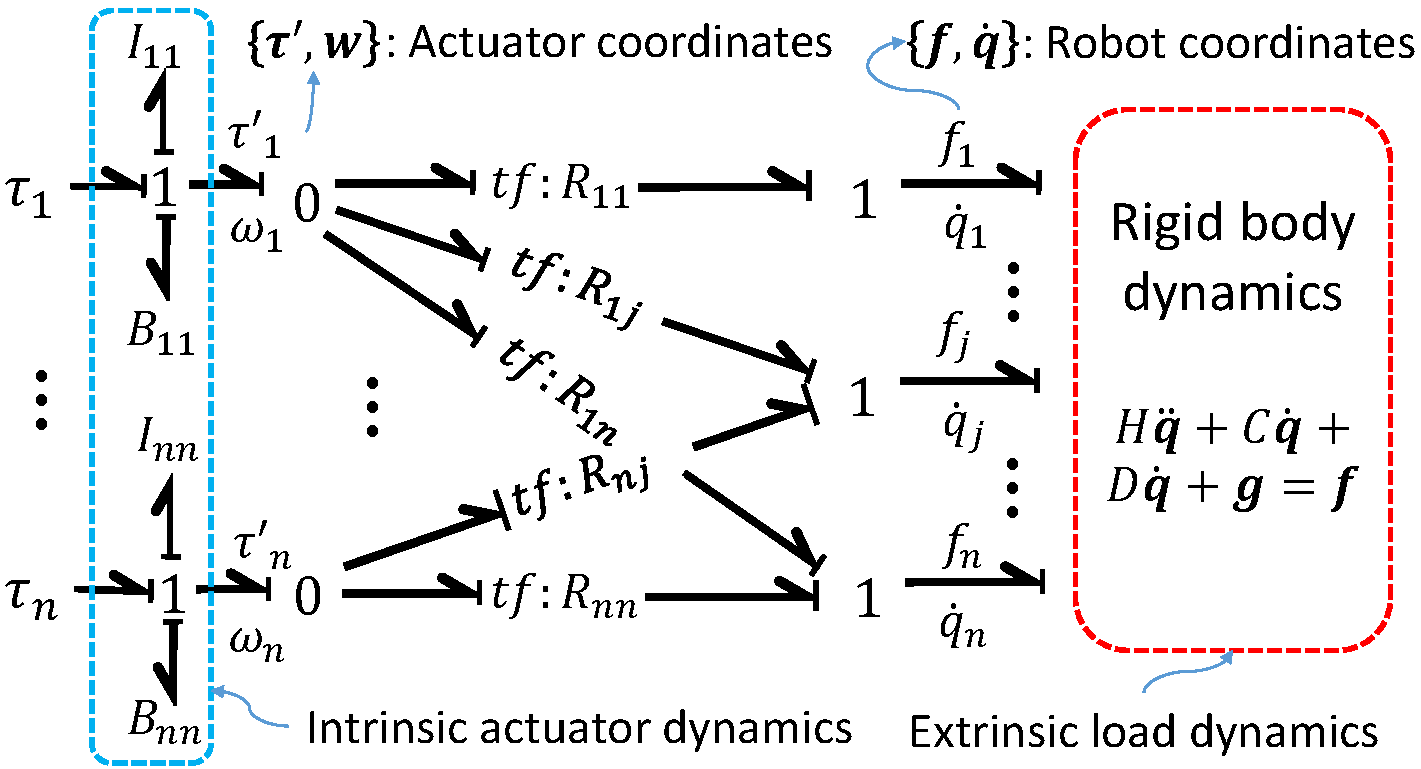
\includegraphics[width=0.70\textwidth]{bondgraph.pdf}
	%\vspace{-10pt}
	\caption{Model of a $n$-Dof robot with variable actuator-joint coupling}
	\label{fig:bondgraph}
\end{figure}

The EoM are then given by:
%
\begin{align}
	&\underbrace{ H \vec{ \ddot{q} } + C\vec{ \dot{q} } + D \vec{ \dot{q} } + \vec{ g } }_{ \vec{\tau}_{E}(\ddot{\vec{q}},\dot{\vec{q}},\vec{q})}
		= R^T \underbrace{  \left[ 
		\vec{ \tau } - I \vec{ \dot{w} } - B \vec{ w }       
		\right]}_{ \vec{\tau}' } 
 \label{eq:eom_ndof}
\end{align}
%
A very wide range of mechanical systems and robots can be represented with this form. Note that, in the case of locomotion or manipulation where the robot interacts with the environment by physically contacting it, the dynamic model $\vec{\tau}_{E}$ must reflect the contact conditions, either by computing contact forces using constraint equations (see section \ref{sec:constraint_forces}) or by formulating $\vec{\tau}_{E}$ as a hybrid dynamical system.

In most practical cases, each actuator has its independent variable transmission and, thereby, the $R$ matrix will be diagonal and each diagonal value can be selected independently. Assuming this situation, the EoM can be simplified to a form, similar to the scalar case, illustrating the effect of the gear ratios matrix $R$: 
%
\begin{align}
	\vec{\tau} &= R^{-1} 
	\underbrace{ 
	\vec{\tau}_{E}(\ddot{\vec{q}},\dot{\vec{q}},\vec{q}) 
	}_{\text{External load dynamics}}
	+ R 
	\underbrace{ 
	\vec{\tau}_{I}(\ddot{\vec{q}},\dot{\vec{q}})
		}_{\text{Intrinsic losses}}
		\label{eq:eom_ndof2}
	\\ %&\text{where} \;
	\vec{\tau}_{E} &\triangleq H \vec{ \ddot{q} } + C\vec{ \dot{q} } + D \vec{ \dot{q} } + \vec{ g } \\
	\vec{\tau}_{I} &\triangleq I \vec{ \ddot{q} } + B \vec{ \dot{q} } 
	%[ \vec{\tau}_{I} ]_j &\triangleq [I]_{jj} [\vec{ \ddot{q} }]_j + [B]_{jj}  [ \vec{ \dot{q} }]_j  \quad \forall j \in {1,2,...,n}
\end{align}
%
The derivation of this simplified form is available in the Appendix \ref{sec:Rdiagndof}.

\subsection{Limitation of the simplified model}
\label{sec:limitation}
%
The main assumption of the proposed model is that gear-ratios are considered as independent control inputs, neglecting all the dynamics and delays associated with changing the gear-ratios. For a system with discrete gear-ratio, transient behaviors from one gear-ratio to another are thus neglected. Physically this implies that the kinetic energy of the system may be discontinuous at a gear-shift since the energy necessary for the transition is not considered. In the case of a car transmission for instance, this model would not keep track of the energy used for accelerating or braking the engine during the synchronization process. This model can be used if the gear-shift process is fast compared to the dynamics of the robots and if the energetic losses due to the gear-shift are negligibly small. Note that, for the DSDM-Arm presented in this thesis, this modeling assumption is supported by the characteristic of DSDM actuators, which can change gear-ratios quickly and seamlessly. For a robot equipped with continuously varying transmissions (CVT), this model would neglect forces associated with the rate of change of the gear-ratios $\dot{R}$, a type of quasi-steady assumption. 
%
In addition, this model also assumes that all motor rotors are in an inertial reference frame, neglecting gyroscopic effects, which may be induced when the axes of motor rotors are rotated.

\subsection{Uncertainty}
\label{sec:uncertainty}

Here, two observations are made regarding the effect of the gear-ratios on disturbances. First, considering modeling errors and external forces on the extrinsic side as unknown generalized forces $\vec{d}$, the EoM given by eq. \eqref{eq:eom_ndof2} becomes:
\begin{align}
	\vec{\tau} &= R^{-1} 
	\vec{\tau}_{E}(\ddot{\vec{q}},\dot{\vec{q}},\vec{q}) 
	+ R 
	\vec{\tau}_{I}(\ddot{\vec{q}},\dot{\vec{q}})
    + R^{-1}
    \underbrace{ 
	\vec{d}
	}_{\text{Disturbances}}    
 \label{eq:eom_ndof3}
\end{align}
where it is assumed that the actuators are accurately modeled. Note that the effect of the disturbances is inversely proportional to the gear-ratios, and thereby attenuated when using large gear-ratios. 

Second, large gear-ratios also decrease the sensitivity of the system to uncertainty. The error on accelerations computed with the inverse dynamic model, will be attenuated with large gear-ratios because of the larger actuator inertia reflected to the extrinsic side:
\begin{align}
	\vec{\ddot{q}}_e &= \vec{\ddot{q}} - \vec{\ddot{q}}_r = 
	\left[ 
    H + R^T I_a R
	\right]^{-1}
    \vec{d}
 \label{eq:sens}
\end{align}
%
Hence, selecting large gear-ratios makes the system less sensitive to uncertainty on the extrinsic side.

\subsection{Hybridness with discrete gear-ratios}
\label{sec:hyb}

When the variable transmissions have discrete configurations, the gear-ratios matrix can only take a set of discrete value:
%
\begin{align}
	R_k \in \{R_1,R_2, ... , R_l\} 
\end{align}
%
where the variable $k$ is a label indexing the different hybrid operating modes of the system, and $l$ is the total number of discrete operating modes. The subscript $k$ will be used to specify a variable specific to a discrete gear-ratios mode. The inverse dynamics equation takes the form:
%
\begin{align}
	\vec{\tau}_k =  R_k^{-1} \vec{\tau}_E + R_k \vec{\tau}_I + R_k^{-1} \vec{d} \quad\forall \; k
\end{align}
%
Where $\vec{\tau}_k$ represent the torque $\vec{\tau}$ when using gear-ratios $R_k$. Note that the defined sum of extrinsic forces $\vec{\tau}_I$ and extrinsic forces $\vec{\tau}_E$, are not function of gear-ratios and are thus the same for every discrete mode $k$. 

The equations of motions thus now have a hybrid nature. With the assumption that transitions are seamless however, states are continuous when gear-ratios changes, and the system is called a switched system \cite{liberzon_switching_2003}. The differential equations are discontinuous, but there is no instantaneous jumps in states. The forward dynamics equation takes the following form:
%
\begin{align}
	\ddot{q}  &=  H_k^{-1} \left[ R_k \tau - \vec{c}_k( \dot{\vec{q}} , \vec{q} ) + \vec{d} \right] \quad\forall \; k 
\end{align}
%
where 
%
\begin{align}
	H_k       &=  H + R_k^T I R_k \\
	\vec{c}_k &=  \left[ C(\dot{\vec{q}} , \vec{q}) + D + R_k^T B R_k  \right] \dot{\vec{q}} + \vec{g}( \vec{q} ) 
\end{align}
%
Note that here the discrete mode $k$ is considered a control input, since it represent the gear-ratios selection.

%%%%%%%%%%%%%%%%%%%%%%%%%%%%%%%%%%%%%%%%%%%%%%%%%%%%%%%%%%%%%%%%%%%%%%%%%%%%%%%%%%%%%%%%%%%%%%%%%%%%%%%%%%%%%%%%%%

\newpage

\section{Optimal gear-ratios along a trajectory}
\label{sec:optigeartraj}

This section analyzes the optimal gear-ratios at each instant along a known trajectory. By looking backward at the situation,  i.e. by evaluating necessary torques and other properties dependent on gear-ratios on a given trajectory, the situation is simplified. For any point on a given trajectory, accelerations $\ddot{\vec{q}}$, speeds $\dot{\vec{q}}$ and positions $\vec{q}$ are known, and then necessary torques $\vec{\tau}$ are only a function of the gear-ratios, which are the only remaining free parameters.

\subsection{Selection criteria}
\label{sec:GearSelectionCriteria}

The two main advantages of changing gear-ratios are 1) lowering the necessary torque to follow a trajectory, 2) modifying the effective impedance reflected on the environment and 3) avoiding rotor-speed limits. 

\paragraph{Torque}
Optimization for reducing torque can be done by minimizing $\vec{\tau}^T \vec{\tau}$ at each point along the trajectory, over all possible gear-ratios. More generally a quadratic function $\vec{\tau}^T Q \vec{\tau}$ could be used to weight each actuator differently.

\paragraph{Impedance}
Optimization for reflected impedance can be done by minimizing the difference between desired task-space impedance and the actual one, which is directly affected by the matrix $R$. The end-point inertia matrix contains the gear ratios: 
%
\begin{align}
	M = [J(\vec{q})^T]^{-1} \big [ H( \vec{q} )  + \underbrace{ R^T I R }_{\text{Actuator contribution}}  \big ] J(\vec{q})^{-1}
 \label{eq:endpointmass}
\end{align}
%
The natural viscous damping reflected to the end-point is also influenced by gear-ratios:
\begin{align}
	V = [J(\vec{q})^T]^{-1} \big [ D + \underbrace{ R^T B R }_{\text{Actuator contribution}}  \big ] J(\vec{q})^{-1}
 \label{eq:endpointdamp}
\end{align}

\paragraph{Constraints}
Another point of practical importance is that $R$ should be constrained to values not leading to rotor velocities $\vec{w}=R \dot{\vec{q}}$ exceeding their maximum speed. This is to avoid solutions with infeasible gear shifts, for example using the low gear at a high speed is impossible. Motor torque saturation could also be included by adding domain constraints on motor torques.

\subsection{Optimization Formulation}
The optimal gear-ratios are determined by minimizing the total actuator torques and, optionally, the difference in end-point impedance:
%
\begin{align}
	R^{*}(\ddot{\vec{q}},\dot{\vec{q}},\vec{q}) &= \operatornamewithlimits{argmin}\limits_{R} \left[ \vec{\tau}^T \vec{\tau} + \alpha_1 \| M_{d} - M \| + \alpha_2 \| V_{d} - V \| \right]  \\
	& \text{s.t}  \quad R \dot{\vec{q}} \leq \vec{w}_{max} 
\label{eq:rmin_general}
\end{align}
%
where $\alpha_i$ are parameters to set the trade-off between minimizing motor torques and matching the desired impedance. Note that torques $\vec{\tau}$ can be substituted by the EoM in the inverse dynamic form (eq. \eqref{eq:eom_ndof2}), and the minimized cost is a function of gear-ratios $R$, accelerations $\ddot{\vec{q}}$, speeds $\dot{\vec{q}}$ and positions $\vec{q}$. 
%

\subsection{Minimal Torque Solution}

For a 1-DoF system, the optimal gear ratio leading to minimal torque, not considering any constraints, at a given instant on a trajectory is given by
%
\begin{align}
	R^{*} &= \operatornamewithlimits{argmin}\limits_{R} \left[ \tau^2 \right] = \sqrt{ \left | \frac{\tau_{E}(\ddot{q},\dot{q},q)}{\tau_{I}(\ddot{q},\dot{q})} \right |   } 
\label{eq:aaa}
\end{align}
%
The derivation is available in the Appendix \ref{sec:optgearproof1}.

Similarly for a multi-DoF system, if $R$ is a diagonal matrix, the optimal gear-ratios can be obtained independently for each axis:
%
\begin{align}
	%R^{*} = \operatornamewithlimits{argmin}\limits_{R} \left[  \vec{\tau}^T \vec{\tau} \right] \Rightarrow 
	[R^*]_{ii} = \sqrt{ \left | \frac{ [\vec{\tau}_{E}(\ddot{\vec{q}},\dot{\vec{q}},\vec{q})]_i }{ [\vec{\tau}_{I}(\ddot{\vec{q}},\dot{\vec{q}})]_i } \right | }
 \label{eq:rmin2}
\end{align}
%
The derivation is available in the Appendix \ref{sec:optgearproofn}.

Note that large gravitational forces or external disturbances, only present in $\vec{\tau}_{E}$, will usually lead to larger optimal gear-ratios, unless they cancel-out other forces in a way that makes $\vec{\tau}_{E}$ smaller. If inertial or viscous forces, present both in $\vec{\tau}_{E}$ and $\vec{\tau}_{I}$, dominate, then the optimal gear-ratios will be a compromise such that extrinsic and intrinsic forces are balanced, a form of impedance matching. The optimal gear ratio given by \eqref{eq:rmin2} includes both gravity, inertial and viscous effects as well as all other effects, hence it can be applied to any arbitrary dynamic situations.


\subsection{Reduction to impedance matching}
\label{sec:impreduc}

In simplified situation where there is only one type of force acting on the system, the general solution reduce to a case of impedance matching. For instance if only inertial forces are involves:
%
\begin{align}
	R^{*}  = \sqrt{ \left | \frac{H \ddot{q} }{ I \ddot{q} } \right |   } = \sqrt{ \frac{H}{I}}  \quad\Rightarrow\quad  {R^{*}}^2 I = H
 \label{eq:impmatchingHI}
\end{align}
%
Hence the optimal gear-ratio is the one for which the external load inertia is equal to the reflected actuator inertia. Also, if only linear dissipative forces are involves:
%
\begin{align}
	R^{*}  = \sqrt{ \left | \frac{D \dot{q} }{ B \dot{q} } \right |   } = \sqrt{ \frac{D}{B}}  \quad\Rightarrow\quad  {R^{*}}^2 B = D
 \label{eq:impmatchingDB}
\end{align}
%
Then the optimal gear-ratio is the one for which the external damping coefficient is equal to the effective actuator damping coefficient reflected to the output. Note that those optimal solutions are only valid locally. In general for robotic systems, $H$ and $D$ are state dependent. 


\newpage

\subsection{Examples of optimal gear-ratios in simple scenarios}
\label{sec:Examples}

Here eq. \eqref{eq:aaa} is applied to the robot in Fig. \ref{fig:bigpicture}, an inverse pendulum with an actuators equipped with a CVT, in simple scenarios. 

\paragraph{Acceleration from rest} 

When the robot accelerates from rest with no viscous forces, the optimal gear ratio at the up-right position, where no gravity acts, is given by:
\begin{align}
	R^{*}  = \sqrt{ \left | \frac{H \ddot{q} }{ I \ddot{q} } \right |   } = \sqrt{ \frac{H}{I}}
 \label{eq:impmatchinginertia}
\end{align}
In this situation, the problem is reduced to impedance matching for two inertial loads. The optimal gear ratio minimizing the torque for a given acceleration is the one for which the load inertia and the motor reflected inertia are the same.

\paragraph{Supporting gravity without moving}

In the situation where the robot is not moving and fighting against gravity, then the optimal gear ratio is:
\begin{align}
	R^{*}  = \sqrt{ \left | \frac{ \vec{g} }{ 0 } \right |   } \rightarrow \infty
 \label{eq:gravrejection}
\end{align}
In this static case, the largest possible gear-ratio is the optimal choice. 


\paragraph{Coasting} 

In the situation where a robot maintains a constant speed, assuming the output load is purely inertial and not dissipative ($D=0$), but that there is friction in the motors:
%
\begin{align}
	R^{*}  = \sqrt{ \left | \frac{D \dot{q} }{ B \dot{q} } \right |   } = \sqrt{ \frac{D}{B}} \rightarrow 0
 \label{eq:coastingex}
\end{align}
%
In this situation, to avoid dissipative motor forces it is best to have the smallest possible gear-ratio. In the limit, this corresponds to completely disconnecting the load from the actuator.

%\paragraph{Resisting disturbances}
%%
%In the situation where there is no gravity and the robot is not moving, but disturbances are expected, minimizing the sliding mode torque (eq. \eqref{eq:rstar_sliding}) would also lead to the conclusion that the largest possible gear-ratio is the optimal choice.
%\begin{align}
	%R^{*}  = \sqrt{ \left | \frac{ 0 + | d |_{max} \, sgn( s ) }{ 0 } \right |   }  = \sqrt{  \frac{| d |_{max} }{ 0 } }\rightarrow \infty
 %\label{eq:gravrejection}
%\end{align}


%%%%%%%%%%%%%%%%%%%%%%%%%%%%%%%%%%%%%%%%%%%%%%%%%%%%%%%%%%%%%%%%%%%%%%%%%%%%%%%%%%%%%%%%%%%%%%%%%%%%%%%%%%%%%%%%%%%%


\newpage

\section{Model-based Controllers}
\label{sec:HierachicalControlApproach}


\begin{flushright}
\textit{"If you know the enemy and know yourself, you need \\ not fear the result of a hundred battles."}  \emph{-- Sun Tzu}
\end{flushright}
\vspace{+10pt}


In this section, control algorithms relying on a dynamic model of a robot and its load are proposed. Methodologies are proposed to synthesize feedback laws, for both the torques and gear-ratios input variables, to follow a trajectory with minimal effort. 


\subsection{R* Computed Torque}
\label{sec:RobustTrajectoryFollowingController}


The proposed closed-loop controller, shown in Fig. \ref{fig:Rstar_block_big}, is based on the Computed Torque technique (see any robotic textbook such as \cite{asada_robot_1986}), but includes an optimization step to compute and select the optimal gear-ratios. As explored in section \ref{sec:dsdm_exp}, when accelerations, speeds and positions are given, locally optimal gear-ratios can be computed. The idea is thus as follow, first compute a desired instantaneous acceleration $\ddot{\vec{q}}_r$ leading to guaranteed convergence to the desired trajectory:
%
\begin{align}
\ddot{\vec{q}}_r &= \ddot{\vec{q}}_d + K_D ( \dot{\vec{q}}_d - \dot{\vec{q}} ) + K_P ( \vec{q}_d - \vec{q} ) 
\end{align} 
%
Then given the actual position $\vec{q}$, actual speed $\dot{\vec{q}}$ and desired instantaneous acceleration $\ddot{\vec{q}}_r$, extrinsic and intrinsic forces for this dynamic state are computed:
%
\begin{align}
	&\vec{\tau}_{E} = H \vec{ \ddot{q}_r } + C\vec{ \dot{q} } + D \vec{ \dot{q} } + \vec{ g } \quad
	&\vec{\tau}_{I} = I \vec{ \ddot{q}_r } + B \vec{ \dot{q} } 
\end{align}
%
Then the controller computes and executes the locally optimal gear-ratios $R^*$, as described previously for a known trajectory, and execute the corresponding motor torques: 
%
\begin{align}
R^{*} &= \operatornamewithlimits{argmin}\limits_{R} \left[ \vec{\tau}^T\vec{\tau}  \right] \quad\text{where}\quad \vec{\tau} = R^{-1} \vec{\tau}_{E} + R \vec{\tau}_{I}
\\
\vec{\tau}^* &= (R^*)^{-1} \vec{\tau}_{E} + R^* \vec{\tau}_{I}
\end{align} 
%
Note that here a simple minimum torque square objective is illustrated for simplicity, but more complex cost functions can be used. As discussed in sec. \ref{sec:optigeartraj}, more complex objectives for optimizing gear-ratios are possible, for instance including motor constraints, desired impedance, etc. 


The salient feature of the R* Computed Torque controller is that the optimal gear-ratios is selected based on state-feedback, i.e. even in situations not foreseen in the planner that generated the nominal trajectory. For instance, if a disturbance pushes the robot in a state where the robot faces a large gravitational force requiring a large gear-ratio, the controller will automatically select it. Similarly if facing a contact force, that is included in the model, the R* controller will automatically select the appropriate gear-ratio. Fig. \ref{fig:dq} offer a graphical interpretation of the R* algorithm in the phase plane. 

\begin{figure}[t]
	\centering
		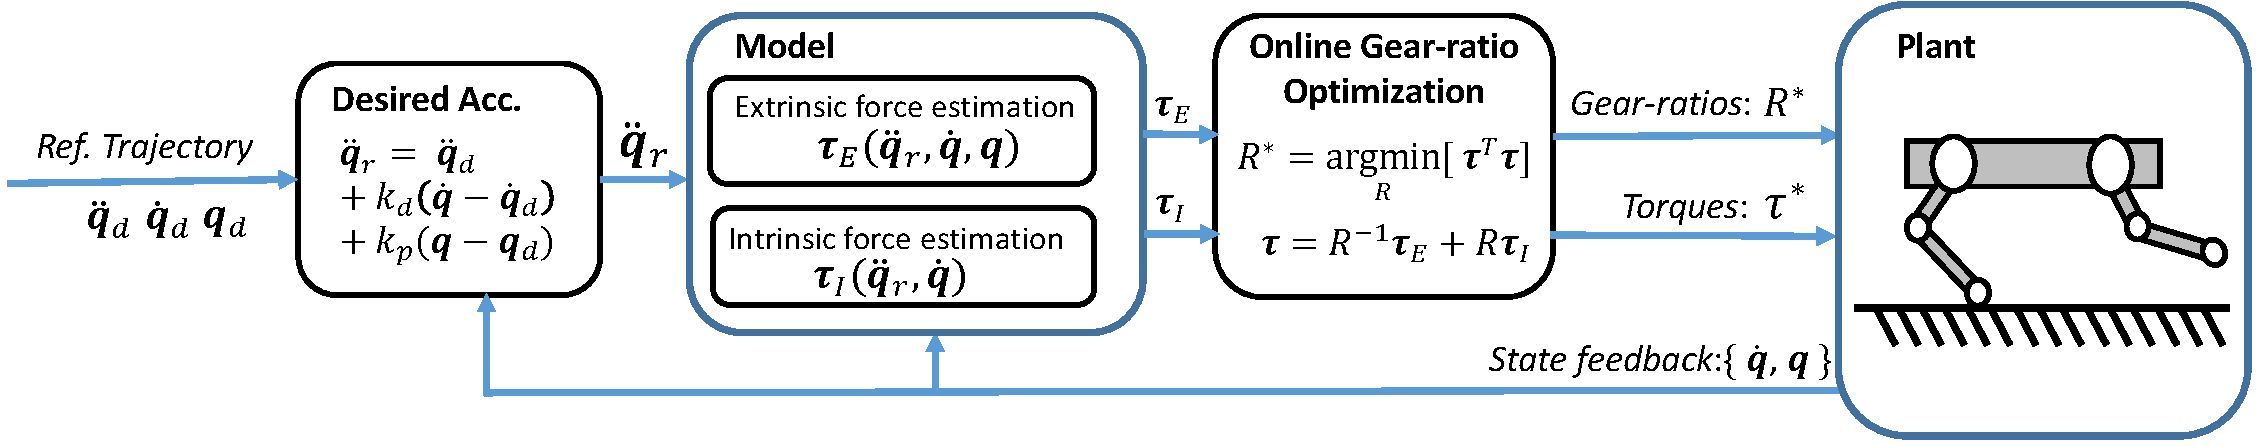
\includegraphics[width=0.99\textwidth]{Rstar_block_big.pdf}
	\caption{R* Computed Torque controller}
	\label{fig:Rstar_block_big}
\end{figure}

\begin{figure}[htp]
	\centering
		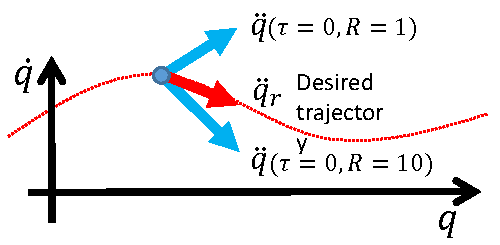
\includegraphics[width=0.50\textwidth]{dq.pdf}
	\caption[R* algorithm graphical interpretation]{The R* algorithm can be interpreted graphically, as selecting the gear-ratios for which the natural acceleration vector is the closet to the desired instantaneous acceleration vector $\vec{\ddot{q}}_r$ (after scaling the distance with the inertia), in order to minimize the necessary torques to apply on the system.}
	\label{fig:dq}
\end{figure}

\subsection{R* Sliding Mode Control}
\label{sec:slidingmode}

In general Computed Torque Control is susceptible to modeling uncertainties and disturbances. This section presents an approach based on sliding mode control \cite{slotine_applied_1991}, to improve robustness and guaranteeing performance despite uncertainty. Moreover, the presented control algorithm leverages the gear-ratios options to decrease sensitivity of the robot to disturbance when uncertainty is large. The control scheme is illustrated at Fig. \ref{fig:sliding_blocks}.

First, the following intermediary variables are computed:
%
\begin{align}
	&\vec{q}_e        = \vec{q}          -  \vec{q}_d   \quad\quad
	&\dot{\vec{q}}_e  = \dot{\vec{q}}    -  \dot{\vec{q}}_d \\
	&\vec{s}          = \dot{\vec{q}}_e  +  \lambda \vec{q}_e \quad\quad
  &\vec{\ddot{q}}_r = \ddot{\vec{q}}_d -  \dot{\vec{q}}_e 
 \label{eq:slidingvar}
\end{align}
%
As for the R* Computed Torque, intrinsic and extrinsic forces are then computed for this dynamic state:
%
\begin{align}
	&\vec{\tau}_{E} = H \vec{ \ddot{q}_r } + C\vec{ \dot{q} } + D \vec{ \dot{q} } + \vec{ g } \quad
	&\vec{\tau}_{I} = I \vec{ \ddot{q}_r } + B \vec{ \dot{q} } 
\end{align}
%
The instead of simply using the inverse dynamic equation to compute torques, a discontinuous gain is added:
%
\begin{align}
	\vec{\tau} &=  R^{-1} 
	\vec{\tau}_{E}(\ddot{\vec{q}}_r,\dot{\vec{q}},\vec{q}) 
	+ R 
	\vec{\tau}_{I}(\ddot{\vec{q}}_r,\dot{\vec{q}})
  - R^{-1} G sgn( \vec{s} ) 
 \label{eq:slidingctl}
\end{align}
%
Then the controller computes and executes the locally optimal gear-ratios $R^*$, minimizing the sliding mode torque that depends on selected gear-ratios, and execute the corresponding motor torques: 
%
\begin{align}
R^{*} &= \operatornamewithlimits{argmin}\limits_{R} \left[ \vec{\tau}^T\vec{\tau}  \right] \quad\text{where}\quad \vec{\tau} = R^{-1} \vec{\tau}_{E} + R \vec{\tau}_{I} - R^{-1} G sgn( \vec{s} ) 
\\
\vec{\tau}^* &= (R^*)^{-1} \vec{\tau}_{E} + R^* \vec{\tau}_{I} - (R^*)^{-1} G sgn( \vec{s} ) 
\end{align} 
%
\begin{figure}[t]
	\centering
		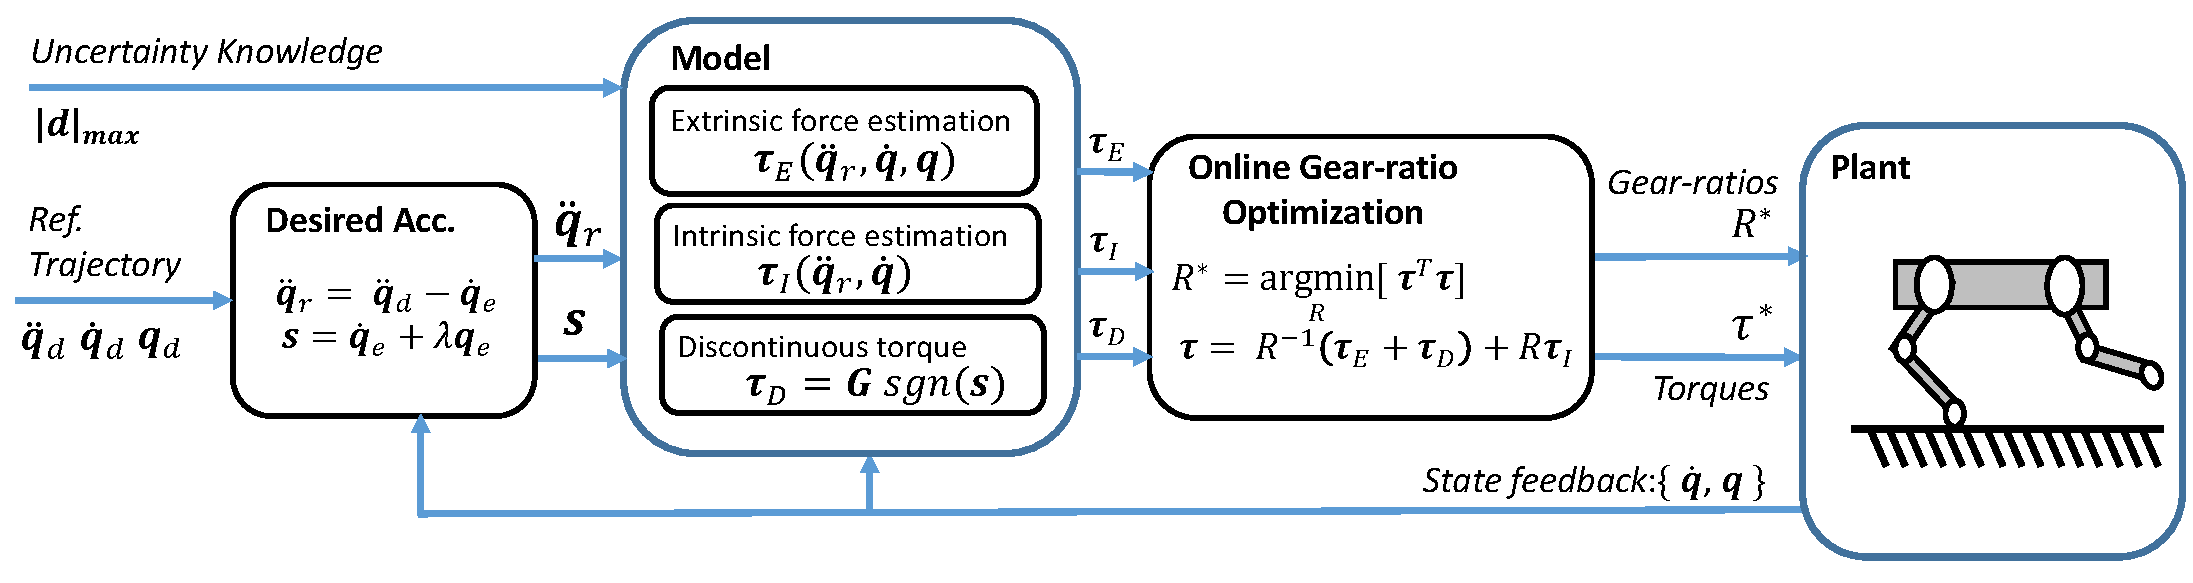
\includegraphics[width=0.99\textwidth]{sliding_blocks.pdf}
	\caption{R* Sliding Mode controller}
	\label{fig:sliding_blocks}
\end{figure}
%
To guarantee convergence despite uncertainty, the discontinuous gain are set as a function of the bounds on uncertainty:
%
\begin{align}
	G &= \left[ H + R^T I R \right] K \\ K_{ii} &> \operatornamewithlimits{max}\limits_{\vec{d}} \left| \left(  \left[ H + R^T I R \right]^{-1} \vec{d} \right)_{i} \right| + \eta
\end{align}
%
where $\vec{d}$ is an unknown generalized force vector, representing modeling uncertainty in the extrinsic dynamics and external disturbances, see section \ref{sec:uncertainty}. Note that the discontinuous gain is a function of the state-dependent inertia matrix, bounds on disturbances and the selected gear-ratios. The interesting features of the R* Sliding Mode Controller is that with gear-ratios selected to minimize the sliding mode torque, then naturally, larger gear-ratios are selected in response to large uncertainty. 

\subsubsection{1-DoF system exemplified} 

To clarify the behavior of R* Sliding Mode, the simplified control laws for a 1-DoF system are analyzed. The feedback law for torque in 1-DoF is reduced to 
%
\begin{align}
	\tau &=  \frac{\tau_{E}(\ddot{q}_r,\dot{q},q)}{R} 
	+ R \tau_{I}(\ddot{q}_r,\dot{q})
  - \frac{G sgn( s ) }{R} 
\end{align}
%
and the discontinuous gain reduced to 
%
\begin{align}
K &= \frac{d_{max}}{H + R^T I R} + \eta \\
G &= \left[ H + R^T I R \right] K  =  d_{max} + \left[ H + R^T I R \right] \eta 
\end{align}
%
Rearranging the torque law gives:
%
\begin{align}
	\tau &=  \frac{\tau_{E}( \overbrace{ \ddot{q}_r - \eta sgn( s ) }^{\ddot{q}_a},\dot{q},q) - d_{max} sgn( s )  }{R} 
	+ R \tau_{I}(\overbrace{\ddot{q}_r - \eta sgn( s )}^{\ddot{q}_a} ,\dot{q})
\end{align}
%
Minimizing the torque computed with this sliding mode control law over possible $R$ values, also have an enlightening analytical solution:
%
\begin{align}
	R^{*} &= \operatornamewithlimits{argmin}\limits_{R} \left[ \tau^2 \right] = \sqrt{ \left | \frac{\tau_{E}(\ddot{q}_a,\dot{q},q) + | d |_{max} \, sgn( s ) }{\tau_{I}(\ddot{q}_a,\dot{q})} \right |   } 
\label{eq:rstar_sliding}
\end{align}

If no disturbance is expected ($| d |_{max}=0$) then the solution is, as before, a compromise between extrinsic and intrinsic forces. However, knowledge of uncertainty in the form of disturbances bound modifies the optimal gear-ratios solution. When large disturbances are expected ($| d |_{max}$ is large) the solution is biased toward larger gear-ratios, which is consistent with the sensitivity analysis that concluded that larger gear-ratios attenuate the effect of disturbances. All in all, minimizing torque computed with the sliding mode law, is a way to naturally improve the decision regarding the best gear-ratios, in function of some knowledge of the expected uncertainty.
%

\subsection{Adaptation}
If the uncertainty is structured as unknown model parameters in the extrinsic dynamics, the term represented by $\vec{\tau}_E$, then traditional adaptation schemes can be used for estimating the unknown parameters. Then, if adaptation converges to the correct computed torque, then the computed best gear-ratios will also converge to the true optimal gear-ratios:
%
\begin{align}
	\hat{\vec{\tau}}_E \rightarrow \vec{\tau}_E 
    \quad \Rightarrow \quad 
    \hat{R}^* \rightarrow R^*
 \label{eq:adapt}
\end{align}
%
If used in conjunction with the R* Computed Torque controller, decisions regarding the optimal gear-ratios would improve as adaptation converges. Note that correct gear-ratios decision depends on the correct estimation of extrinsic torque, not model parameters explicitly, which are harder to estimate since requiring condition related to sufficient excitation. 

As an example, for a 1-DoF robot with the following EoM:
%
\begin{align}
	\left[ H + R^2 I \right] \ddot{q} + \left[ R^2 B \right] \dot{q} + \left[ mg \sin( q ) \right] = R \tau
\end{align}
%
the regression to identify unknown extrinsic parameters $H$ and $m$, could be built this way:
%
%
\begin{align}
	\overbrace{
	\underbrace{ \left[
	\begin{array}{c c}
		\frac{\ddot{q}}{R} &  \frac{ g \sin( q ) }{R}
	\end{array} \right] }_{\vec{\phi}}
	\underbrace{ \left[
	\begin{array}{c}
		H \\ m 
	\end{array} \right] }_{\vec{\theta}}
	}^{\tau_E} = \underbrace{ \tau -  \overbrace{ R I \ddot{q} -  R B \dot{q} }^{\tau_I} }_{y}
\end{align}
%
where $\vec{\theta}$ is a vector of unknown parameters, $\vec{\phi}$ is a known regressor vector (the controller is always aware of the selected gear-ratio $R$) and $y$ is a known scalar output. 

Adaption on both the extrinsic and intrinsic dynamic parameters could also be conducted, with a regression constructed this way:
%
\begin{align}
	\underbrace{ \left[
	\begin{array}{c c c c}
		\frac{\ddot{q}}{R} &  R\ddot{q} & R \dot{q} & \frac{ g \sin( q ) }{R}
	\end{array} \right] }_{\vec{\phi}}
	\underbrace{ \left[
	\begin{array}{c}
		H \\ I \\ B \\ m
	\end{array} \right] }_{\vec{\theta}}
	 = \underbrace{ \tau }_{y}
\end{align}
%
However, care would need to be used since the first two terms in the regression vector would be fully correlated if data using a single gear-ratio is used, which makes the solution ambiguous in term of possible $H$ and $I$ parameters. If data with multiple different gear-ratios is used, then all terms could be independently identified. 


\subsection{Generalization to more complex models}

Many modeling assumption, for instance leading to extrinsic vs. intrinsic force separation, were assumed to hold during the control algorithm presentations mainly because it gives many physical insight. However, this restricted class of model is not necessary to implement the proposed algorithms, the minimum needed is to have a model of the inverse dynamic, which could include any non-linearity, in the form:
%
\begin{align}
	\vec{\tau}  = f( \vec{\ddot{q}}_r , \vec{\dot{q}} , \vec{q} , R )
\end{align}
%
to compute necessary torque $\vec{\tau}$ to achieve a specified acceleration $\vec{\ddot{q}}_r$, given actual states $(\vec{\dot{q}} , \vec{q})$ and selected gear-ratios $R$.

%PFL

\subsection{Closed-loop selection of discrete gear-ratios}

So-far the proposed control schemes made no assumption regarding the different gear-ratios options, and analytical solutions assumed that gear-ratio have continuous domains. However, many variable transmission mechanisms, such as the DSDM actuator technology proposed in this thesis, offer only a discrete set of possible values. In that situation, the optimization step in the proposed control algorithms would then be a combinatorial optimization problem. However, if the number of options $l$ is reasonably small, then every possible options can be computed quickly to find the optimal discrete option:
%
\begin{align}
k^{*} &= \operatornamewithlimits{argmin}\limits_{k} \left[  \vec{\tau}_1^T\vec{\tau}_1  , ... , \vec{\tau}_k^T\vec{\tau}_k , ...  , \vec{\tau}_l^T\vec{\tau}_l \right]
\end{align}
%
In practice this brute force approach is usually feasible. For instance, for the robot presented in this thesis, there is 3 actuators each with 2 gear-ratios options, leading to only $l=2^3=8$ possible matrix $R$.

\subsubsection{Point-by-point}

In theory if the controlled robotic system would behave exactly like the proposed model, then selecting optimal gear-ratios at each time steps would be the optimal behavior. However, because the control effort associated with gear-shifts is neglected in the model and the basic gear-selection scheme does not penalize mode transitions, using the proposed controller can lead to rapid switching between gear-ratios (chattering) in certain situations. In practice, this is not desirable since for most type of variable transmissions, since changing the gear-ratio: 1) is not really instantaneous 2) the shifting process would require some effort/energy 3) fast switching can lead to mechanical wear and also excite un-modeled vibration modes. 

\subsubsection{Hysteresis}

To avoid undesirable rapid switching behaviors, hysteresis can be added to the gear-selection logic. Instead of simply executing the optimal gear-ratios command at each time step, a logical step is added, which only allows mode change if a minimal amount of time $\Delta t$ as elapsed since the last mode change. This thus directly guaranteed a minimal period between gear-shifts. However, this technique is clearly sub-optimal in certain situations. For instance, imagine a system with two modes, on a trajectory where $k=1$ is optimal for all time except for the interval $t\in[1,1.1]$. If a hysteresis of $\Delta t = 1$ is used in the controller, then $k=2$ will be selected for the interval $t\in[1,2]$. Hence, not gear-shifting at all would have been better (sub-optimal during 0.1 sec) compared to shifting with hysteresis (sub-optimal during 0.9 sec), from the whole trajectory point of view. 

\subsubsection{Minimax optimization for sliding mode}
\label{sec:minimax}

When optimizing the torque computed with the sliding mode, chattering can be very severe as components of $sgn( \vec{s} )$ can oscillate rapidly between values of $\pm1$. One approach to alleviate this is to reformulate the optimization to treat variables $sgn( \vec{s} )$ as random disturbances and optimize for the worst-case scenario:
%
\begin{align}
R^{*} &= \operatornamewithlimits{argmin}\limits_{R} \operatornamewithlimits{max}\limits_{sgn(\vec{s})} \left[ \vec{\tau}^T\vec{\tau}  \right] \quad\text{where}\quad \vec{\tau} = R^{-1} \vec{\tau}_{E} + R \vec{\tau}_{I} - R^{-1} G sgn( \vec{s} ) 
\end{align} 
%
The result of this optimization is independent from the position of states with respect to the switching surface $s=0$, and would remove this source of rapid change of optimal gear-ratios solutions. Also, the sliding mode controller could be implemented with smoothing techniques for the discontinuous torque, many techniques exist \cite{slotine_applied_1991} \cite{perruquetti_sliding_2002}. This would also alleviate one source of chattering for the gear-ratios selection.

\subsection{Rollout gear-ratios selection}

A better approach to the problem of avoiding fast gear-shifting, is to associate a one-time cost with transitions and optimize over a time-horizon. This way a trade-off between changing gear-ratios quickly to minimize torques and minimizing the number of gear-shifts can be formalized.
%
\begin{figure}[tp]
	\centering
		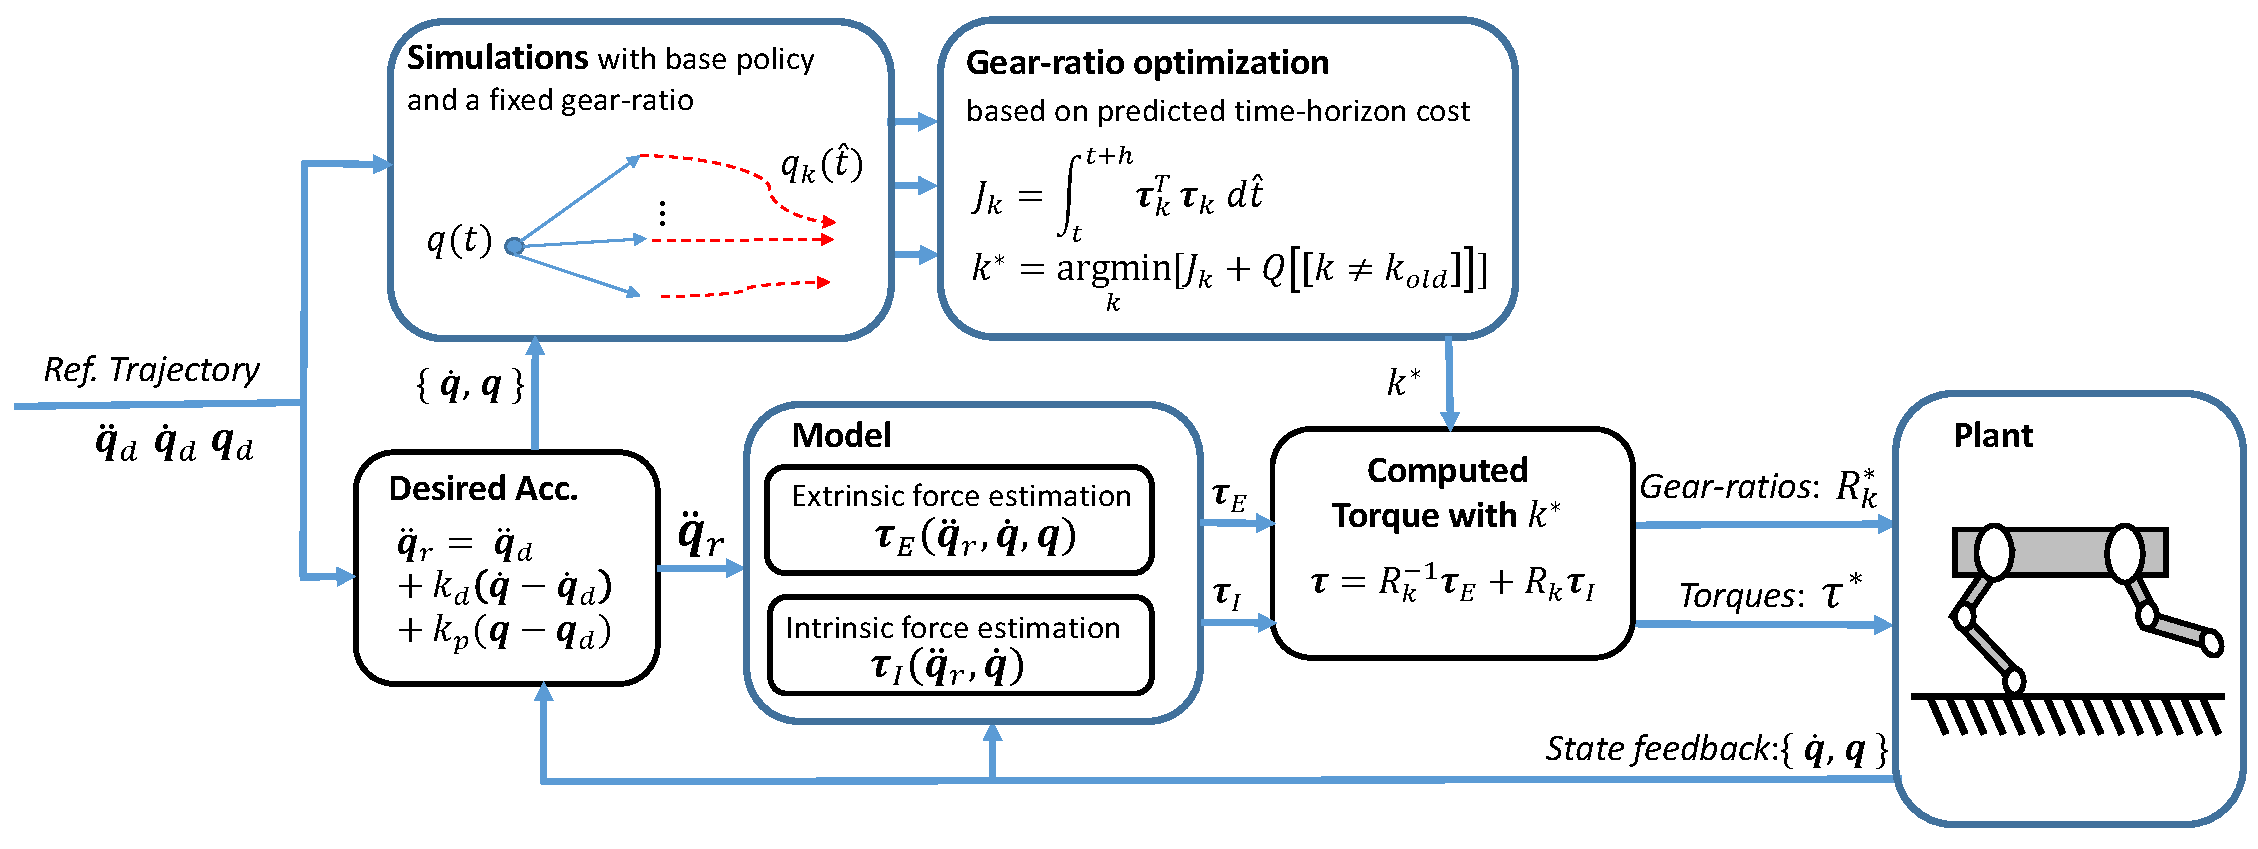
\includegraphics[width=0.99\textwidth]{Rollout_block.pdf}
	\caption{Rollout with Computed Torque Control as base policy}
	\label{fig:Rollout_block}
\end{figure}
%
\begin{figure}[tp]
	\centering
		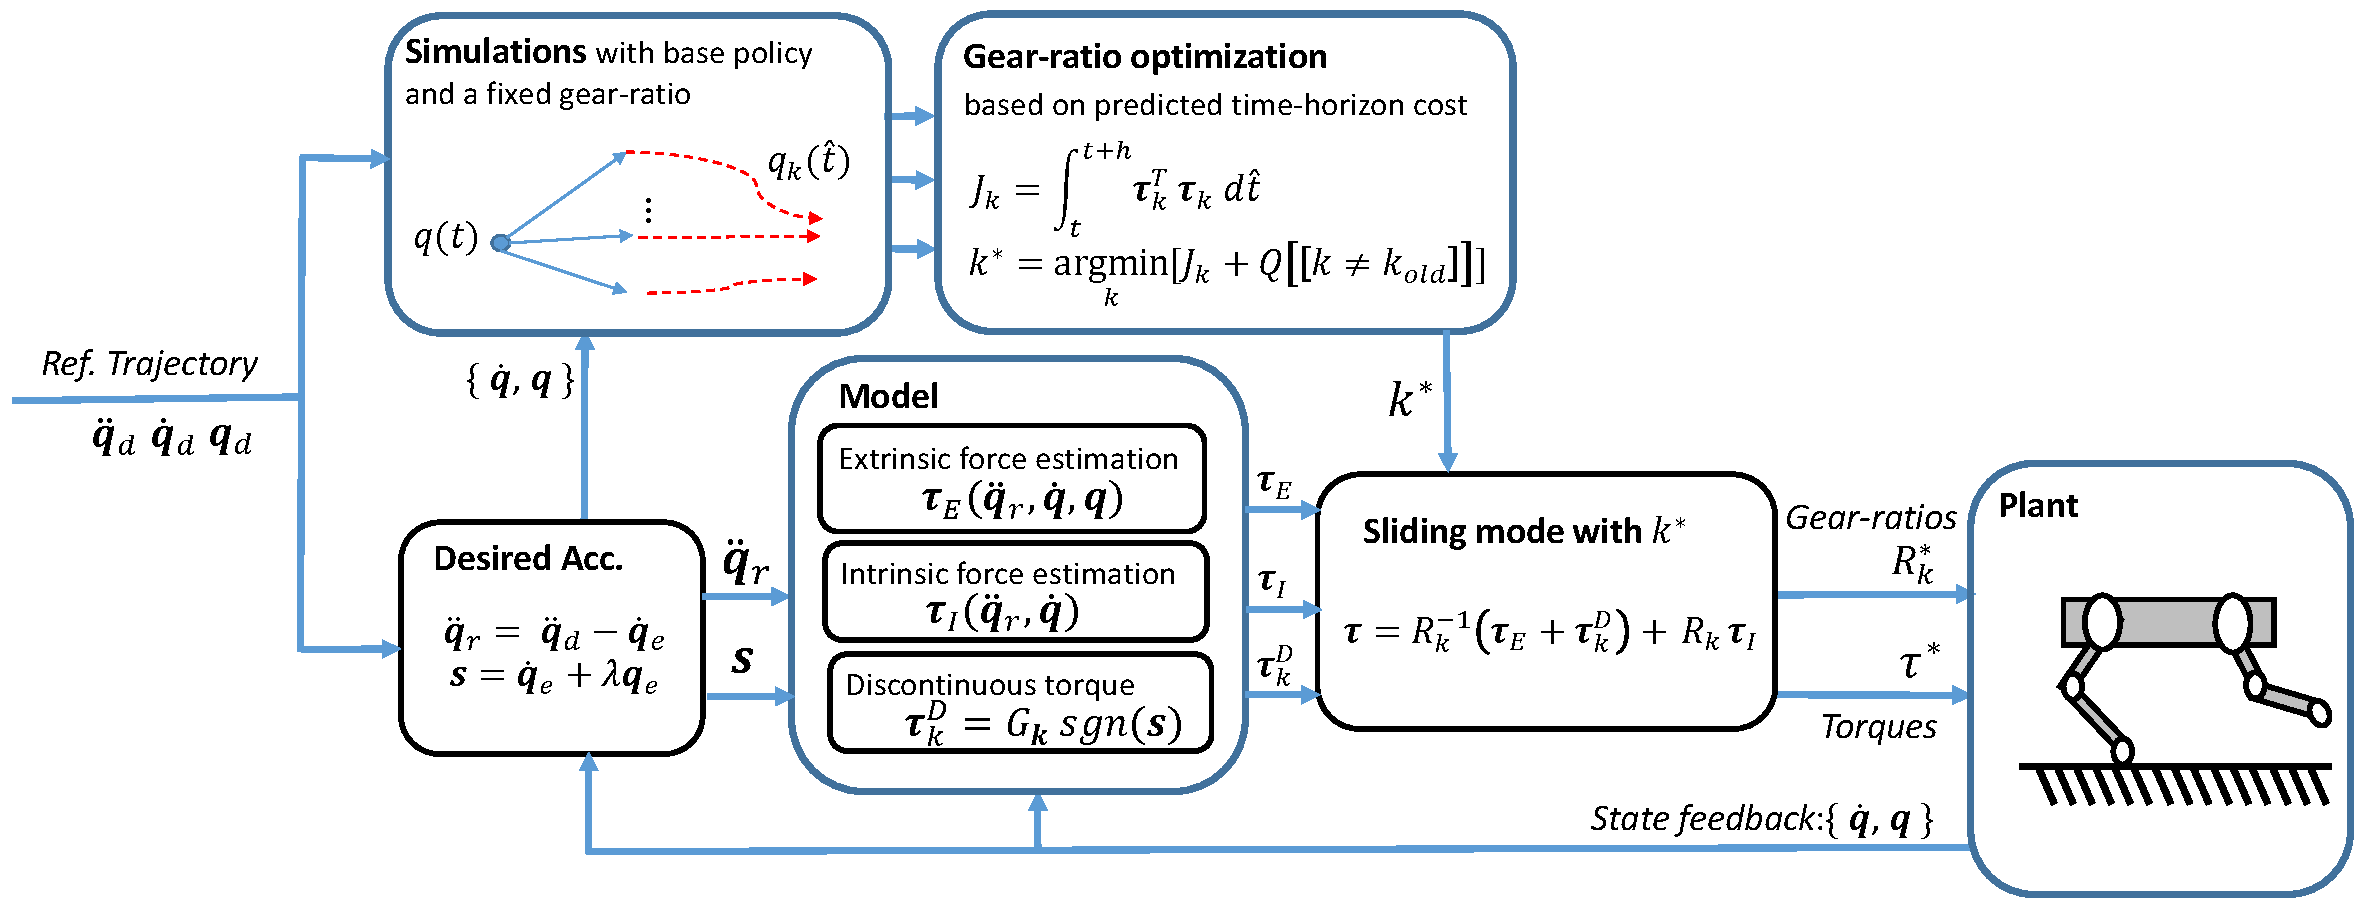
\includegraphics[width=0.99\textwidth]{Rollout_sliding_block.pdf}
	\caption{Rollout with Sliding Mode Control as base policy}
	\label{fig:Rollout_sliding_block}
\end{figure}
%
The proposed approach to implement this idea in a closed-loop control scheme, is to use predictive simulations over a receding time-horizon, analogous to the model predictive control (MPC) approach. Predicted trajectories are computed by simulating the robotic system under the control of a base policy that consist in 1) keep the gear-ratios fixed 2) motor torques controlled with the computed torque or sliding mode feedback law.  The approach is illustrated used in conjunction with a Computed Torque at Fig. \ref{fig:Rollout_block} and sliding mode at Fig. \ref{fig:Rollout_sliding_block}.

An integral cost $J_k$ for each of those $l$ simulated trajectories with fixed gear-ratios is computed:
%
\begin{align}
J_k &= \int_t^{t+h} \vec{\tau}_k^T \vec{\tau}_k d\hat{t}
\end{align}
%
where $t$ is actual real time, $h$ is the horizon, $\hat{t}$ is the simulation time and $\vec{\tau}_k$ are the torques computed with the base policy in the simulations. Once those simulations and integrals are computed, the gear-ratios are selected by conducting the following optimization:
%
\begin{align}
k^{*}      &= \operatornamewithlimits{argmin}\limits_{k} \left[ J_k + Q [[ k \neq k_{last}]] \right] %\\
%\vec{\tau} &= \vec{\tau}_{k^*}( \dot{\vec{q}} , \vec{q} )
\end{align}
%
where $Q$ is the cost penalty for gear-shifting. Hence, optimal gear-ratios, computed at time $t$, are the optimal ones considering an integral cost over the future horizon $h$. Note that state errors are not penalized in the integral cost, because the base policy for motor torques already enforces trajectory tracking. The scheme is illustrated at Fig. \ref{fig:rollout}.
%
\begin{figure}[htp]
	\centering
		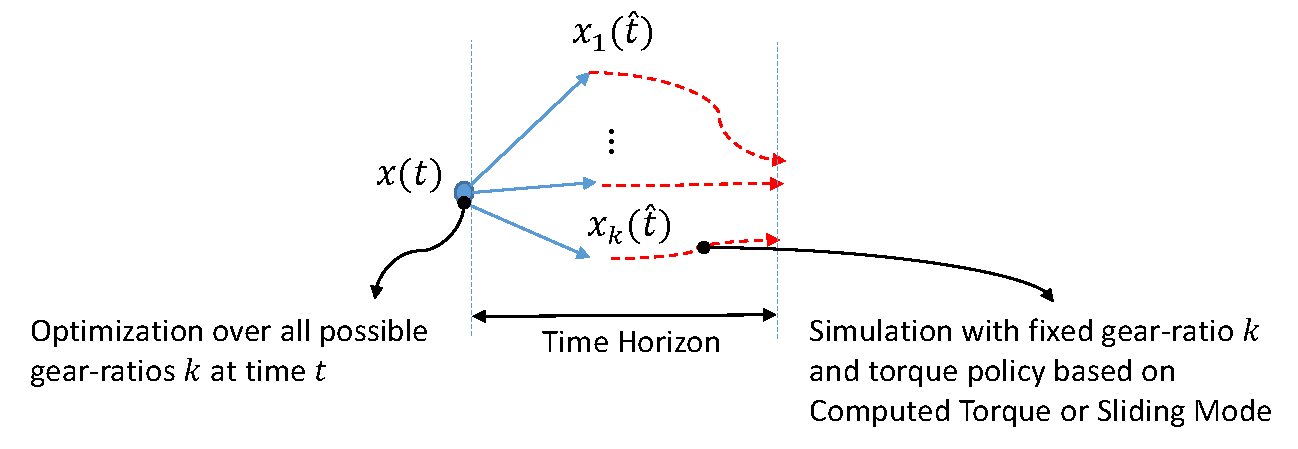
\includegraphics[width=0.85\textwidth]{rollout.pdf}
	\caption[Rollout gear selection]{Rollout gear selection}
	\label{fig:rollout}
\end{figure}


This scheme is closely related to the Rollout control approach \cite{bertsekas_dynamic_2000}, and it will thus be refer to as the Rollout gear-ratios selection.  However here the optimization is conducted only over the gear-ratios options, not all possible control actions at time $t$ like in the original technique. The two reasons for not implementing a full scale optimization including also many possible torque inputs at time $t$ are: 1) computational limitations and 2) by applying the base policy torques at time $t$, convergence to the desired trajectory can be guaranteed. 

Advantageous features of the Rollout gear-selection scheme are 1) filtering-out fast un-desirable gear-shifts 2) commanding gear-shifts in advance, which can compensate for gear-shift delay in the physical system (situation just entering the horizon at time $t+h$ influence the gear-ratios selection at time $t$).

\subsubsection{Extension from Rollout to Model Predictive Control (MPC)}

The proposed control scheme requires simulating $l$ trajectory at each time steps, which is usually tractable computationally. However, this is sub-optimal in the sense that gear-ratios are fixed on each trajectory. With more computational power, additional options of more complex sequences of discrete gear-ratios could be included. Each option of a predetermined sequence of gear-ratios could be seen as a form of motion primitive, a proposed approach to simplify control/planning when the number of possible action is too large to fully explore \cite{gray_predictive_2012}. This would also connect with the idea of family of modes proposed to simplify MPC control of hybrid systems \cite{hogan_feedback_2016}. The proposed Rollout gear-selection scheme, can thus also be seen as optimizing over $l$ motion primitives consisting of using fixed gear-ratios for the next $h$ seconds. 

Furthermore, if the optimization would also be conducted over possible motor torques, instead of constraining them to always follow a given feedback law, then the control scheme would correspond to full scale MPC. However, MPC is in general very hard to implement at satisfactory fast rate for non-linear multi-DOF robotic systems, especially when the system is hybrid \cite{hogan_feedback_2016}. 
%
All in all, depending on the complexity of the controlled robotic system and the available computational power, the proposed control scheme can be adapted from a very easy-to-compute point-by-point optimization with hysteresis, to more optimal but computationally-heavy predictive schemes with a variety of level of complexity. 


\subsection{Stability}

Here stability properties of the proposed control laws are discussed. The main interesting conclusion is that complex gear-selection schemes, such as Rollout, can be implemented in conjunction with the proposed base feedback laws for torques (computed torque or sliding mode), without affecting the stability results. 

\paragraph{R* Computed Torque} Convergence to the desired trajectory, with the R* Computed Torque controller, is guaranteed assuming the model used by the controller is exact. Interestingly this results is valid for any arbitrary sequence of gear-ratios as long as the feedback law computing the continuous torques $\vec{\tau}$ is aware of the discrete operating mode $k$, see details in sec. \ref{sec:stabrstar1}. Hence, any gear-ratios selection scheme can be used, without compromising the convergence to the desired trajectory, including hysteresis, Rollout optimization, etc.

\paragraph{R* Sliding Mode} Guaranteed convergence to the desired trajectory, with the R* Sliding Mode controller, can be extended to situation where the uncertainty can be bounded, assuming gains $G$ are chosen accordingly, see details in sec. \ref{sec:stabrstar2}. Stability is also guaranteed for any sequence of discrete gear-ratios $k$ and thus would not be affected by the closed-loop gear-ratios selection scheme.


\subsection{Chattering and high-frequency switching}

This section discusses results regarding the chattering behavior when using the proposed control schemes. 

\subsubsection{Decision boundaries}

Chattering (quickly selecting back-and-forth) between two discrete mode $i$ and $j$ can occur when the system stay in a dynamic state for which optimized cost is equal for two or more gear-ratios options. For instance with the quadratic torque criterion when:
%
\begin{align}
\vec{\tau}_i^T \vec{\tau}_i = \vec{\tau}_j^T \vec{\tau}_j
\end{align}
%
If the policy for motor torque $\vec{\tau}_k(\vec{x})$ is substituted in the cost equality equation, the result is a decision boundary in the state-space, in the form:
%
\begin{align}
r_{ij} ( \vec{x} ) = 0
\end{align}
%
If $r_{ij}>0$ then the decision is $k=i$, while if $r_{ij}<0$ the decision is $k=j$. When using the R* Computed Torque controller for a 1-DoF system, the decision boundary between $k=i$ and $k=j$ takes the form
%
\begin{align}
0 = r_{ij} ( \vec{x} )  = \left[ \frac{R_i^2-R_j^2}{\frac{1}{R_i^2}-\frac{1}{R_j^2}}\right] - \frac{\tau_E}{\tau_I}
\end{align}
%
Boundary decision could also be created by the inequality constraints in the optimization. The most relevant example is motor speed saturation which can create decision boundaries of the type:
%
\begin{align}
0 = r_{ij} ( \vec{x} )  = w_{max} \pm \frac{\dot{q}}{R_i}
\end{align}
%

\subsubsection{Situations leading to fast gear-ratios switching}

Fig. \ref{fig:chatsit} illustrates different possible class of situations leading to fast switching.
%
\begin{figure}[t]
        \centering
				\subfloat[Staying on the decision boundary]{
        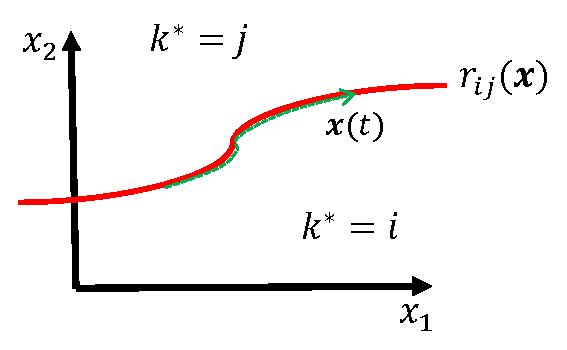
\includegraphics[width=0.30\textwidth]{inv_sur.pdf}
				\label{fig:inv_sur}}
				\hspace{+3pt}
        \subfloat[Decision boundary attracting all trajectory]{
				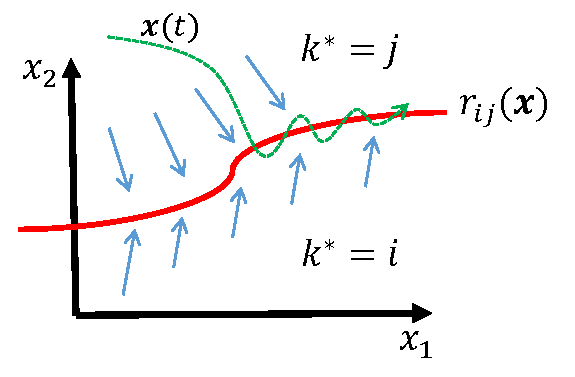
\includegraphics[width=0.30\textwidth]{inv_sld_sur.pdf}
				\label{fig:inv_sld_sur}}
				\hspace{+3pt}
				\subfloat[High-frequency crossing of the decision boundary]{
				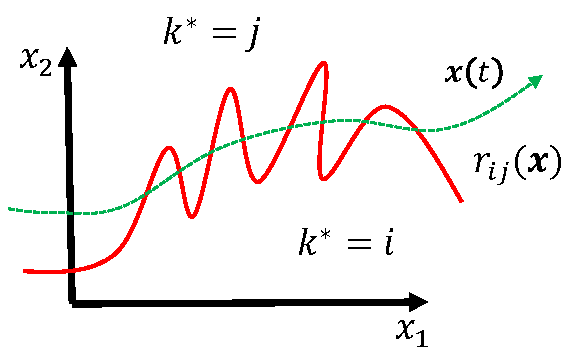
\includegraphics[width=0.30\textwidth]{hifreq_sur.pdf}
				\label{fig:hifreq_sur}}
        \caption[Situations leading to fast gear-ratios switching]{Situations leading to fast gear-ratios switching. $r_{ij}$ is a decision boundary between $k^*=i$ and $k^*=j$ }\label{fig:chatsit}
\end{figure}


The theoretical closed-loop behavior, when exactly on the boundary decision is a degenerative case of ambiguous infinitely fast jumps between gear-ratios. In practical implementations, because decision are delayed, staying in the vicinity of the decision boundary $r_{ij} \approx 0 $ could lead to chattering, with a period depending on implementation aspects such as computing delay, sampling time and hysteresis in the gear-selection logic. 

Fig. \ref{fig:inv_sur} and \ref{fig:inv_sld_sur} illustrate two possible class of behavior for which the system stay in the vicinity of the decision boundary and would lead to chattering behavior. A situation of type (a) represent a case where the system trajectory coincide with the boundary decision and a situation of type (b) represent a more severe case where all trajectory would be attracted to the decision boundary, i.e. a type of undesired sliding mode. Those two types of situation can be ruled-out as impossible, if conditions guaranteeing convergence to the desired trajectory are met. By contradiction, state cannot both converge on the desired trajectory and stay on the decision boundary, unless for very special cases where the desired trajectory is in the sub-domain defined by the decision boundary. 

\paragraph{Example of gear-shift chattering with a car going up-hill}

In practice, a situation of type (b) can be a typical failure mode of switched system. This section explore with a simple example of how this situation can arise and how the proposed control schemes make sure this is avoided. Imagine a car with an automatic transmission going up-hill, with a gear-selection scheme only based on a velocity decision boundary. The car starts from rest with its low-gear $k=1$ and accelerate. After reaching reaching a threshold velocity, the automatic transmission then engage the high-gear $k=2$. With the high-gear however, the effect of gravity is much larger and the car slow down until it cross again the threshold velocity. The low-gear $k=1$ is then engaged again and the car starts accelerating. The car then cross again the threshold and the cycle would continue forever. What is happening here is that the car converge toward its velocity goal when $k=1$ but diverge when $k=2$. With the proposed R* Computed Torque controller, this could happen if gravity forces were underestimated in the model. However, if gravity forces are either correctly modeled, or alternatively included in the uncertainty bounds with the sliding mode controller, then convergence would be guaranteed for both modes, and enough torque to continue accelerating toward the target velocity would have been applied. %Furthermore, if it takes more torque to continuing accelerating with $k=2$, the the R* Computed Torque would not have selected the high-gear in this situation. 

So far, situations of chattering in the vicinity of decision boundary of type (a) and (b), have been ruled-out impossible if the controller is designed to guarantee convergence for all discrete mode $k$. However, situations of type (c), illustrated at Fig. \ref{fig:hifreq_sur} and called high-frequency switching, is still possible and un-desirable. The decision boundary can very complex for highly non-linear systems, hence even a simple trajectory can cross decision boundaries at undesirable high-frequencies. 

\subsubsection{Minimum cycle time with Rollout}

The Rollout approach is efficient to avoid situations of type (c), high-frequency switching. By optimizing over a time horizon, the Rollout gear-selection scheme is acting as a low-pass filter. Moreover, with the Rollout approach, a minimum value for the cycle period of gear-shifting back-and-forth between two gear-ratios can be guaranteed. 

The cycle time $\Delta t$ of gear-shifting from arbitrary mode $i$, to another arbitrary mode $j$, and back to the initial mode $i$, is lower bounded. If the system follows the desired trajectory exactly, the minimum value is:
%
\begin{align}
\Delta t \geq \frac{Q}{C^{max}}
\label{eq:minshifttime}
\end{align}
%
where $Q$ is the cost penalty for changing the gear-ratio, $C^{max}$ is the maximum instantaneous cost. With the usual quadratic torque criterion:
%
\begin{align}
C^{max} = \operatornamewithlimits{max}\left[ \vec{\tau}^T \vec{\tau} \right]
\end{align}
%
In an arbitrary situation the minimum value is:
%
\begin{align}
\Delta t \geq \frac{ Q }{ C^{max} + \dot{C}^{max} h }
\end{align}
%
where the variable $h$ is the time horizon and $\dot{C}$ represents the sensitivity of computed costs due to changes of trajectories in the predictive simulations. When the system has reach the desired trajectory, the real trajectory and all simulated trajectories follow the desired one, and this sensitivity term vanish. Details of those derivations are available in appendix \ref{sec:chat}.


\subsection{Parameters selection guidelines}

\paragraph{R* Computed Torque} The only parameters with the computed torque controller are matrices $K_D$ and $K_P$. Those can be understood as multi-DoF proportional and derivative gains. Stability is guaranteed for any positive definite matrices.

For simplicity, matrices can be diagonal and parametrized by:
%
\begin{align}
K^D_{ii} = \frac{2}{\tau} \quad   K^P_{ii} = \left(\frac{1}{\tau}\right)^2
\label{eq:ctctau}
\end{align}
%
where $\tau$ is a time constant parameter driving the desired exponential error convergence rate.

\paragraph{R* Sliding Mode} For the sliding mode controller, there is two parameters to tune the convergence rate, $\lambda$ which is inversely proportional to error convergence time constant after reaching the sliding surface, and $\eta$ which is inversely proportional to the guaranteed time for reaching the sliding surface. The discontinuous gain should then be set based on disturbance bounds as follow:
%
\begin{align}
K_{ii} = \operatornamewithlimits{max}\limits_{\vec{d}} \left[ H_k^{-1} \vec{d} \right]_i + \eta
\end{align}
%
in order to guarantee convergence.

\paragraph{Rollout gear-selection}
%
For the Rollout gear-selection scheme, there is two free parameters, the time horizon $h$ and the gear-shift penalty $Q$. If the VGA used by the robot have a gear-shift switching delay of $\Delta t_{shift}$, then the $Q$ value can be set, using eq. \eqref{eq:minshifttime}, to guaranteed that the robot-level controller never ask its actuators for gear-shifts faster the physical limit:
%
\begin{align}
Q = \Delta t_{shift} \operatornamewithlimits{max} \left[ \vec{\tau}^T \vec{\tau} \right]
\end{align}
%
For the time horizon $h$ it is not necessary a case of larger is better, since the cost computed with fixed gear-ratios over a long simulated period does not represent well the real future cost, since gear-shift are possible in the real future. Very short time horizon would largely inhibit gear-shifting since gain of changing the gear-ratios on a short period would be small compared to the gear-shift penalty. 

A rule of thumbs, as a starting point, is to set the time horizon to the expected average amount of time spent between two gear-shifts. This is motivated by the fact that in that case, most predicted trajectory with fixed gear-ratios will be representative of the real future trajectory. Simulations and experiments can be used to experimentally adjust this parameter. Alternatively, the cost function could also be discounted: putting more weight on immediate cost and less weight on far ahead uncertain cost. 



%%%%%%%%%%%%%%%%%%%%%%%%%%%%%%%%%%%%%%%%%%%%%%%%%%%%%%%%%%%%%%%%%%%%%%%%%%%%%%%%%%%%%%%%%%%%%%%%%%%%%%%%%%%%%%%
\newpage
\section{Trajectory planning}
\label{sec:SamplingBasedTrajectoryPlanner}

Although not the focus of this thesis, this section briefly discusses a motion planning algorithms, that is an important piece of the global control solution for the model-based control architecture. The proposed model-based controllers are theoretically globally stable; given a fixed goal $\vec{q}_d$, the closed system should converge on it starting from any initial conditions. However, this not considering:
%
\begin{itemize}
	\item Motor torque saturation (more generally input constraints)
	\item Possible obstacle on the path (more generally state constraints)
\end{itemize}
%
Moreover, when simply given a fixed goal $\vec{q}_d$ to the R* Computed Torque controller, while the gear-ratios selection is locally optimized, the overall trajectory is given by 
%
\begin{align}
\vec{q}(t)   = (\vec{q}_0 - \vec{q}_d)  e^{-\frac{t}{\tau}} + \vec{q}_d
\end{align}
%
if the controller is parametrized as described by eq. \eqref{eq:ctctau}. Hence, the followed trajectory would be simply a decreasing exponential function of time for each joint angles, which can be clearly highly inefficient and sub-optimal. Hence the role of the motion planning algorithm is to find a feasible reference trajectory away from state and inputs constraints, and ideally an optimal trajectory in term of an integral cost. 

As discussed in section \ref{sec:chal}, the two class of algorithm that are suited to solve a motion planning problem for a hybrid robotic systems are:
%
\begin{itemize}
	\item Mixed-integer programming
	\item Sampling-based search algorithms
\end{itemize}
%
In general, mixed-integer programming is better suited to find optimal solution to simple situations, while sampling-based approach are more efficient at finding feasible sub-optimal solutions in complex situations (many constraints), for instance finding a path in a maze. The approach that was implemented here, focuses on finding feasible low-torque trajectories quickly, and is based on rapidly-exploring random trees.

\subsection{RRT algorithm for Robots with Discrete Gear-ratios}

Rapidly-exploring random trees (RRT) have been highly popular over the past decade as a sampling-based approach to quickly identify feasible trajectories in complex motion planning problems \cite{lavalle_rapidly-exploring_1998}\cite{lavalle_planning_2006}. Its main feature is its property of biasing the random search toward un-explored regions of the state space. This technique also naturally works with discretized action-space, which makes a good fit for switched dynamics system where the discrete mode is a control input.


\paragraph{Action set}
%
To implement the algorithm for robot using variable gear-ratios actuators the action space is parametrized into a finite set of possible actions at each time steps. Each actuator torque is split into $p$ possible level:
%
\begin{align}
\tau_i  \in \boldsymbol{T} : \{ -\tau_{max} , ... , 0 , ... , +\tau_{max} \}
\end{align}
%
where $p$ is an odd number bigger or equal to 3. Possible gear-ratios modes, are already a discrete set, but the possible selectable gear-ratios set $\boldsymbol{K}$ is state-dependent:
%
\begin{align}
k \in \boldsymbol{K}(\dot{\vec{q}}) : \big\{ k \in \{0,..,l\} \,|\, \vec{w} = R_k \dot{\vec{q}} \in \boldsymbol{W} \big\}
\end{align}
%
in order to satisfy rotor-velocity constraints. Hence the global possible action set $\boldsymbol{A}$ at each time step is the combination of all those possible $p$ torque levels for the $m$ actuators and the available state-dependent gear-ratios options:
%
\begin{align}
a \in \boldsymbol{A}(\dot{\vec{q}}) : \big\{ \left( \vec{\tau} , k \right) \,|\, \tau_1  \in \boldsymbol{T}  , ...  ,  \tau_m  \in \boldsymbol{T} ,  k \in \boldsymbol{K}(\dot{\vec{q}})  \big\}
\end{align}
%
The maximum number of possible discrete actions at each step is thus $l\,p^m$.


\paragraph{State-space}
%
The search is then conducted in the full dynamic state space of the robotic system (as opposed to simply searching in the configuration space):
%
\begin{align}
\vec{x} = \left( \dot{\vec{q}} , \vec{q} \right)
\end{align}
%
hence the dimension of the state-space is $2n$. The state constraints are defined by:
%
\begin{align}
\vec{x} \in \boldsymbol{X}: \big\{ \left( \dot{\vec{q}} , \vec{q} \right) \,|\,  \vec{q} \in \boldsymbol{C}_{free} \;,\; \dot{\vec{q}} \in \boldsymbol{V} \big\}
\end{align}
%
The constraints on joint positions are defined by the free configuration space domain $\boldsymbol{C}_{free}$ \cite{lozano-perez_algorithm_1979}, which exclude configuration leading to collision with obstacles. The constrains on joint velocities are defined as the set for which there exist at least one gear-ratios configuration $k$ leading to allowable rotor velocities:
%
\begin{align}
\boldsymbol{V} : \big\{ \dot{\vec{q}} \,|\, \exists k \in \{0,..,l\} \Rightarrow R_k \dot{\vec{q}} \in \boldsymbol{W} \big\}
\end{align}
%
Note that $\boldsymbol{W}$ is the allowable rotor velocity set defined as:
%
\begin{align}
\boldsymbol{W} : \big\{ \vec{w} \,|\,  -w_{max} < w_i < w_{max}  \quad \forall \; i \big\}
\end{align}
%

\paragraph{System evolution}
%
The discrete state evolution of the system can be modeled with proposed dynamical model presented in section \ref{sec:model}, projecting in the future with a small time step $\Delta t$:
%
\begin{align}
\dot{\vec{q}}_{t+1} &= H_k^{-1} \left[ R_k \tau - \vec{c}_k( \dot{\vec{q}}_t , \vec{q}_t ) \right] \Delta t + \dot{\vec{q}}_{t} \\
      \vec{q}_{t+1} &=  \dot{\vec{q}}_{t} \Delta t + \vec{q}_{t}
\end{align}
%
 
\paragraph{Implementation}
%
With the discrete action set, the state-space constraints and the discrete time system evolution, the RRT algorithm can be applied to search for feasible solutions. The other steps are a textbook application of the RRT algorithm \cite{lavalle_planning_2006} and are omitted here.  After execution the algorithm return both a trajectory of states and control inputs. However, the proposed model-based controllers, R* Computed Torque and R* Sliding Mode, only required the trajectory to use as a reference and control inputs are fully computed online in closed-loop. Details on the software implementation used for the experimental robotic system is discussed in Chapter \ref{sec:ExperimentalValidation}.


%%%%%%%%%%%%%%%%%%%%%%%%%%%%%%%%%%%%%%%%%%%%%%%%%%%%%%%%%%%%%%%%%%%%%%%%%%%%%%%%%%%%%%%%%%%%%%%%%%%%%%%%%%%%%%%%%%

\newpage

\section{Dynamic programming approach}
\label{sec:DynamicProgrammingAproach}

\begin{flushright}
\small"The true logic of this world is in the calculus of probabilities." \\ \emph{-- James Clerk Maxwell}
\end{flushright}

This section explores an alternative approach to synthesize feedback laws. The idea is to discretize the continuous control problem into a graph search problem, with transition probabilities, where the discrete input actions can be considered naturally. Dynamic programming approaches can then be used to find global optimal feedback policies. This is exemplified here for two simple systems.

\subsection{Problem formulation}

The control problem of obtaining the global desired behavior is formulated as minimizing a scalar cost $J$ that is a function of the state trajectory $\vec{x}(:)$ and the inputs trajectory $\vec{u}(:)$, while constraining both states and inputs to be in their respective domains:
\begin{align}
	\operatornamewithlimits{min}\limits_{\vec{u}(:)} \; & J(\vec{x}(:),\vec{u}(:)) \\
	s.t. \quad & \vec{\dot{x}} = f(\vec{x}, \vec{u}) \quad \vec{u} \in \boldsymbol{U}(\vec{x}) \quad \vec{x} \in \boldsymbol{X}
	\label{eq:min}
\end{align}

\subsection{Constraints}

The input set $\boldsymbol{U}(\vec{x})$ is defined by allowable motor torques respecting saturations and gear-ratios that are feasible given actual joint velocities:
\begin{align}
	\boldsymbol{U}(\vec{x}):&\left\{
	\begin{array}{l}
	\tau_i \in [ -\tau_{max} , \tau_{max} ] \;\forall\; i\\
	 k      \in \{ 0 , ... , l \} \; | \; \vec{w} = R_k \vec{\dot{q}} \in \boldsymbol{W} 
	\end{array}
	\right.
\end{align}
where $\boldsymbol{W}$ is the set of allowable rotor velocities. The state set $\boldsymbol{X}$ include a range of acceptable states and could exclude some regions if desired. 

\subsection{Cost function}
\label{sec:CostFunction}

Here cost function is defined as additive instantaneous costs $g$ over an infinite horizon. This form leads to simpler time-independent control policies \cite{bertsekas_dynamic_2000}.
%
\begin{align}
	J = \lim_{ t \rightarrow \infty} \int_0^t g(\vec{x}(t),\vec{u}(t)) dt 
	\label{eq:j_lim}
\end{align}
%
Two different additive cost functions are investigated; a quadratic cost function where error is weighted against control effort:
%
\begin{align}
	g(\boldsymbol{x},\boldsymbol{u}) = \sum w^x_{ii} \; x_i^2 + \sum w^u_{ii} \; \tau_i^2
	\label{eq:g_quad}
\end{align}
%
where $w$ are weighting factors (note that there is no penalty for either gear ratio options); and a function corresponding to the minimal time problem:
%
\begin{align}
	g(\boldsymbol{x},\boldsymbol{u}) = \left \{ \begin{array}[pos]{l}	1 \quad   \text{if target not yet reached} \\ 0 \quad   \text{if target is reached} \end{array}  \right.
	\label{eq:g_time}
\end{align}
%
Note that in this section, the goal is fixed and set to $\boldsymbol{x}_d=\boldsymbol{0}$.


\subsection{Value Iteration}
\label{sec:VI}

A dynamic programming algorithm, also known as value iteration, is then used to solve for almost exact optimal infinite-horizon policies. 

\subsubsection{Discretization and conversion to a Stochastic Shortest Path problem}
\label{sec:ConvertionToAStocasticShortestPathProblem}

%
\begin{figure}[t]
        \centering
				\subfloat[Interpolation]{
				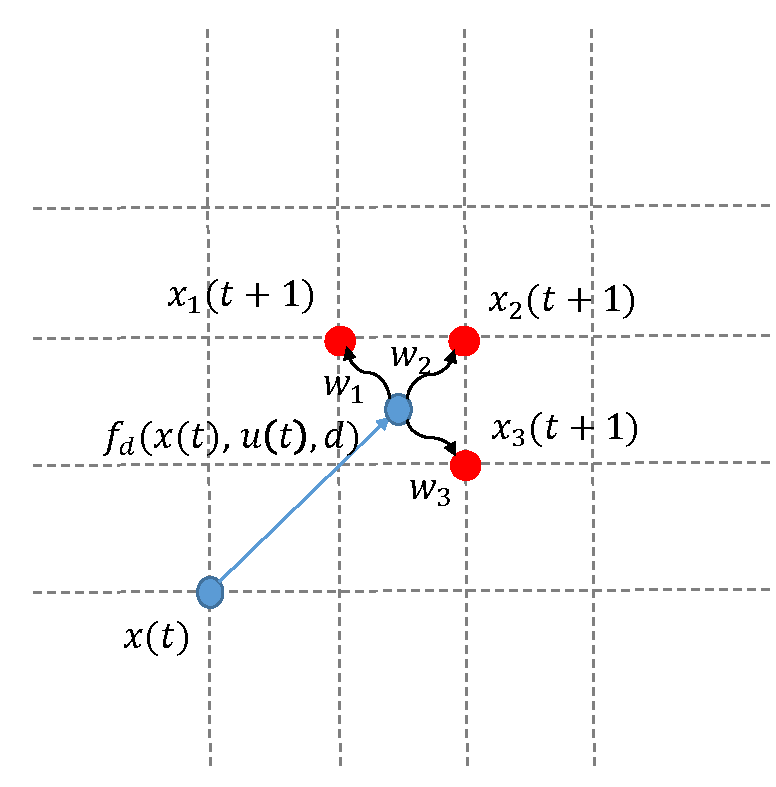
\includegraphics[width=0.40\textwidth]{interpolation.pdf}
				\label{fig:interpolation}}
        \subfloat[Agregation probabilities]{
				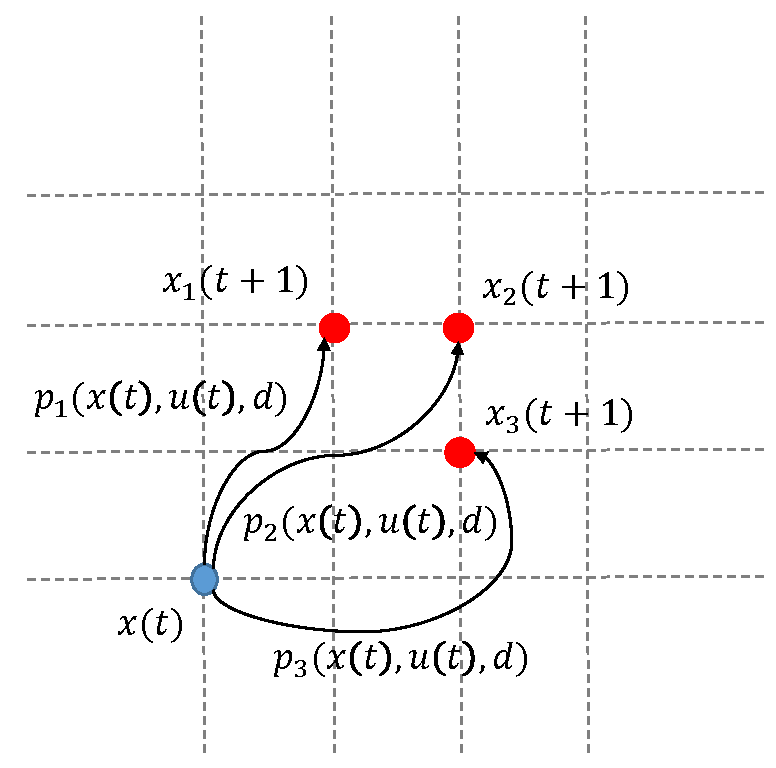
\includegraphics[width=0.40\textwidth]{Probinterpolation.pdf}
				\label{fig:Probinterpolation}}
       \caption{Approximation of the cost-to-go: two interpretations }
			\label{fig:aaa}
			\vspace{-10pt}
\end{figure}
%

An evenly spaced grid of nodes is used to represent the state space. The discrete state evolution of the system is computed by projecting in the future with a small time step $\Delta t$, using the continuous time EoM of the robotic system:
%
\begin{align}
\boldsymbol{x}(t+1) &= f_d( \boldsymbol{x}(t) , \boldsymbol{u}(t) , \boldsymbol{d}(t) ) \\
\left[ \begin{array}{c} 
	\dot{\vec{q}}(t+1) \\ \vec{q}(t+1)
\end{array} \right] &= 
\left[ \begin{array}{c} 
	H_k^{-1} \left[ R_k \vec{\tau}(t) - \vec{c}_k( \dot{\vec{q}}(t) , \vec{q}(t))  + \vec{d}(t)  \right] \Delta t + \dot{\vec{q}}(t)  \\ \dot{\vec{q}}(t)  \Delta t + \vec{q}(t) 
\end{array} \right]
\end{align}
%
However, the equations of motion of the system can lead the system to a future state that will not be exactly on a grid point corresponding to a discrete node, see Fig. \ref{fig:interpolation}. To solve this problem, the cost-to-go of the next point is computed by interpolating the cost-to-go of the neighboring grid points, based on geometric interpolation weight:
%
\begin{align}
	J(\boldsymbol{x}(t+1)) \approx \sum{ w_j J(\boldsymbol{x}_j(t+1)) }  \quad \quad \sum{ w_j  } = 1
	\label{eq:interpol}
\end{align}
%
The interpolation can also be interpreted as computing an expected value with probabilities $w_j$ of arriving on a neighboring node $j$:
%
\begin{align}
	\sum{ w_j J(\boldsymbol{x}_j(t+1)) }   &= E \left[ J(\boldsymbol{x}(t+1)) \right] \\ 
	\text{if} & \quad
	p \Big(
	\boldsymbol{x}(t+1) = \boldsymbol{x}_j 
	\; \Big| \; 
	\boldsymbol{x}(t) , \boldsymbol{u}(t) , \boldsymbol{d}(t) 
	\Big)  = w_j
	\label{eq:expectation}
\end{align}
%
Thus the value iteration updates have the form:
%
\begin{align}
	J(\boldsymbol{x}_i) \Leftarrow \operatornamewithlimits{min}\limits_{\boldsymbol{u}} 
	\left[ g(\boldsymbol{x}_i,\boldsymbol{u}) + \sum{ w_j J(\boldsymbol{x}_j(t+1))}  \right]
\end{align}
%
and the optimal control policy $\pi:\vec{x}\mapsto\vec{u}$ is computed for all nodes as:
%
\begin{align}
\pi(\boldsymbol{x}_i) = \operatornamewithlimits{argmin}\limits_{\boldsymbol{u}} 
\left[ g(\boldsymbol{x}_i,\boldsymbol{u}) + \sum{ w_j J(\boldsymbol{x}_j(t+1))}  \right]
\end{align}
%
or equivalently with the probabilistic view:
%
\begin{align}
J(\boldsymbol{x}_i) \Leftarrow \operatornamewithlimits{min}\limits_{\boldsymbol{u}} E \Big[ g(\boldsymbol{x}_i,\boldsymbol{u}) + J(\boldsymbol{x}_j(t+1))  \Big] \\
\pi(\boldsymbol{x}_i) = \operatornamewithlimits{argmin}\limits_{\boldsymbol{u}}  E \Big[ g(\boldsymbol{x}_i,\boldsymbol{u}) + J(\boldsymbol{x}_j(t+1))  \Big]
\end{align}



As illustrated at Figure. \ref{fig:Probinterpolation}, this scheme can also be interpreted as aggregating the continuous space state into discrete nodes with the weight factors corresponding to aggregation probabilities. Hence, the problem that is solved corresponds to a stochastic shortest path problem. Knowledge regarding stochastic distribution of disturbances could be included easily with this formulation. However here, disturbances are fixed to their expected value of zero, the certainty equivalence assumption \cite{bertsekas_dynamic_2000}. Even if the uncertainty of the system is not modeled directly, the interpolation scheme has an effect equivalent to including a disturbance leading to an uncertainty on the state evolution of roughly the size of the grid.


%\subsubsection{Termination conditions}
%\label{sec:TerminationCondtions}
%
%In order to guarantee the good behavior of the value iteration scheme, nodes close to the goal state are aggregated into a big cost free and absorbing termination node.  Moreover, when the equations of motion for a given state and control lead to out-of-bound states, it is considered that the system reach with a very large cost an artificial termination node with probability one. Since it is clear from the physics that there exist proper policies that can reach the termination node, and the cost is positive definite (for both the quadratic and minimum time cost functions) it is also clear that any improper policy will be associated to an infinite cost for an infinite horizon. Thus, given those conditions value iteration algorithm is guarantee to converge to the optimal cost-to-go for any initial conditions.

\subsection{Example systems}

Numerical results of feedback policy to reach a fixed-target are presented for two simple robotics system using VGA. The first system, see Fig. \ref{fig:vi_sys1}, is a single-axis linear actuator with two gear-ratios, the output dynamic is considered to be a linear mass-damper and rotor-velocity saturations are included. The second system, see Fig. \ref{fig:vi_sys2}, is a non-linear inverted pendulum with no rotor-velocity saturation. 
%
\begin{figure}[htp]
        \centering
				\subfloat[Linear mass-damper]{
				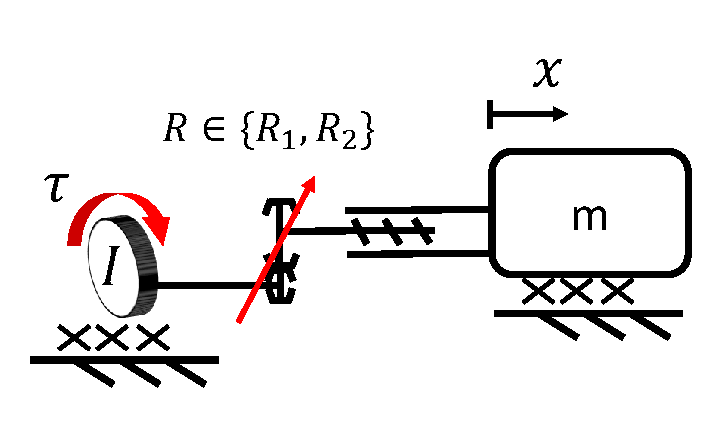
\includegraphics[width=0.40\textwidth]{vi_sys1.pdf}
				\label{fig:vi_sys1}}
				\hspace{+5pt}
        \subfloat[Inverted pendulum]{
				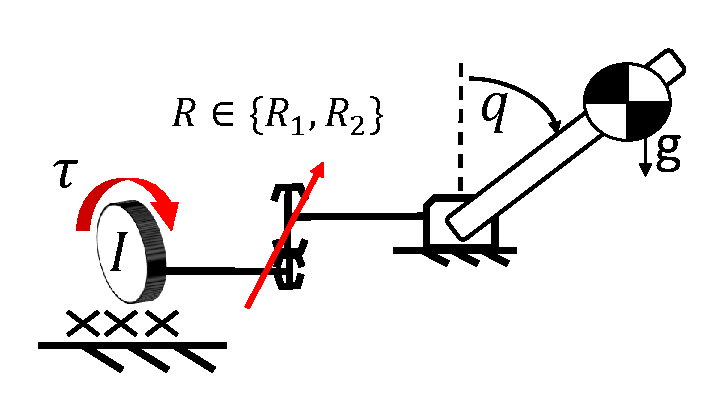
\includegraphics[width=0.40\textwidth]{vi_sys2.pdf}
				\label{fig:vi_sys2}}
       \caption{Two studied robotic systems}
			\label{fig:studiedsys}
\end{figure}
%

\subsection{Implementation}
\label{sec:Methodology}

The discretization parameters used are as follow: the state space is discretized into a 101 x 101 grid (101 equally spaced positions and 101 equally spaced speed values) leading to 10201 possible nodes, the actuator torque is discretized into 21 possible torque values, leading to a total of 42 possible control actions including the gear ratio selection. The state transition is computed using a time discretization of $\Delta t$ = 0.05 sec. The interpolation weights are computed using a bivariate spline approximation. The value iterations are stopped manually when the maximum difference between $J_k$ and $J_{k+1}$ are many orders of magnitude smaller than the variations of $J$ across the state space. The computation takes on average 200-500 iterations and 2-5 minutes.

%\subsection{Reinforcement Learning}
%
%\subsubsection{Q-Learning}
%
%Next, the Q-Learning algorithm is implemented. While here in this project we have access to the model of the system, this approach would be advantageous in a real context because we could use it directly on a prototype without having a model of the robot. 
%
%The Q-learning update is:
%\begin{align}
	%Q( \boldsymbol{x} , \boldsymbol{u} ) &= Q( \boldsymbol{x} , \boldsymbol{u} ) + \alpha \left[ g(\boldsymbol{x} , \boldsymbol{u}) + \lambda J( \boldsymbol{x}_{(t+1)}  )  -  Q( \boldsymbol{x} , \boldsymbol{u} ) \right] \\
	%J( \boldsymbol{x}  ) &= \min_{\boldsymbol{u}} Q( \boldsymbol{x}, \boldsymbol{u} )
   %\end{align}
   %
%This update is conducted for each set of $\left[ \boldsymbol{x}_{(t)}  , \boldsymbol{u}_{(t)}  , \boldsymbol{x}_{(t+1)}   \right]$ collected using simulated experiments. The controller used for the experiment is $\epsilon$-greedy, i.e. $\epsilon$ fraction of the time it picks a random action, else it is using the optimal action so far ( $ u(\boldsymbol{x})  = arg\min_{\boldsymbol{u}} Q( \boldsymbol{x}, \boldsymbol{u} ) $ ). The training is done as follow: first conduct a 10 sec simulation with the $\epsilon$-greedy controller, then go through the collected state-action pairs and conduct a Q-values update for each data-point, then start again.



\subsection{Numerical results}

\subsubsection{System 1 - Linear mass-damper robot}
Fig. \ref{fig:J} to \ref{fig:u1} illustrate the numerical results for system 1. Three different cost functions are explored, a quadratic cost function, a minimum time cost and minimum energy case which is simply a special case of the quadratic cost where weight are sets to drastically penalize control inputs over state error. The absence of color indicates states with no solution (a constraint will be violated for any possible control actions). Fig. \ref{fig:phase_plane} shows the closed loop behavior of the system in the phase plane when the optimal policy is applied.
%
\begin{figure}[p]
				\vspace{-2pt}
        \centering
				\subfloat[Minimum time]{
        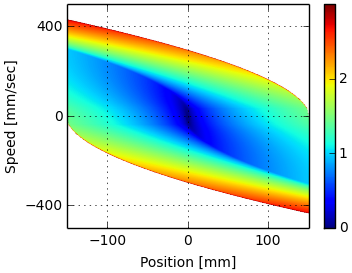
\includegraphics[width=0.31\textwidth]{Jt.png}
				\label{fig:J_time}}
        \subfloat[Quadratic cost]{
				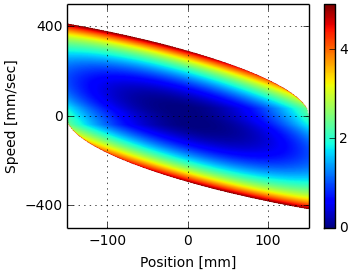
\includegraphics[width=0.31\textwidth]{Jq.png}%J_LQR.png
				\label{fig:J_LQR}}
				\subfloat[Minimum energy]{
				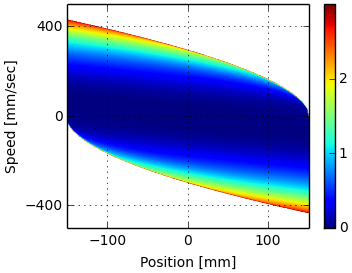
\includegraphics[width=0.31\textwidth]{Je.png}
				\label{fig:J_energy}}
        \caption[Optimal cost-to-go]{Optimal cost-to-go $J^*$}\label{fig:J}
\end{figure}
%
\begin{figure}[p]
				\vspace{-2pt}
        \centering
				\subfloat[Minimum time]{
        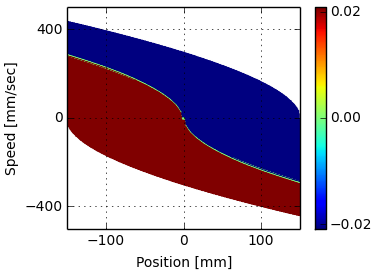
\includegraphics[width=0.31\textwidth]{u1t.png}
				\label{fig:u0_time}}
        \subfloat[Quadratic cost]{
				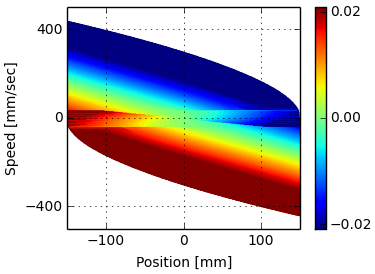
\includegraphics[width=0.31\textwidth]{u1q.png}
				\label{fig:u0_LQR}}
				\subfloat[Minimum energy]{
				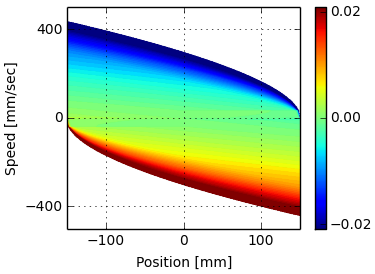
\includegraphics[width=0.31\textwidth]{u1e.png}
				\label{fig:u0_energy}}
        \caption[Optimal policy for the continuous torque command]{Optimal policy for the continuous torque command $\tau$ [Nm]}\label{fig:u0}
\end{figure}
%
\begin{figure}[p]
				\vspace{-2pt}
        \centering
				\subfloat[Minimum time]{
        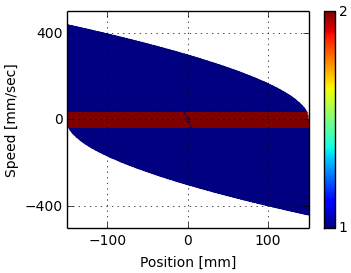
\includegraphics[width=0.31\textwidth]{u2t.png}
				\label{fig:u1_time}}
        \subfloat[Quadratic cost]{
				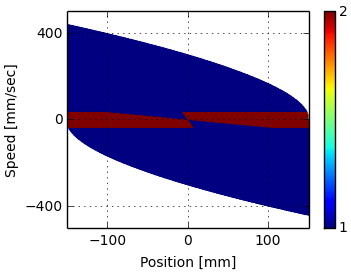
\includegraphics[width=0.31\textwidth]{u2q.png}
				\label{fig:u1_LQR}}
				\subfloat[Minimum energy]{
				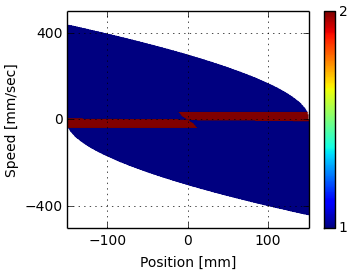
\includegraphics[width=0.31\textwidth]{u2e.png}
				\label{fig:u1_energy}}
        \caption[Optimal policy for the gear-ratio mode selection]{Optimal policy for the gear-ratio mode selection $k$}\label{fig:u1}
\end{figure}
%
\begin{figure}[p]
				\vspace{-2pt}
        \centering
				\subfloat[Minimum time]{
        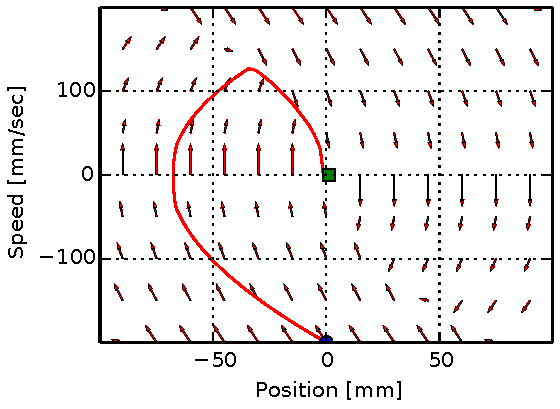
\includegraphics[width=0.31\textwidth]{ppt.pdf}
				\label{fig:phase_plane_time}}
        \subfloat[Quadratic cost]{
				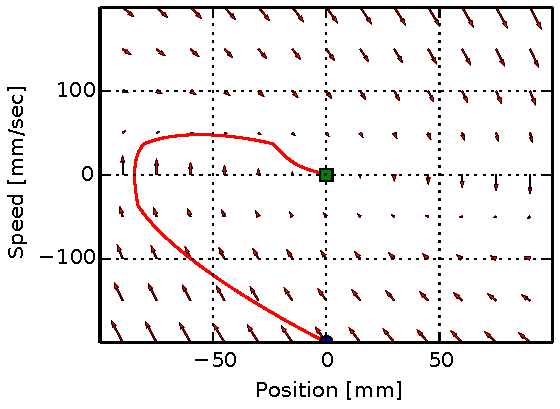
\includegraphics[width=0.31\textwidth]{ppq.pdf}
				\label{fig:phase_plane_LQR}}
				\subfloat[Minimum energy]{
				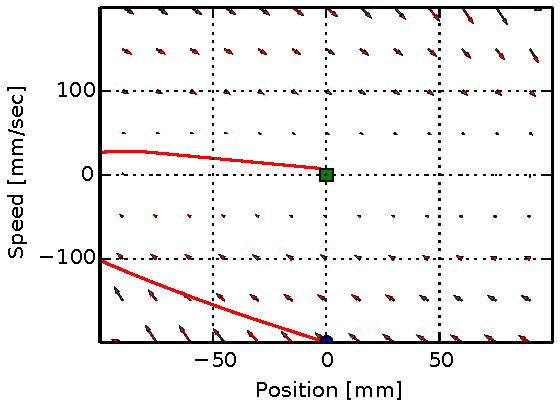
\includegraphics[width=0.31\textwidth]{ppe.pdf}
				\label{fig:phase_plane_energy}}
        \caption[Closed loop behavior in the phase plane]{Closed loop behavior with the optimal policy illustrated in the phase plane}\label{fig:phase_plane}
\end{figure}

\paragraph{Minimum time}
\label{sec:MinimumTime}
For the minimum time problem, the optimal policy is a bang-bang law for the torque and always using highly-geared mode when possible. Note that the bang-bang switching curve accounts for the fact the large gear ratio will be used during the final part of the trajectory.

\paragraph{Quadratic cost}
\label{sec:QuadraticCost}
For the quadratic cost, the gear-ratio selection optimal policy is almost as simple as the minimum time problem except for small features in quadrant II and IV. The more interesting result comes from the continuous torque control law, the gains when using the large reduction ratio are larger than those when using the small reduction ratio. This results in the controller taking action mainly at low speed when its actions have the biggest impacts on the system, and lead to a highly non-linear closed-loop behavior.

\paragraph{Minimum energy}
\label{sec:MinimumEnergy}
For the minimum energy controller, interestingly the mode selection policy is not trivial even for this simple linear model.  This shows that it does not take much complexity to have non-trivial optimal policies for hybrid systems. Here, the large reduction ratio is used almost only for braking, and in quadrant II and IV the small reduction ratio is used even at low speed to coast with low viscous resistance. Also globally the gains are much lower than the other controllers except for zones where it is necessary to use energy to stay in the state-domain. 

\subsubsection{System 2 - Inverted pendulum robot}
%
Figure \ref{fig:J2} illustrates the computed optimal cost-to-go for the inverted pendulum system for both a minimal time goal and a quadratic cost minimization. Figure \ref{fig:u02} shows the optimal torque policy and Figure \ref{fig:u12} shows the optimal gear selection policy. The resulting closed loop behavior is illustrated in the phase plane at Figure \ref{fig:phase_plane2}. Figure \ref{fig:phase_plane2} also shows closed-loop state trajectories and control inputs for a simulation starting at $q$ = -2 rad.

\begin{figure}[p]
        \centering
				\subfloat[Minimum time]{
        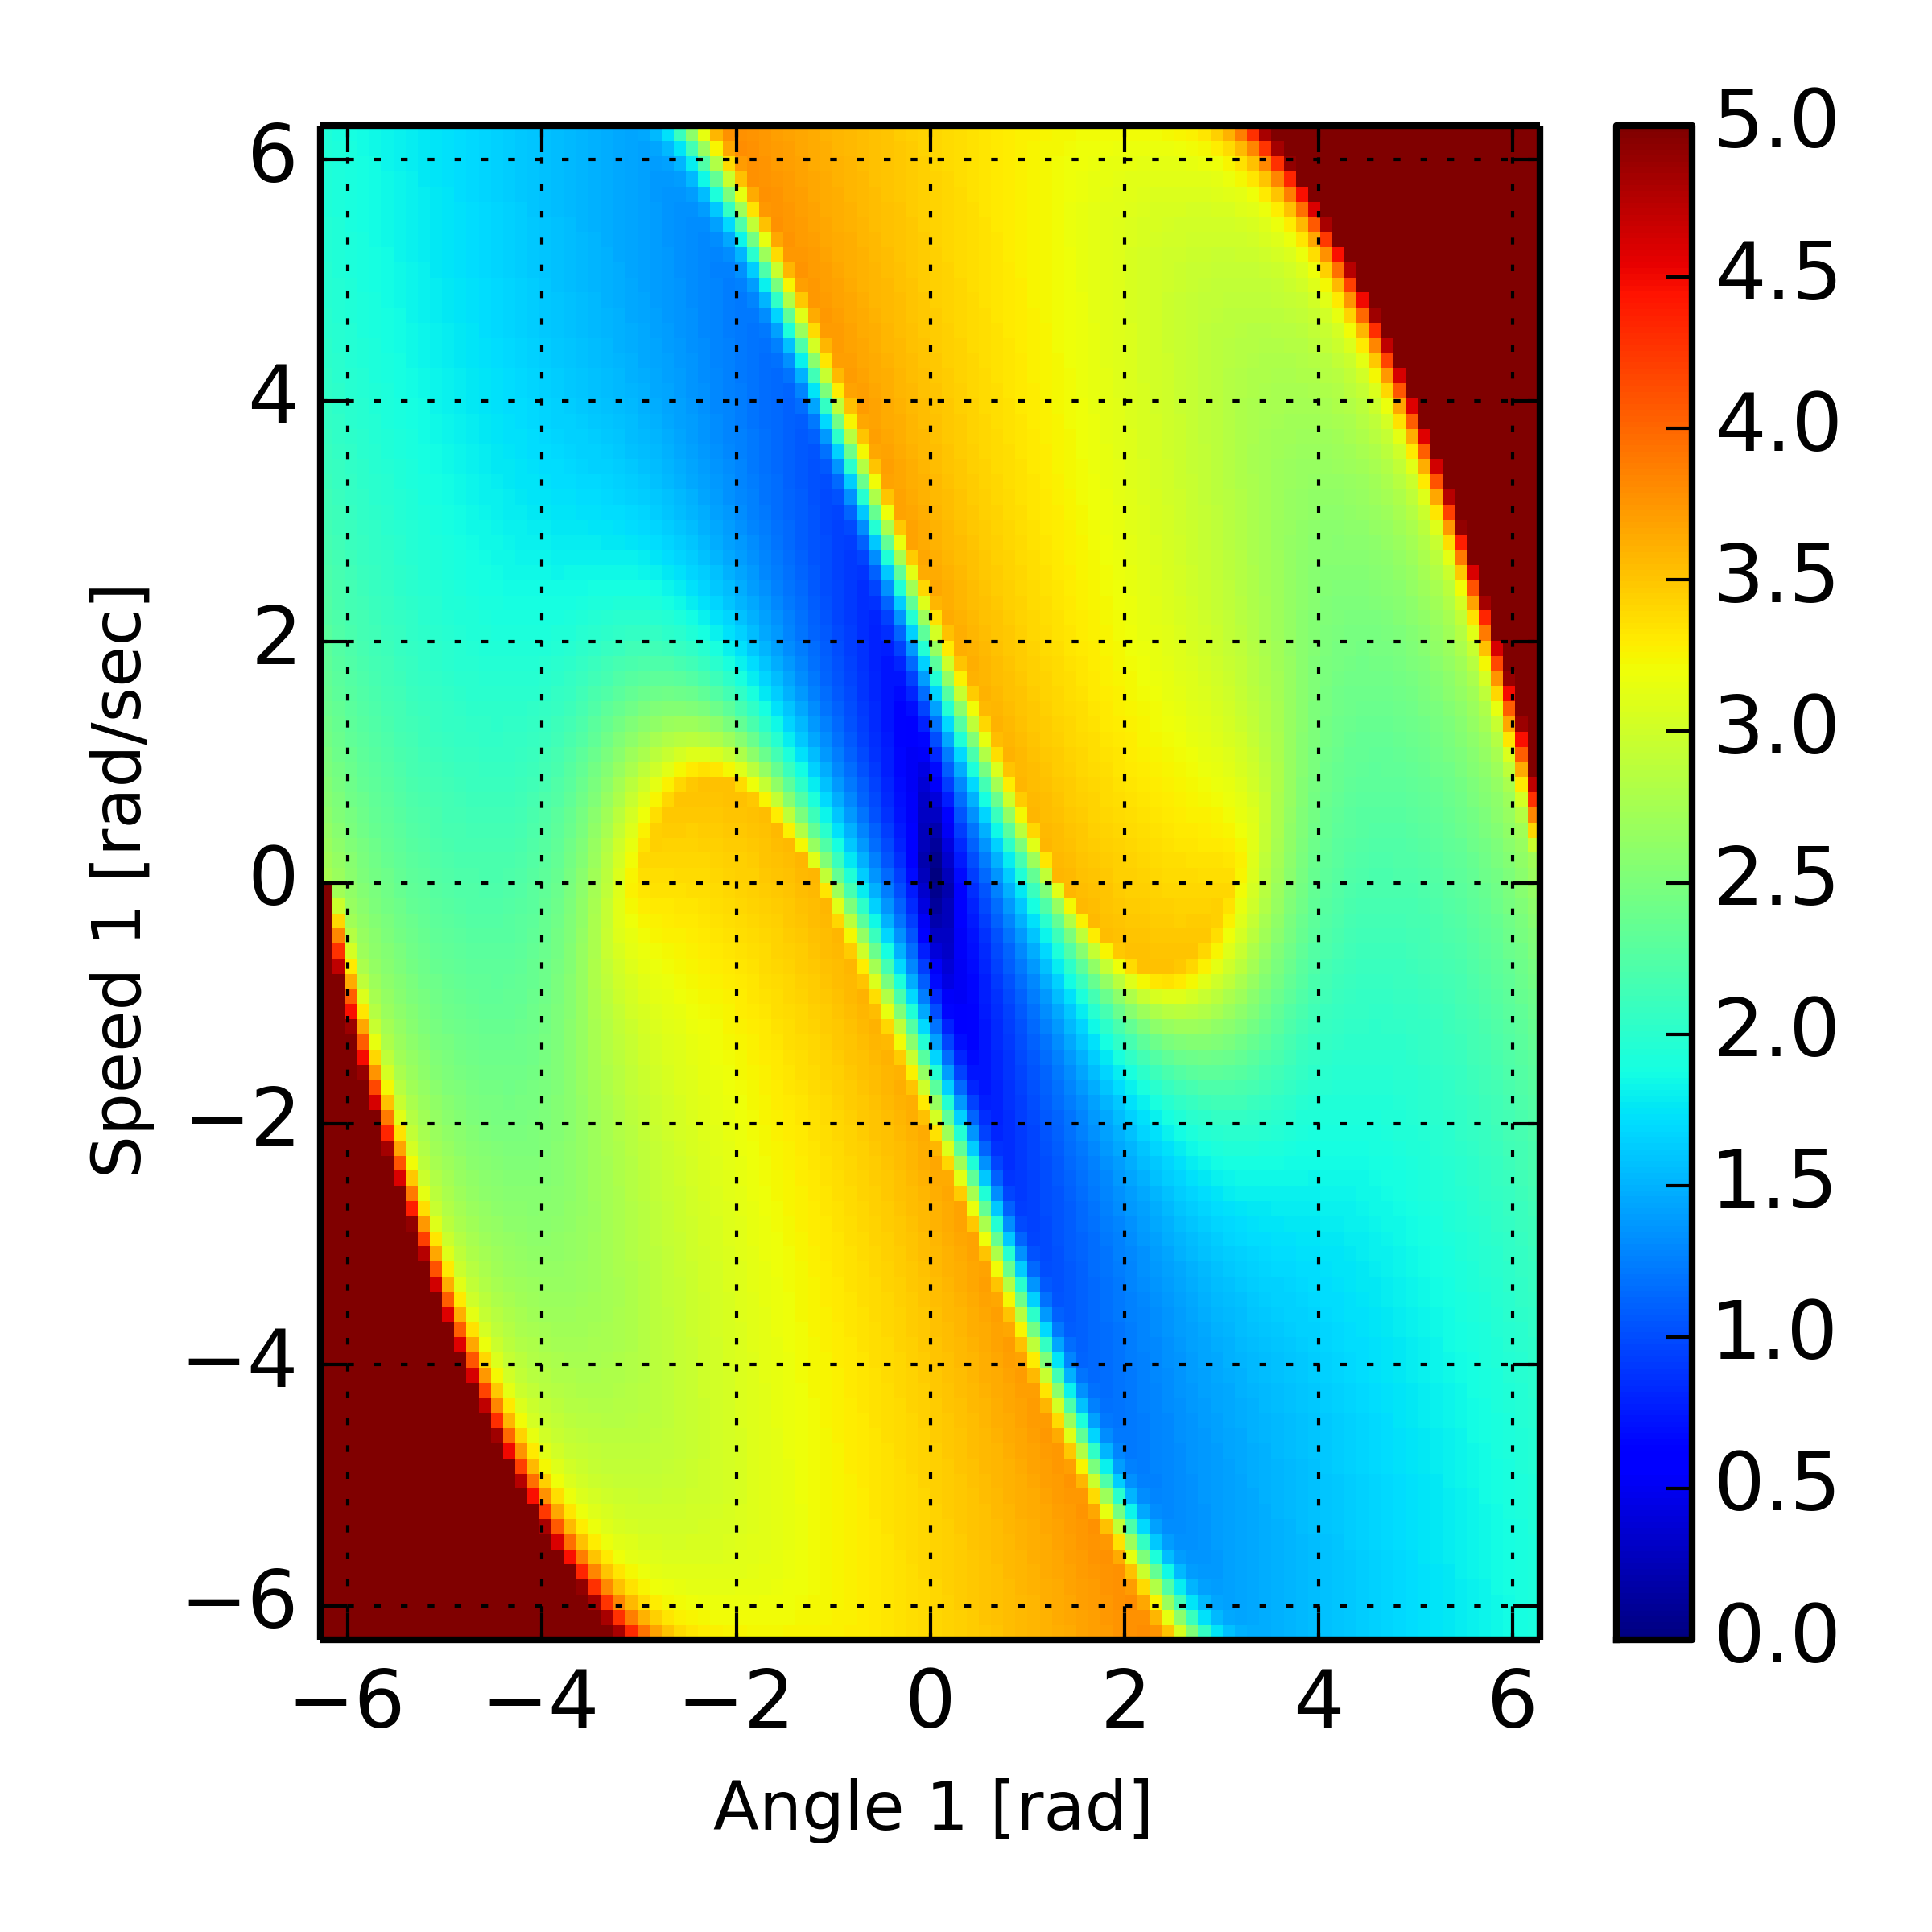
\includegraphics[width=0.48\textwidth]{J_time.png}
				\label{fig:J_time2}}
        \subfloat[Quadratic cost]{
				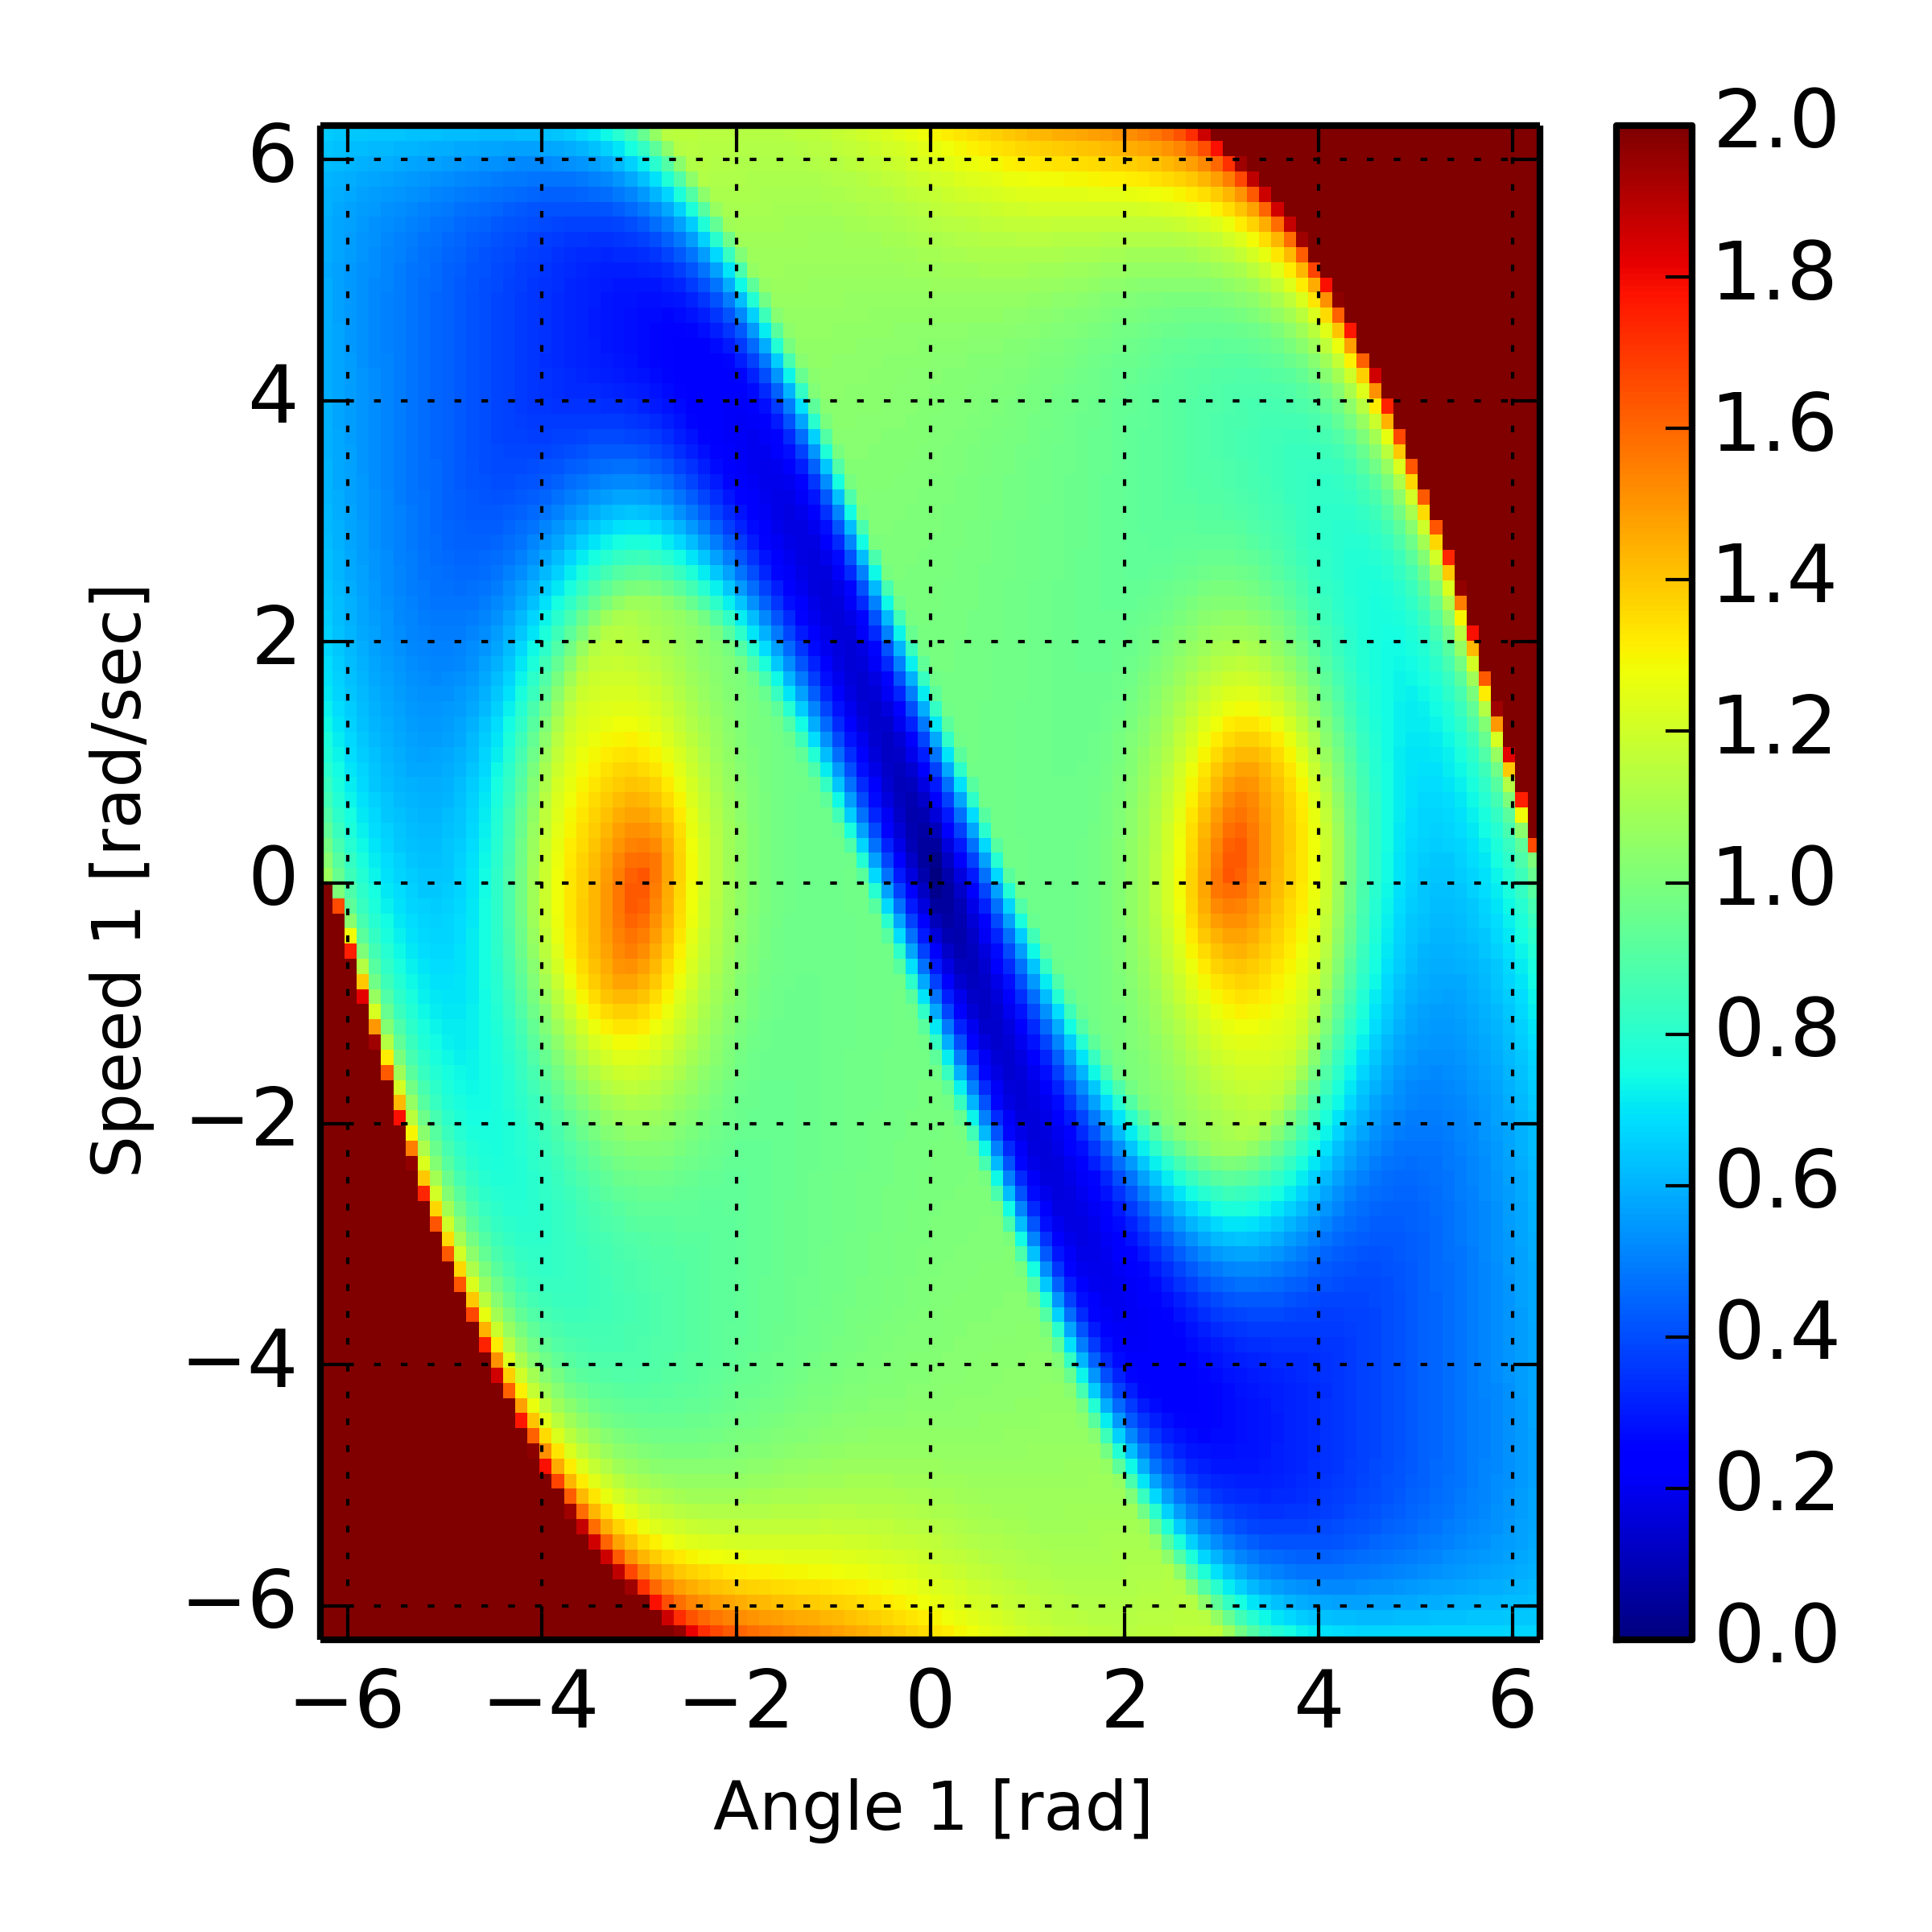
\includegraphics[width=0.48\textwidth]{J_quadratic.png}%J_LQR.png
				\label{fig:J_LQR2}}
        \caption[Optimal cost-to-go]{Optimal cost-to-go $J^*$}\label{fig:J2}
\end{figure}

\begin{figure}[p]
        \centering
				\subfloat[Minimum time]{
        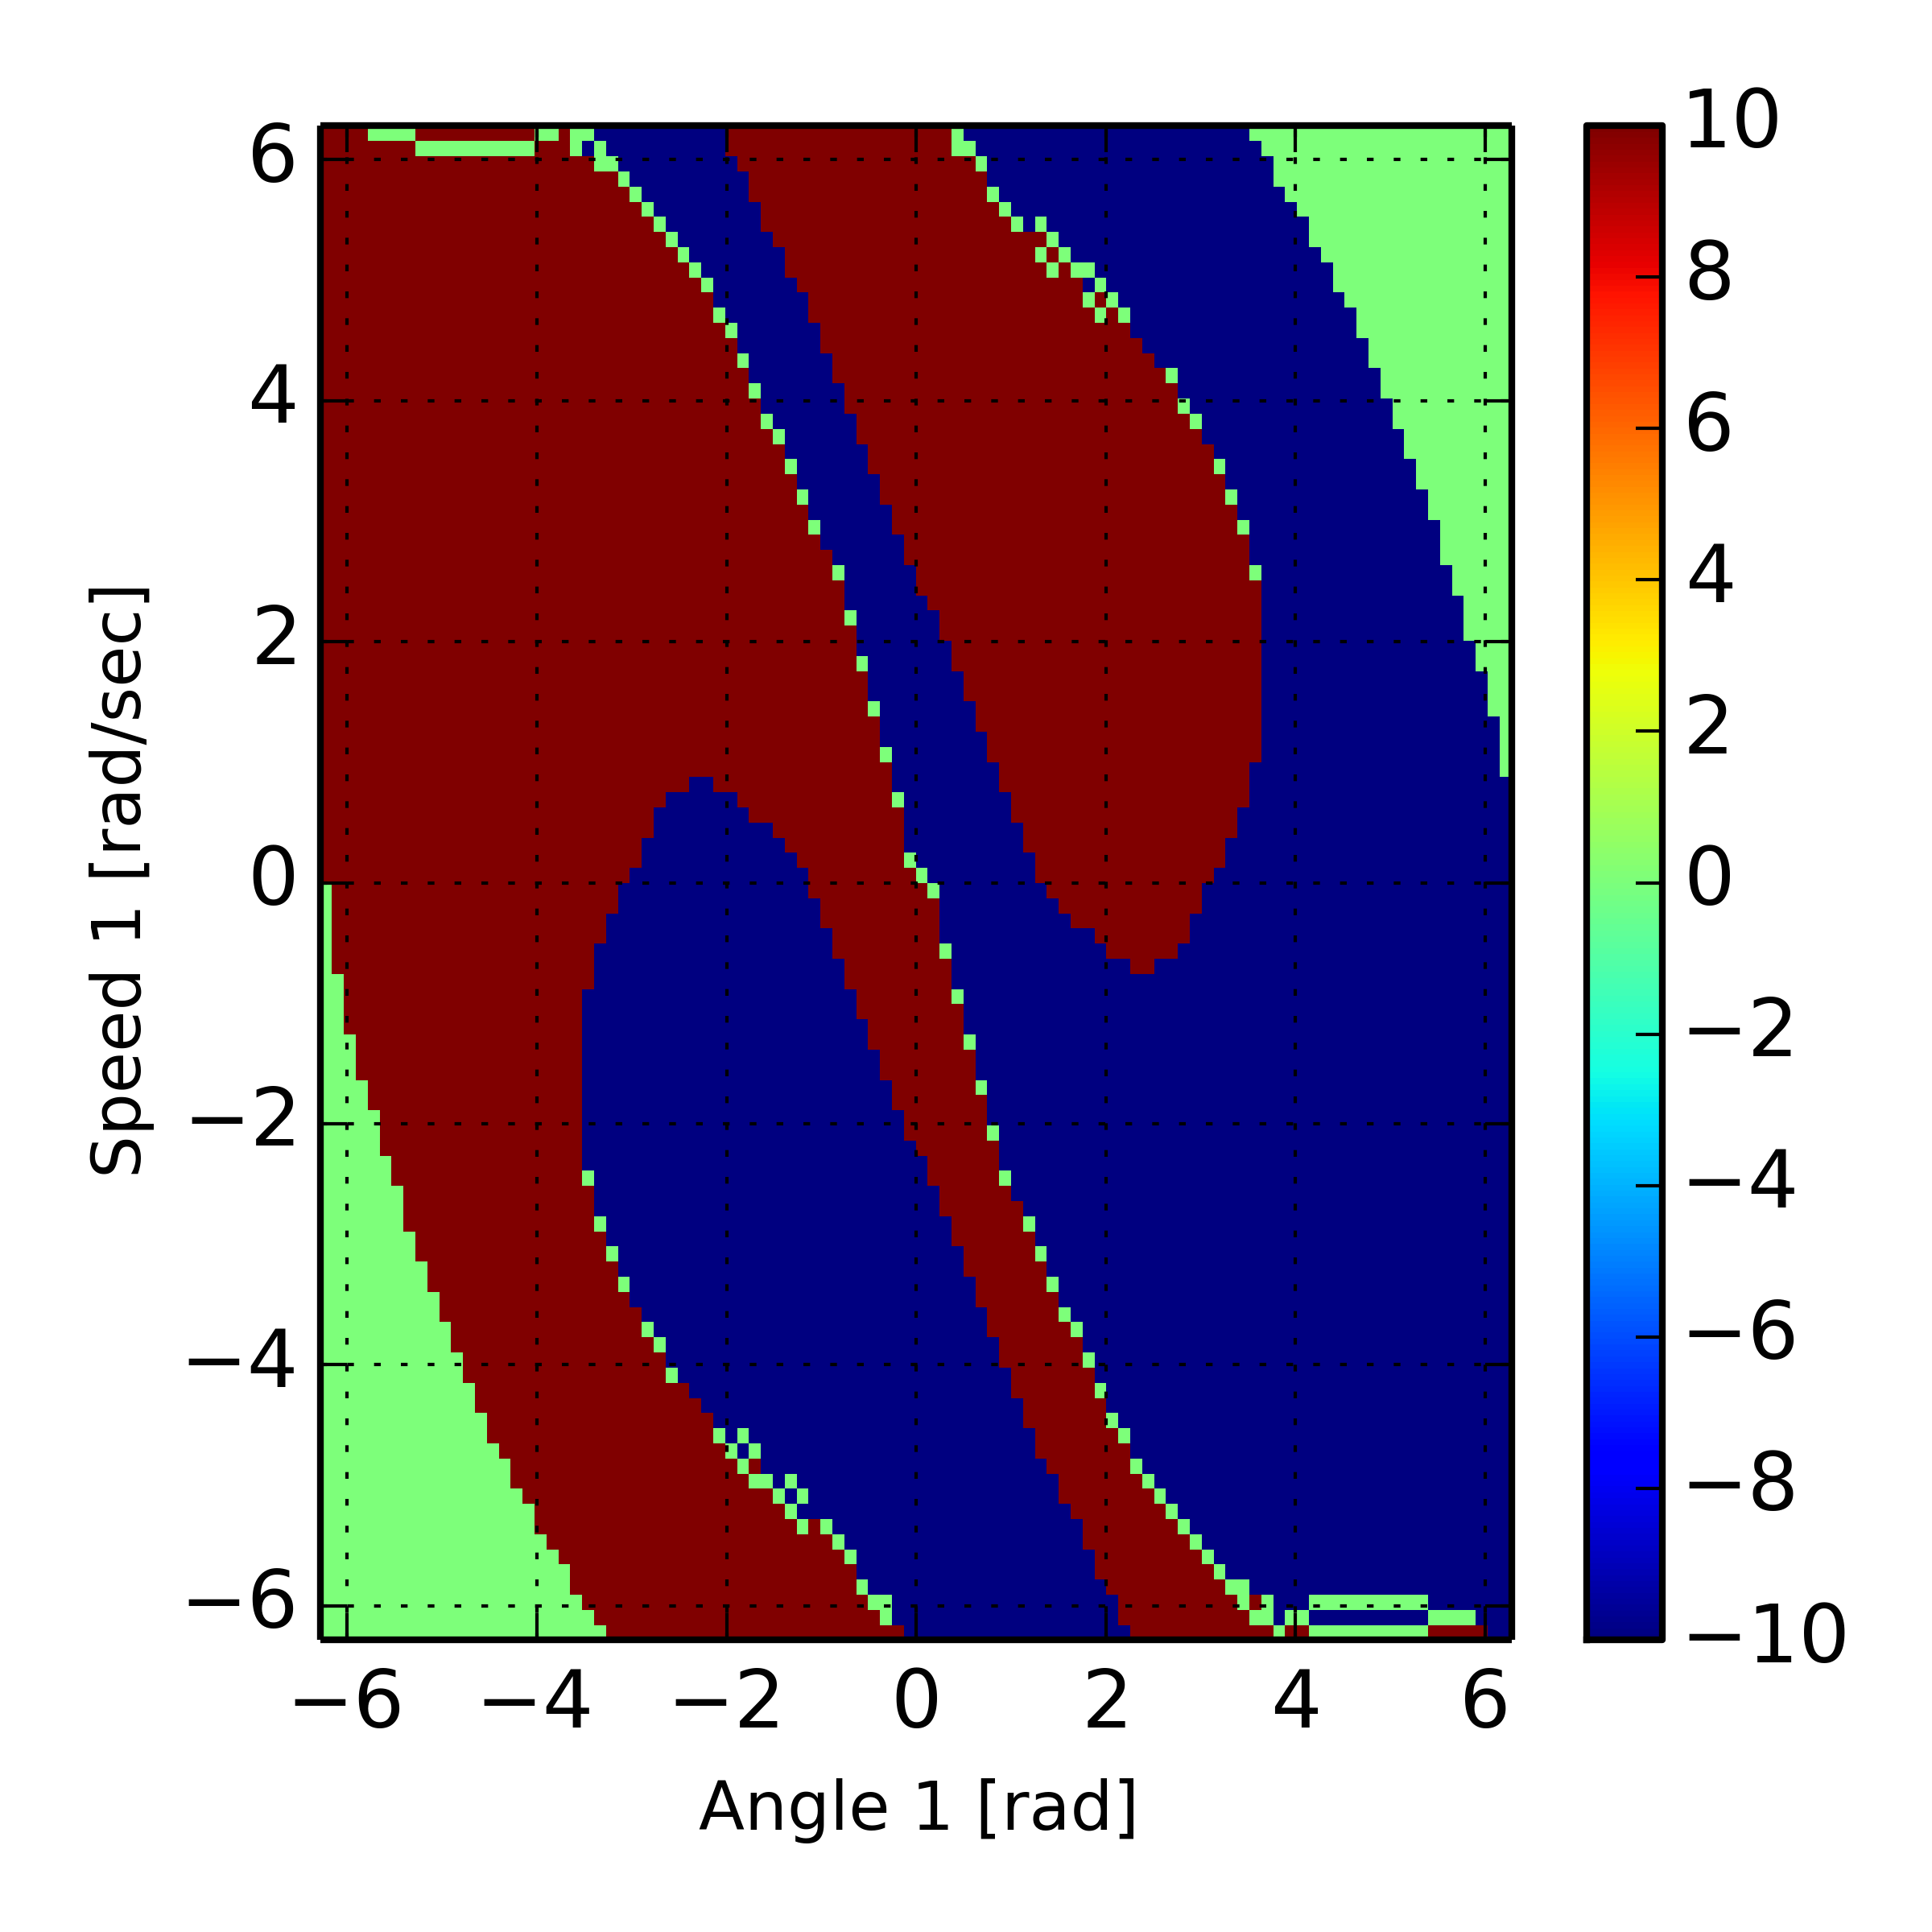
\includegraphics[width=0.48\textwidth]{u0_time.png}
				\label{fig:u0_time2}}
        \subfloat[Quadratic cost]{
				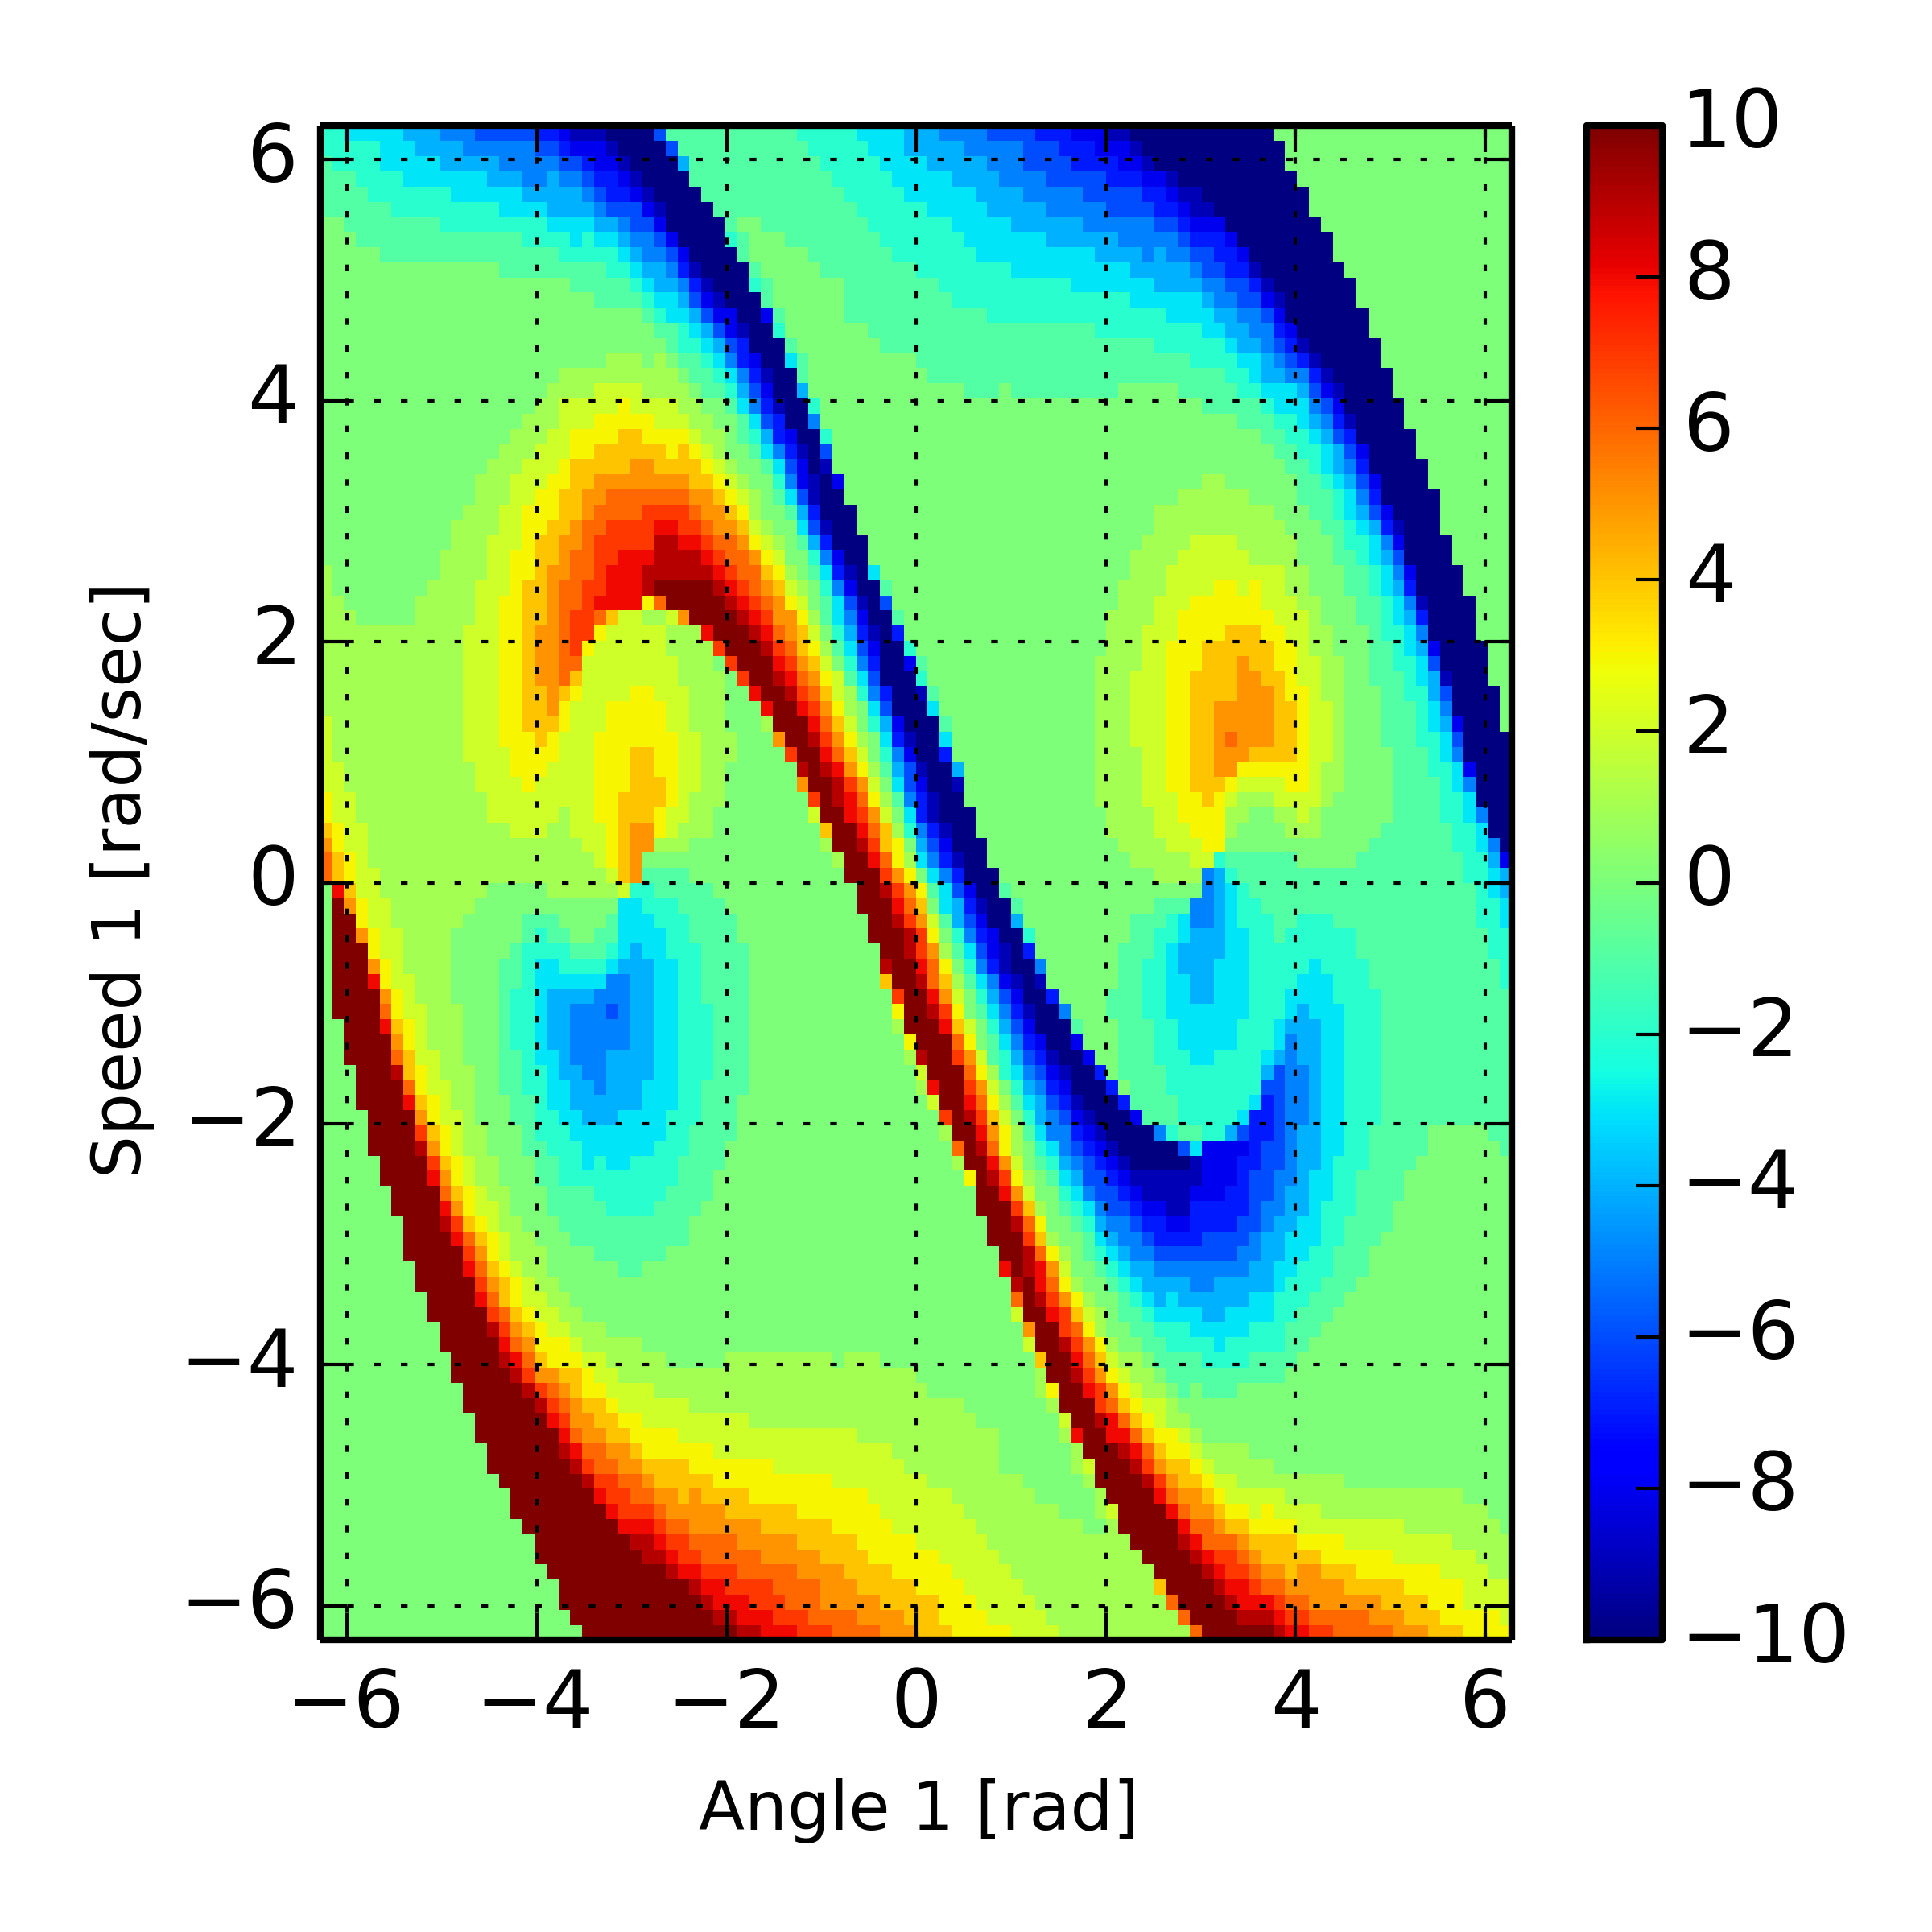
\includegraphics[width=0.48\textwidth]{u0_quadratic.png}
				\label{fig:u0_LQR2}}
        \caption[Optimal policy for the continuous torque command]{Optimal policy for the continuous torque command $\tau$ [Nm]}\label{fig:u02}
\end{figure}

\begin{figure}[p]
        \centering
				\subfloat[Minimum time]{
        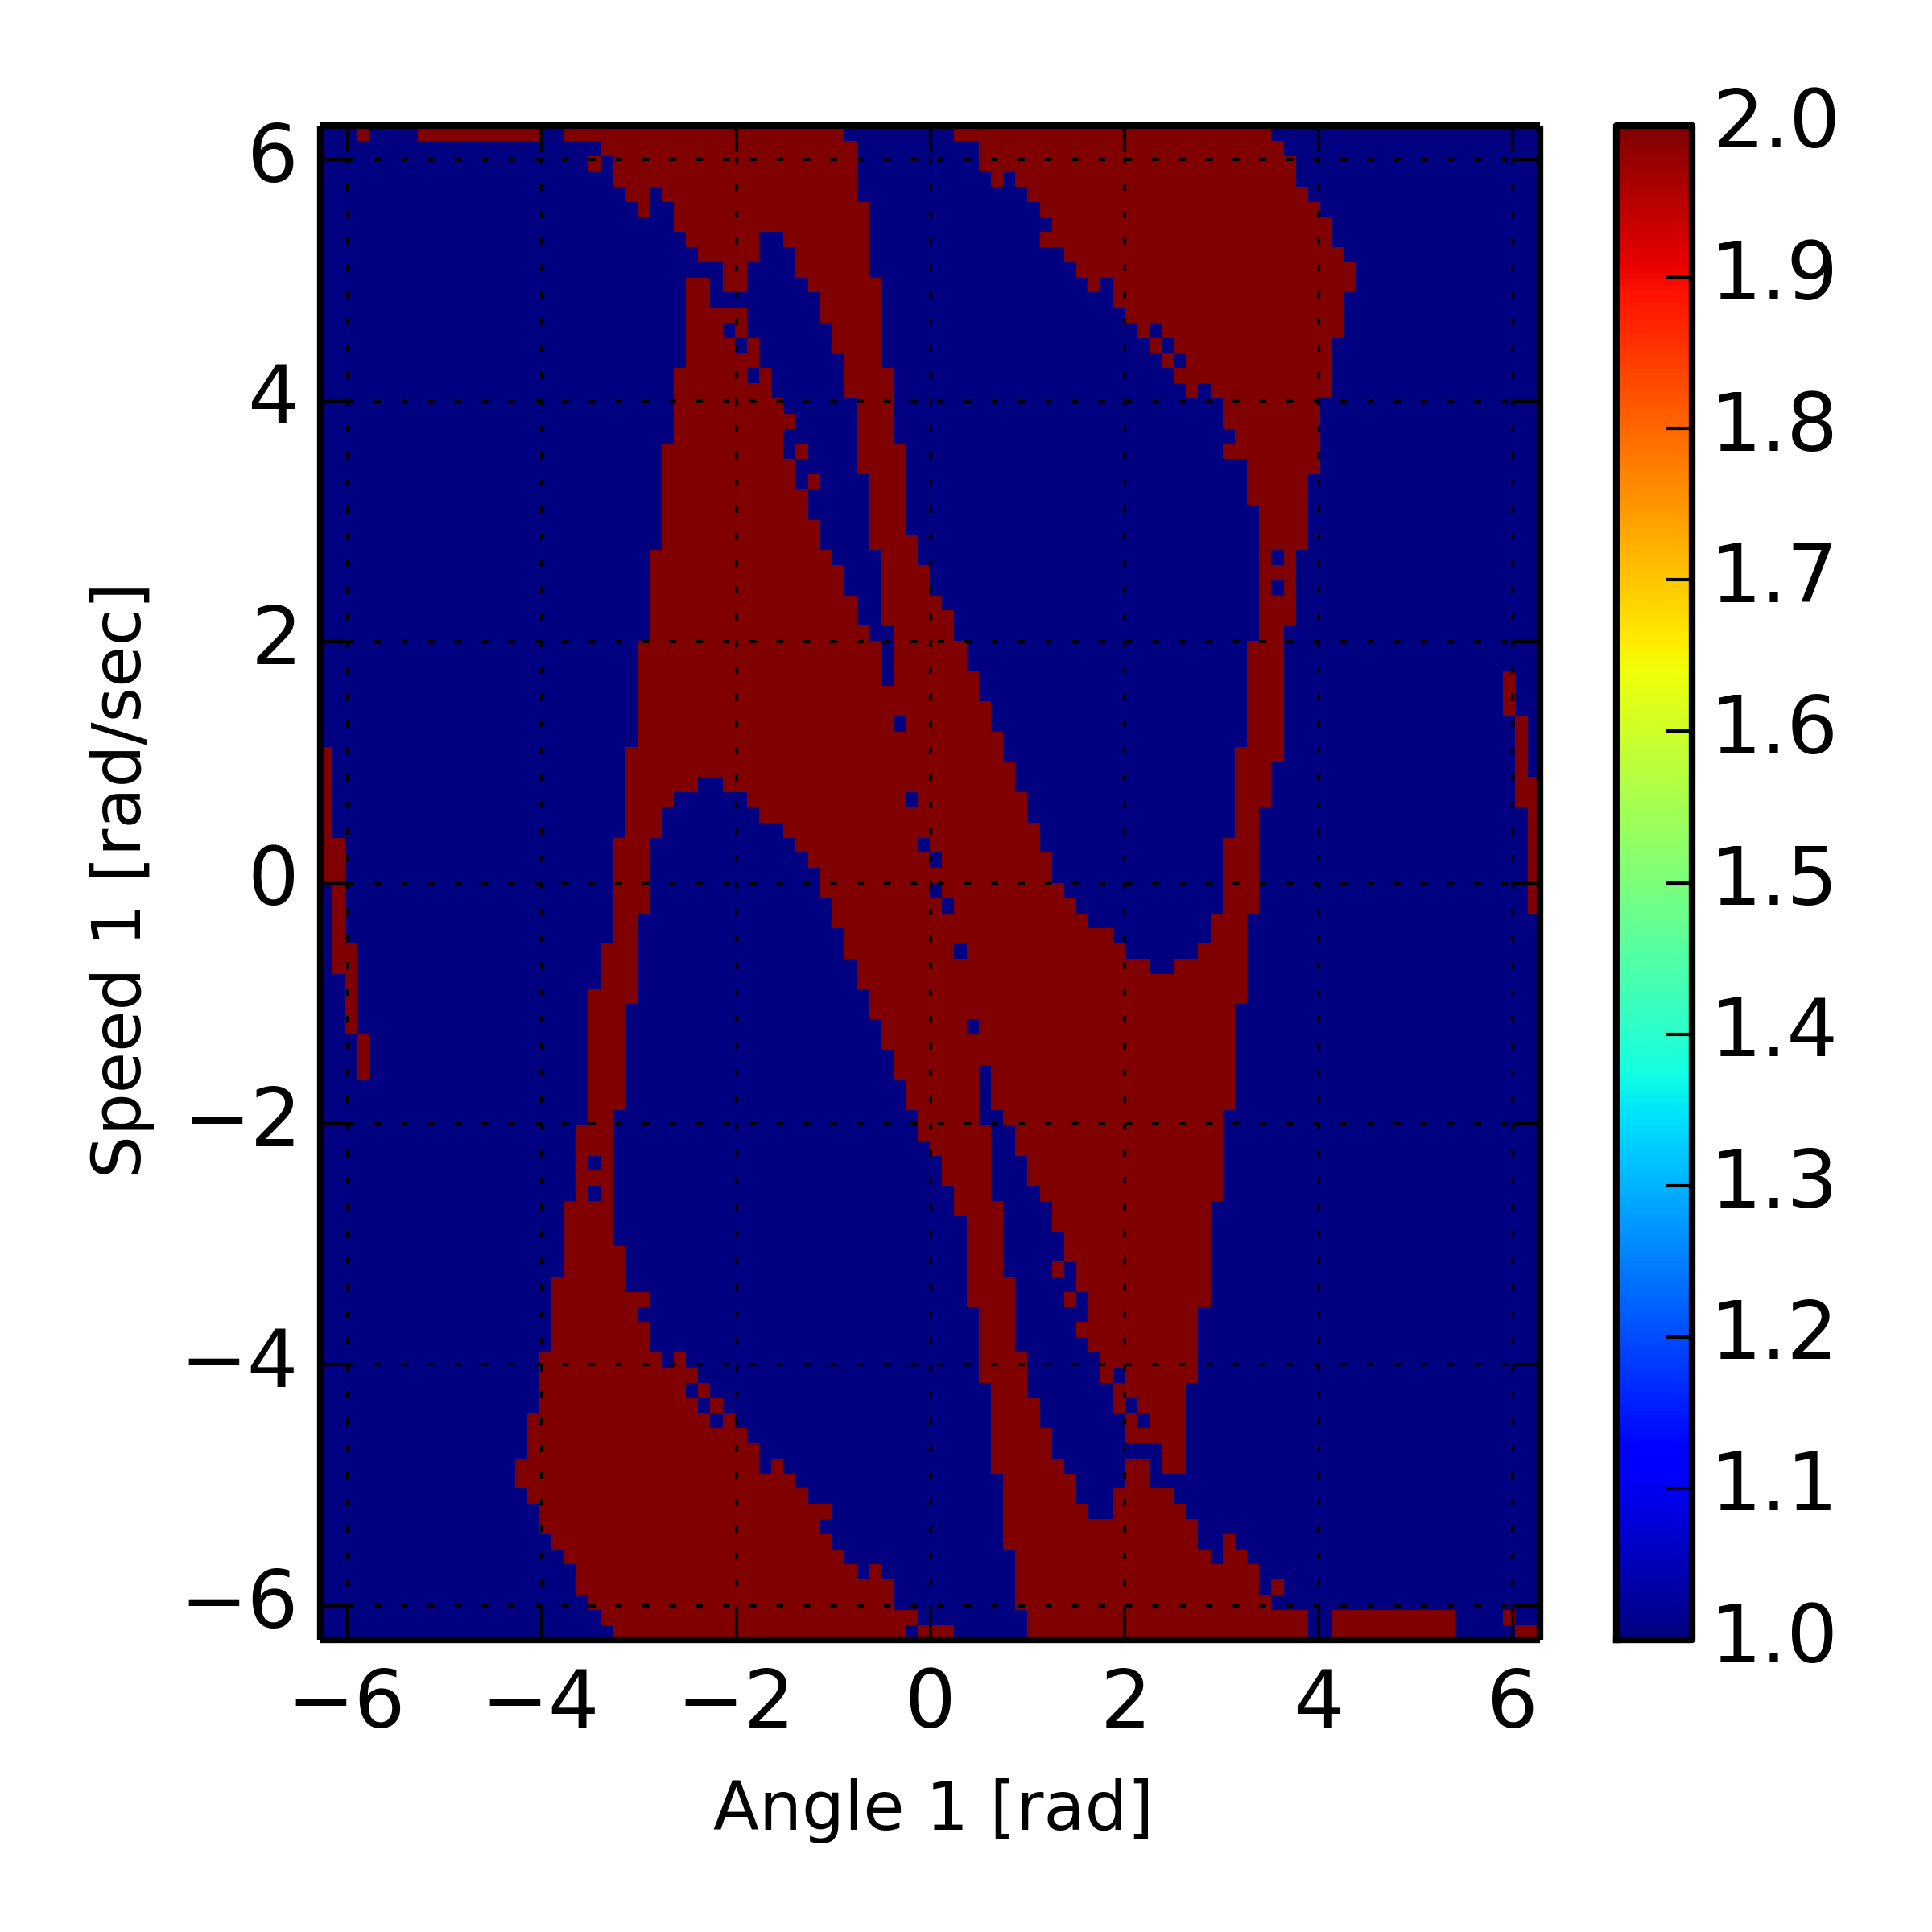
\includegraphics[width=0.48\textwidth]{u1_time.png}
				\label{fig:u1_time2}}
        \subfloat[Quadratic cost]{
				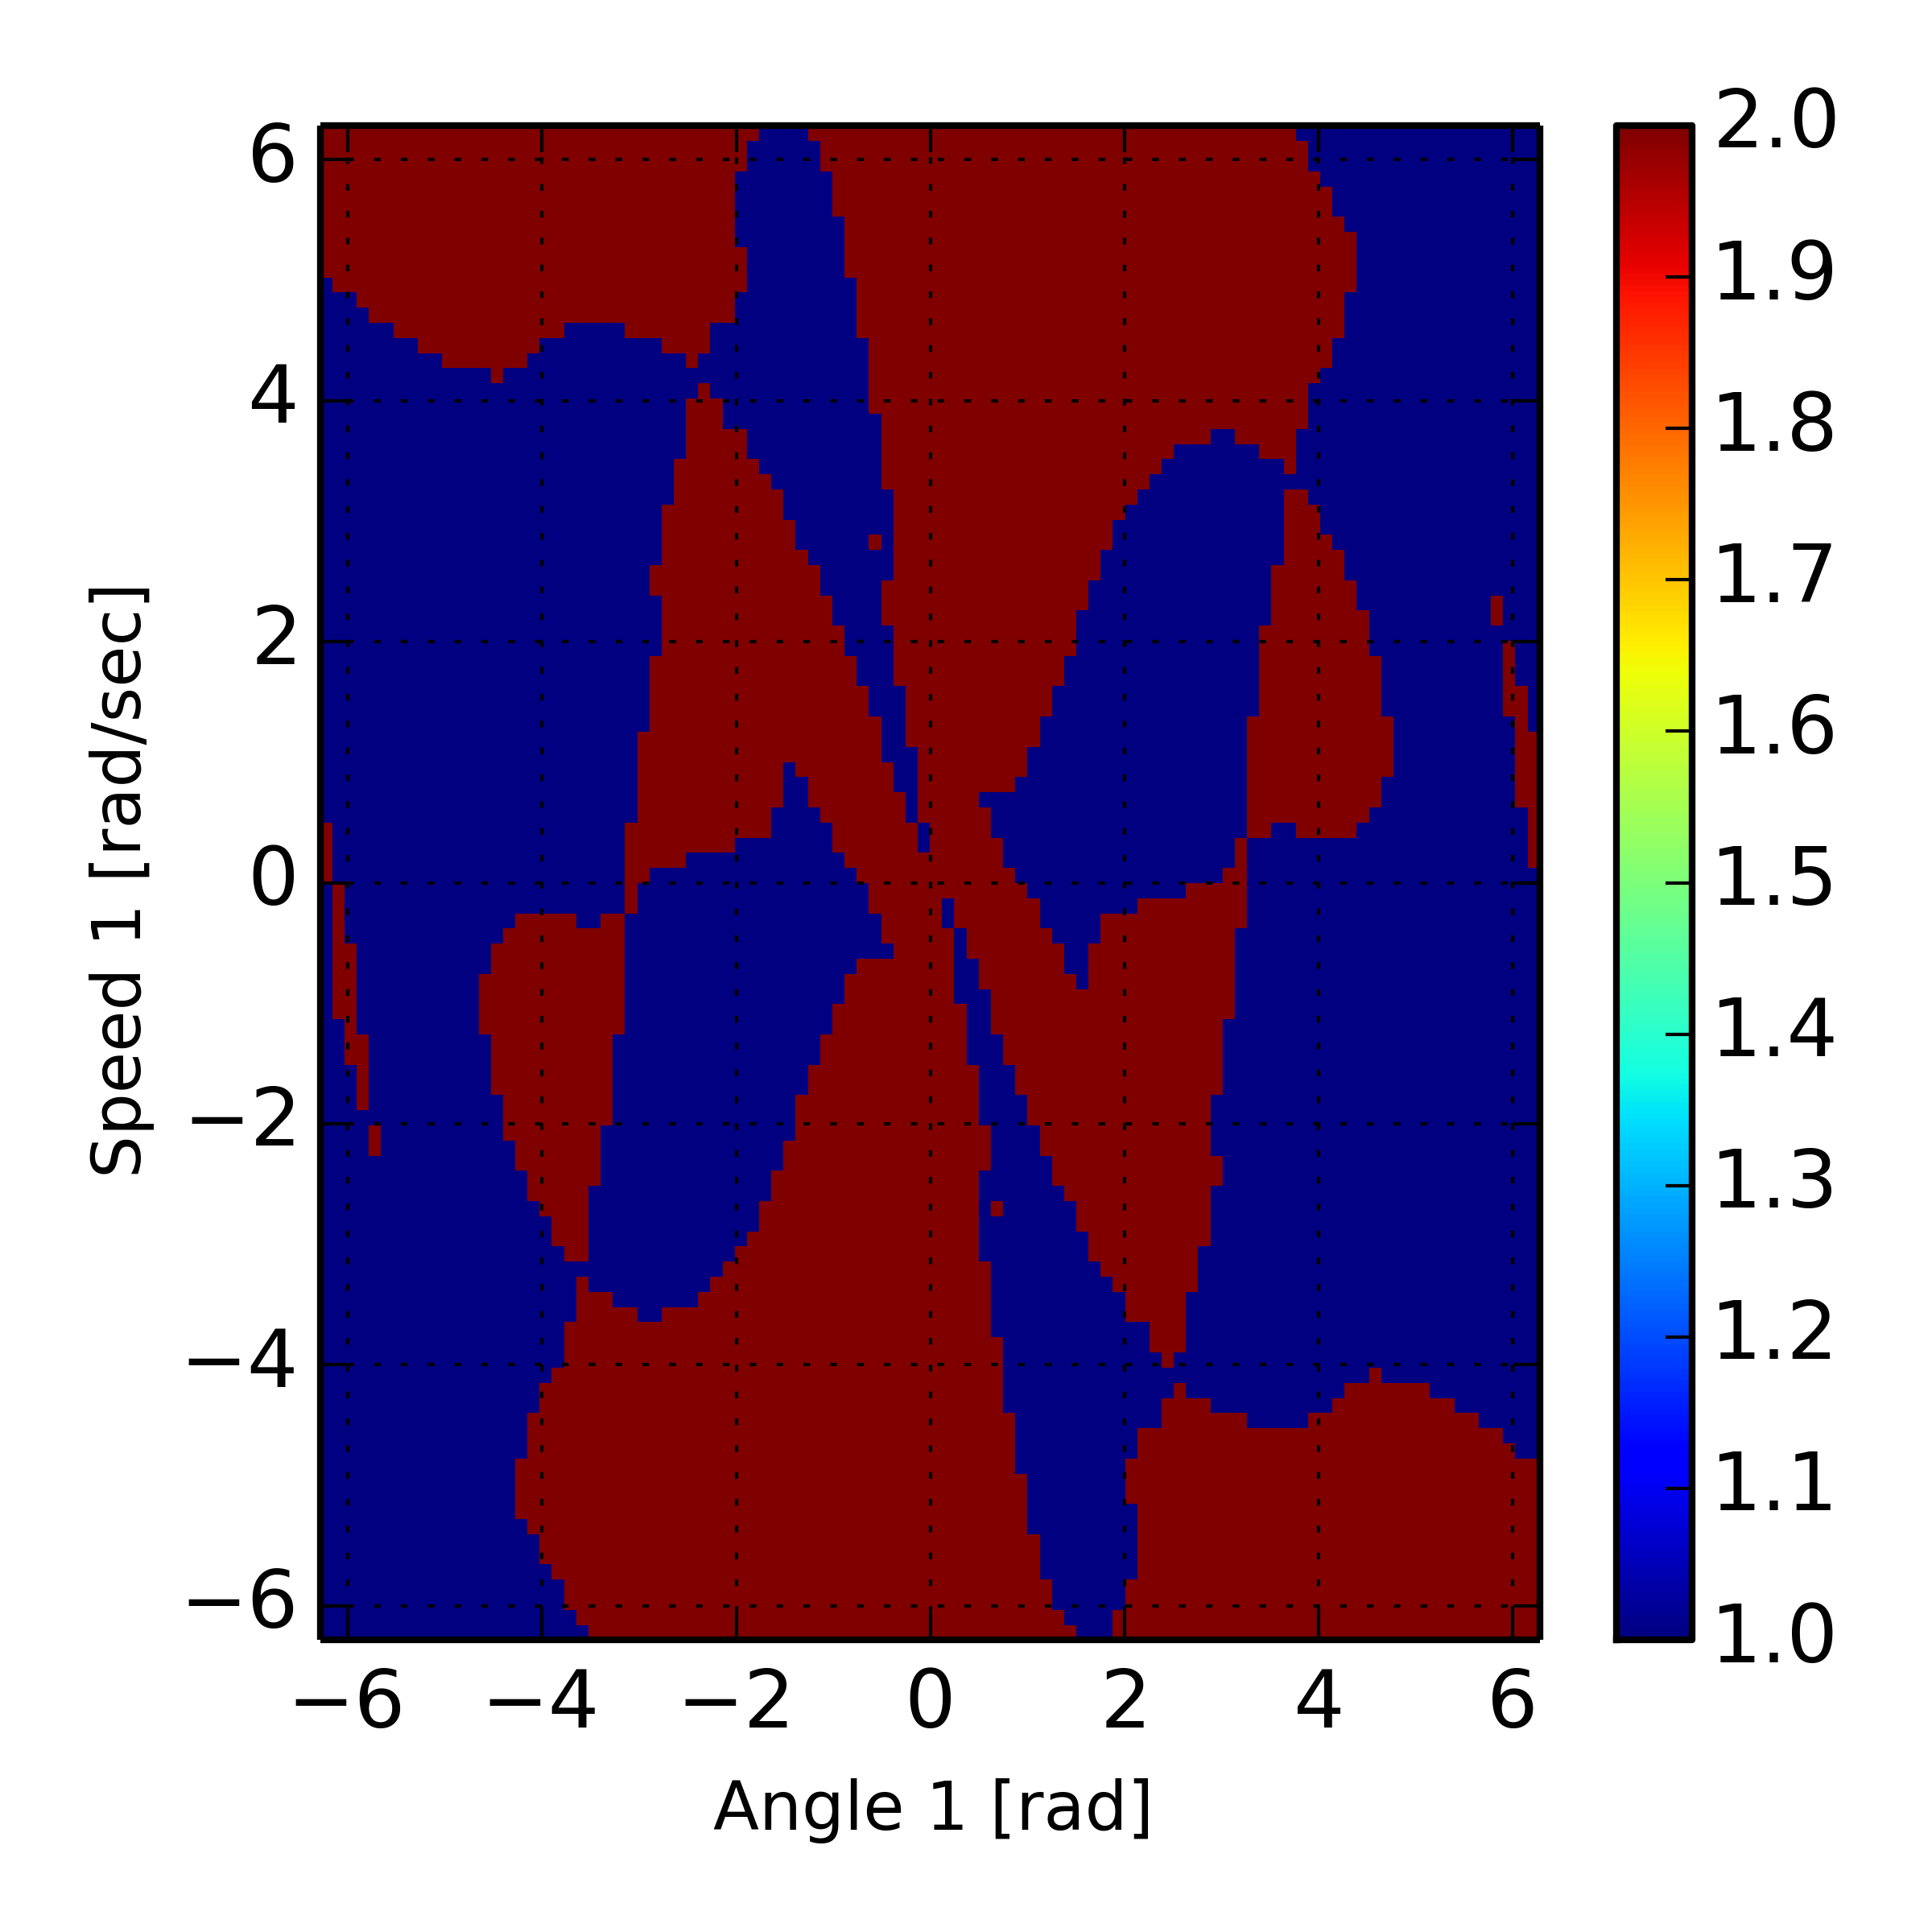
\includegraphics[width=0.48\textwidth]{u1_quadratic.png}
				\label{fig:u1_LQR2}}
        \caption[Optimal policy for the discrete gear selection]{Optimal policy for the discrete gear selection $k \in \{1,2\}$}\label{fig:u12}
\end{figure}

\begin{figure}[p]
        \centering
				\subfloat[Minimum time]{
        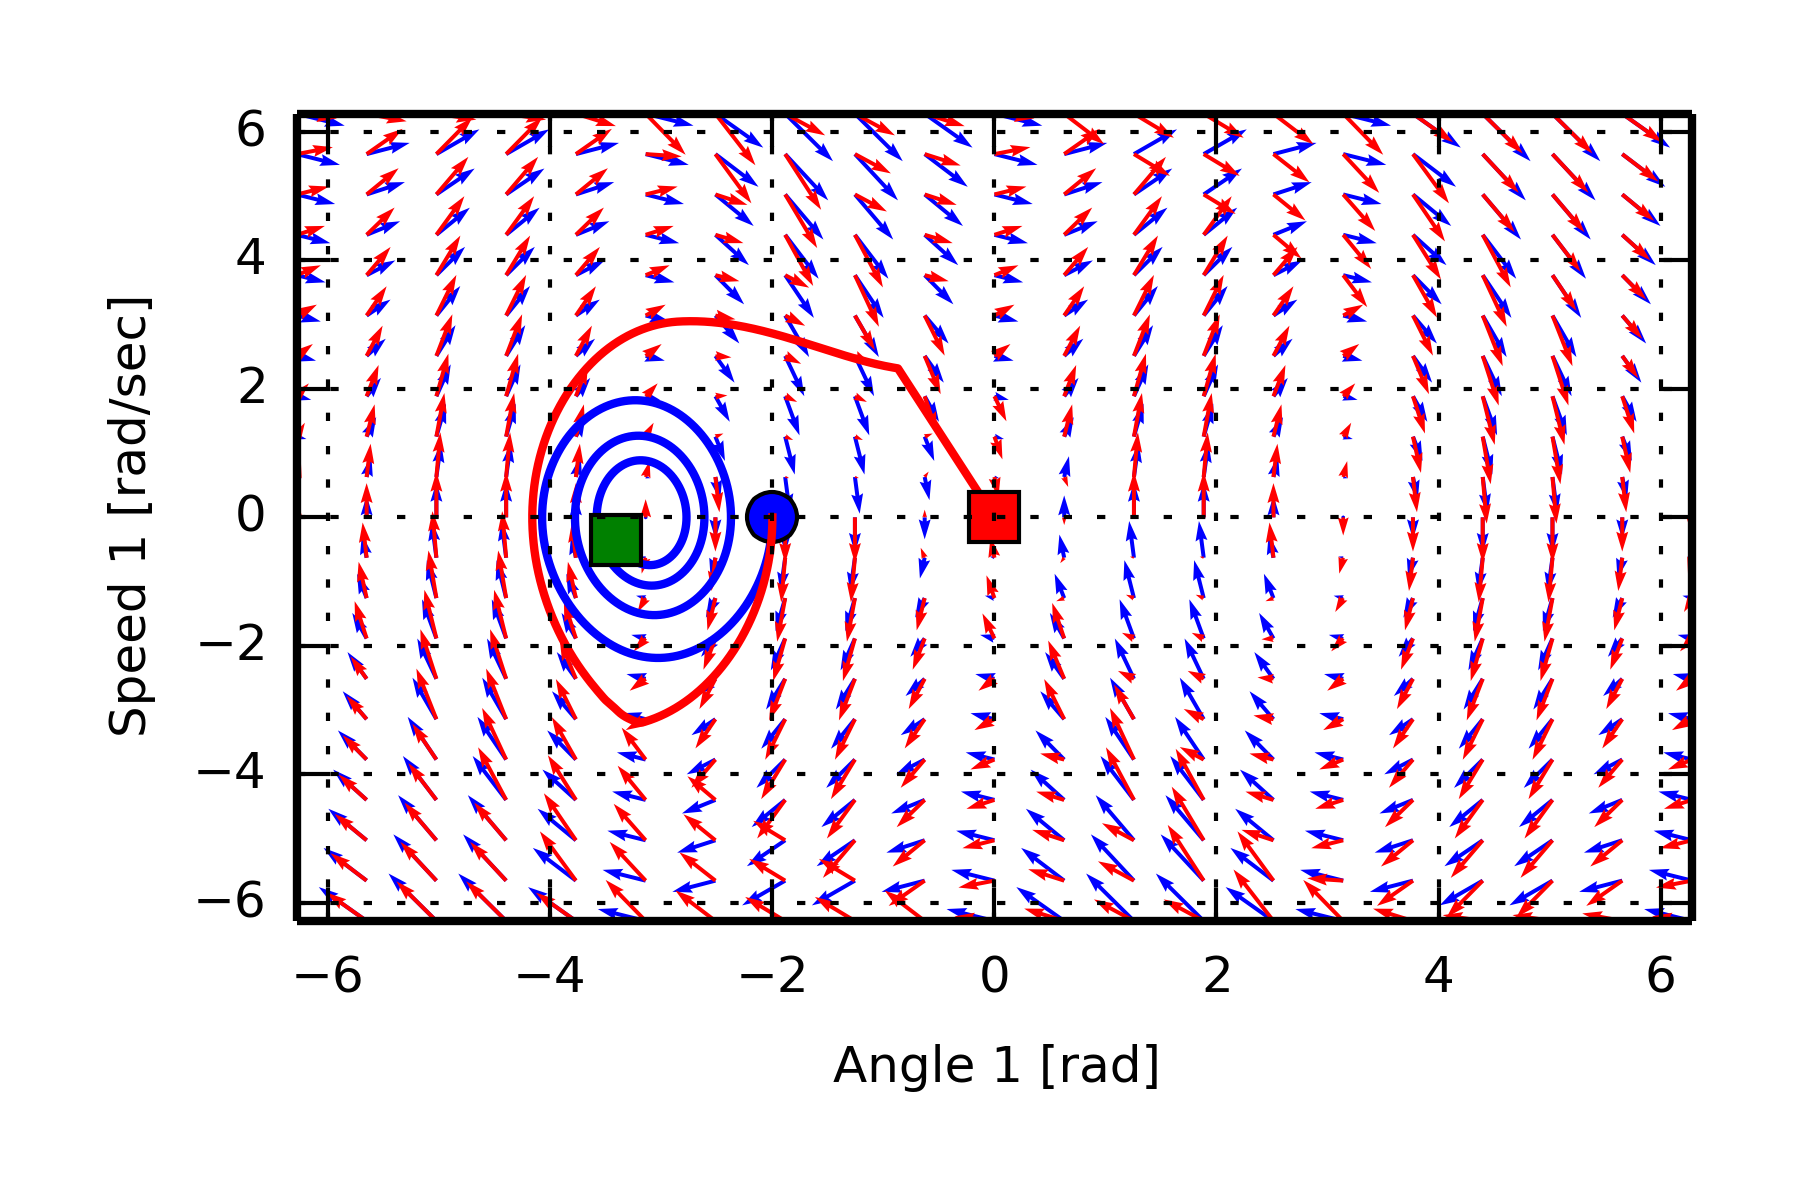
\includegraphics[width=0.48\textwidth]{PP_time.png}
				\label{fig:phase_plane_time2}}
        \subfloat[Quadratic cost]{
				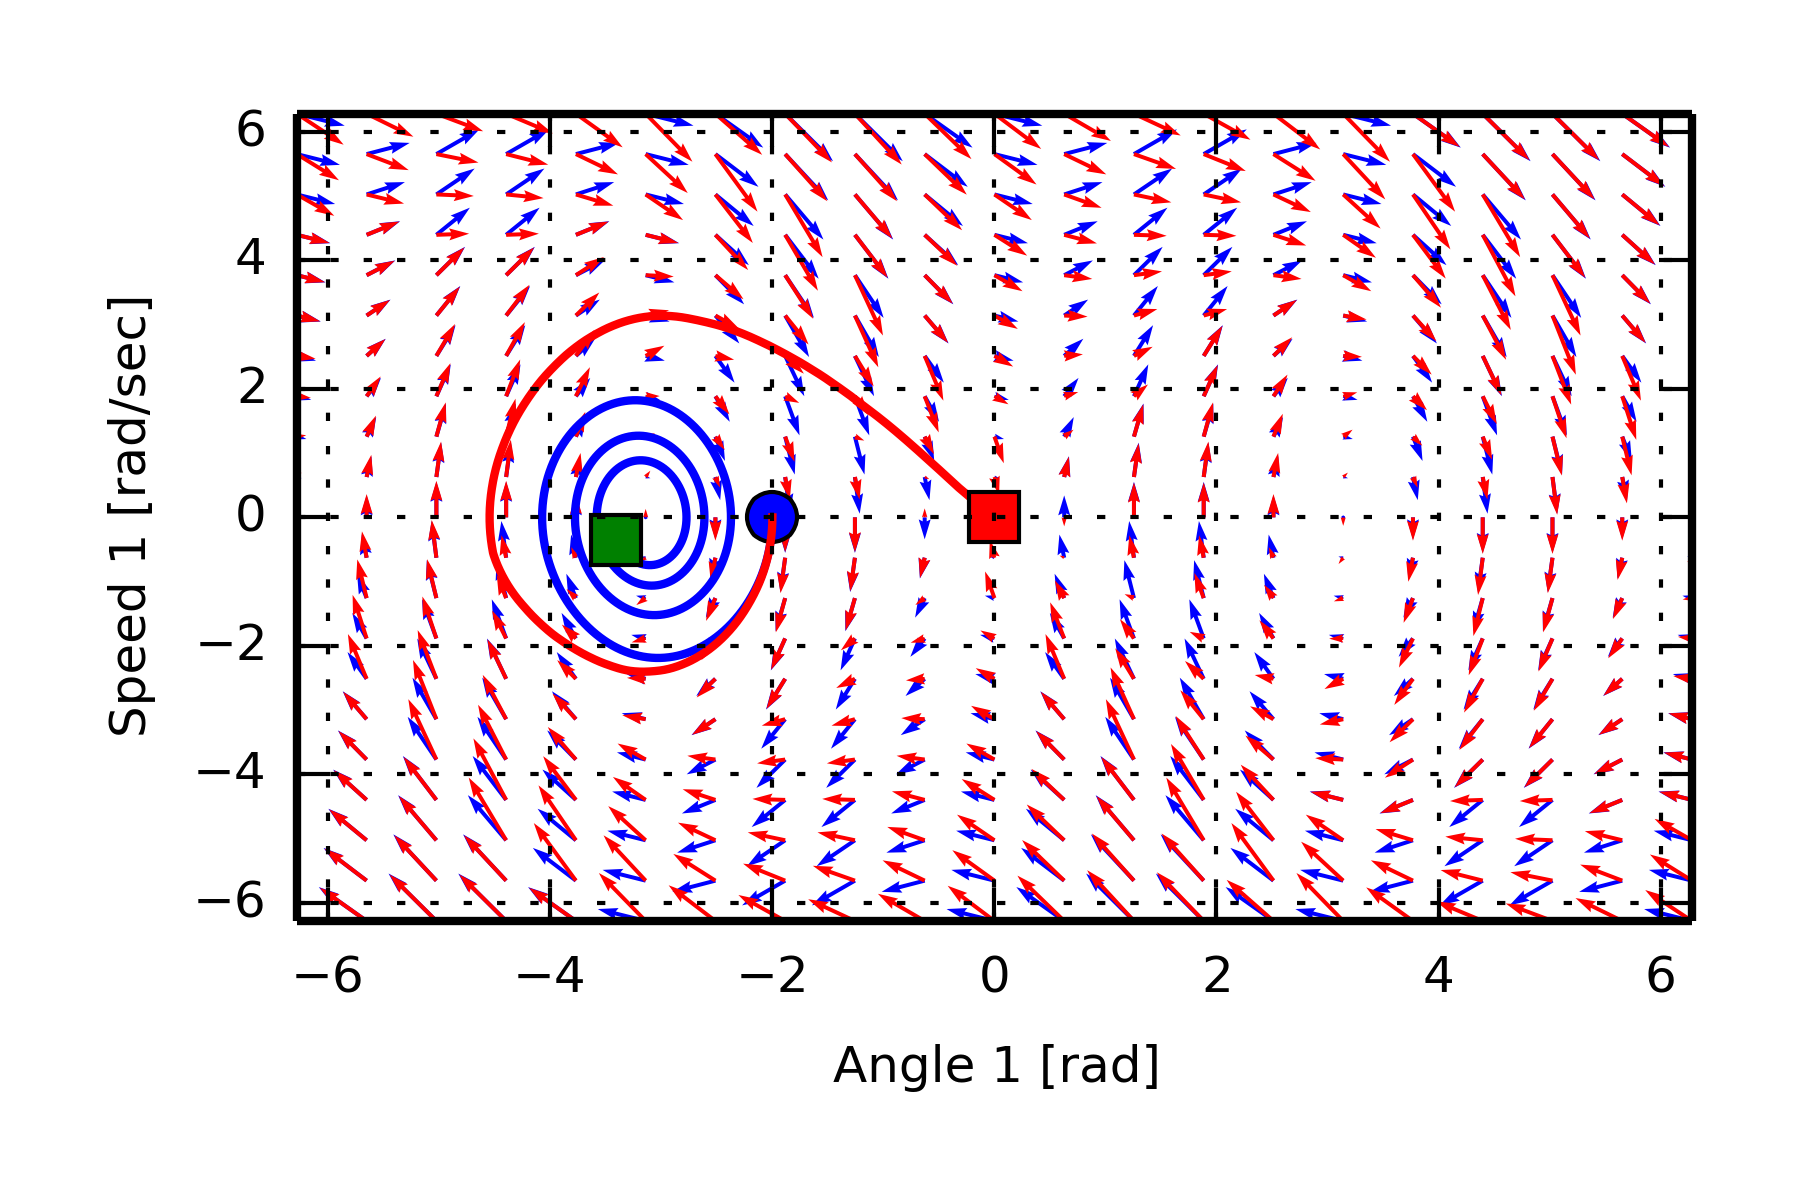
\includegraphics[width=0.48\textwidth]{PP_quadratic.png}
				\label{fig:phase_plane_LQR2}}
        \caption[Closed loop behavior in the phase plane]{Closed loop behavior with the optimal policy illustrated in the phase plane. Two trajectories starting at $q=-2$ are illustrated, blue is open-loop, red is closed loop}\label{fig:phase_plane2}
\end{figure}

For both cost functions the optimal policy for the discrete gear-ratio mode $k$ is quite complex. This illustrates that optimal solutions for this type non-linear hybrid system representative of robotic systems are not trivial, even for a single axis. One observation regarding the gear-ratio selection policy, is that the larger second gear-ratio is used often in situation where the robot needs to be drastically deviated from its natural motion, and the small second gear-ratio is used when the controller let the robot move in the natural direction. This connects back with the idea of attenuating the load-dynamics, with a large gear-ratio when it is advantageous, or leveraging the load-dynamics, with a small gear-ratio when the natural motion is advantageous. 



\subsection{Advanced dynamic programming techniques}

Value iteration is a powerful tool, but computations are intractable for high-dimensional systems. However, there exist many approximate techniques that can be used; approximate dynamic programming is also known as reinforcement learning. The approach proposed in this section, of formulating the control of hybrid robot as a stochastic shortest path problem, could thus be used in conjunction with many approach derived in the field of artificial intelligence such as Q-learning. However, the problem of approximating the cost-to-go, the state-space or the policies in a lower dimensional space, to make computation tractable, is not trivial for non-linear robotic system.


%%%%%%%%%%%%%%%%%%%%%%%%%%%%%%%%%%%%%%%%%%%%%%%%%%%%%%%%%%%%%%%%%%%%%%%%%%%%%%%%%%%%%%%%%%%%%%%%%%%%%%%%%%%%%%%%%%%%%%%%%%%%%%%%%
\newpage
\section{Simulation Results}
\label{sec:shift_sim}


\subsection{Model-based approach}

Here, the advantages of dynamically changing the gear-ratios, using the R* computed torque controller, are illustrated using simulations of two robots: first a 1-DoF pendulum, then a 3-DoF arm. Both robots are considered having VGA with two possible gear-ratios: 1:1 or 1:10. Reference low-torque trajectories to reach target positions are computed with a RRT algorithm. 
%
The first simulated experiment uses a single-axis inverted pendulum equipped with a VGA, see Fig. \ref{fig:vi_sys2}, with the task of reaching the up-right position starting at the bottom. Fig. \ref{fig:sim1} shows the robot tracking the reference low-torque trajectory, where at first the robot accumulates energy, using the 1:1 gear-ratio, and then finishes the motion using the 1:10 gear-ratio. When the gravitational forces are pushing advantageously toward the trajectory the controller select the 1:1 gear-ratio, but when it is advantageous to fight the intrinsic actuator dynamics instead, the 1:10 gear-ratio is selected. This can be seen by comparing the trajectory to natural phase plane vectors as illustrated by Fig. \ref{fig:pps}.
%
\begin{figure}[htp]
	\centering
		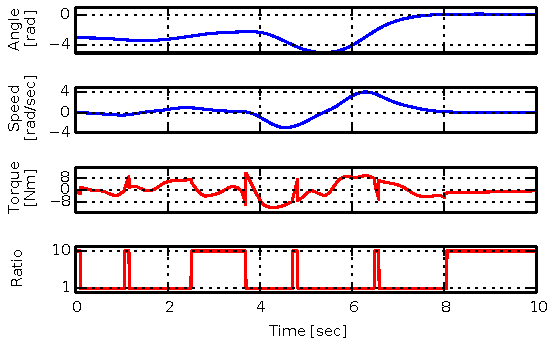
\includegraphics[width=0.90\textwidth]{sim1.pdf}
	\caption{1-DoF robot simulation: states and inputs trajectory}
	\label{fig:sim1}
\end{figure}
%
%
\begin{figure}[htp]
				\vspace{-10pt}
        \centering
				\subfloat[ Reduction ratio $R$=1 ]{ %extrinsic dynamics
				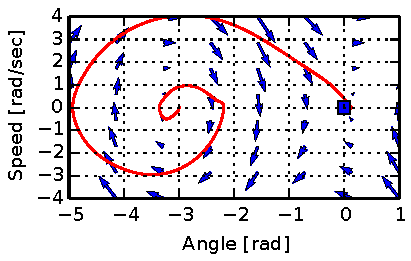
\includegraphics[width=0.45\textwidth]{simpp1.pdf}
				\label{fig:pp1s}}
        \subfloat[Reduction ratio $R$=10 ]{ % intrinsic dynamics
				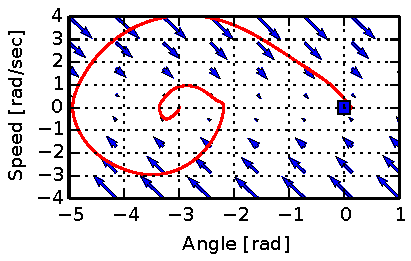
\includegraphics[width=0.45\textwidth]{simpp2.pdf}
				\label{fig:pp2s}}
        \caption{Trajectory superposed with natural dynamics vectors}
				\label{fig:pps}
\end{figure}

%\begin{figure}[htp]
	%\centering
		%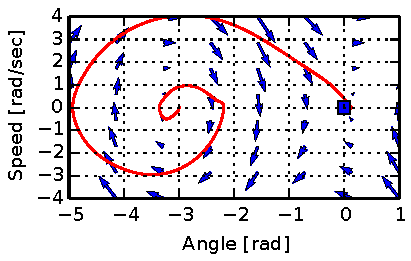
\includegraphics[width=0.38\textwidth]{simpp1.pdf}
	%\caption{Trajectory superposed with natural dynamics vectors with R=1}
	%\label{fig:simpp1}
%\end{figure}
%
%\begin{figure}[htp]
	%\centering
		%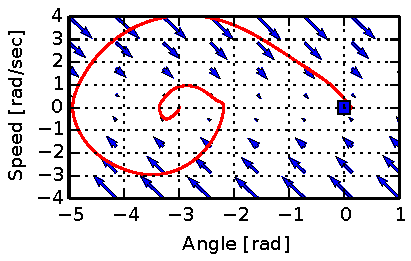
\includegraphics[width=0.38\textwidth]{simpp2.pdf}
	%\caption{Trajectory superposed with natural dynamics vectors with R=10}
	%\label{fig:simpp2}
%\end{figure}

In the second experiment, a 3-DoF manipulator is tasked with going from configuration A to configuration B with the 3D trajectory shown at Fig. \ref{fig:3d_traj}. For this robot the controller is actively selecting the best gear-ratios matrix $R_k$ out of the possible $2^3=8$ options. Fig. \ref{fig:3d_u} shows the control inputs activity. During the initial falling-down phase, at around $t=1$, the robot is using 1:1 gear-ratios for all actuators, leveraging gravitational torques. In contrast, during the final lifting phase, at around $t=6$, the robot is using 1:10 gear-ratios for all actuators. 
%
%
%
\begin{figure}[htp]
	\centering
		%\includegraphics[width=0.45\textwidth]{3dtraj.jpg}
		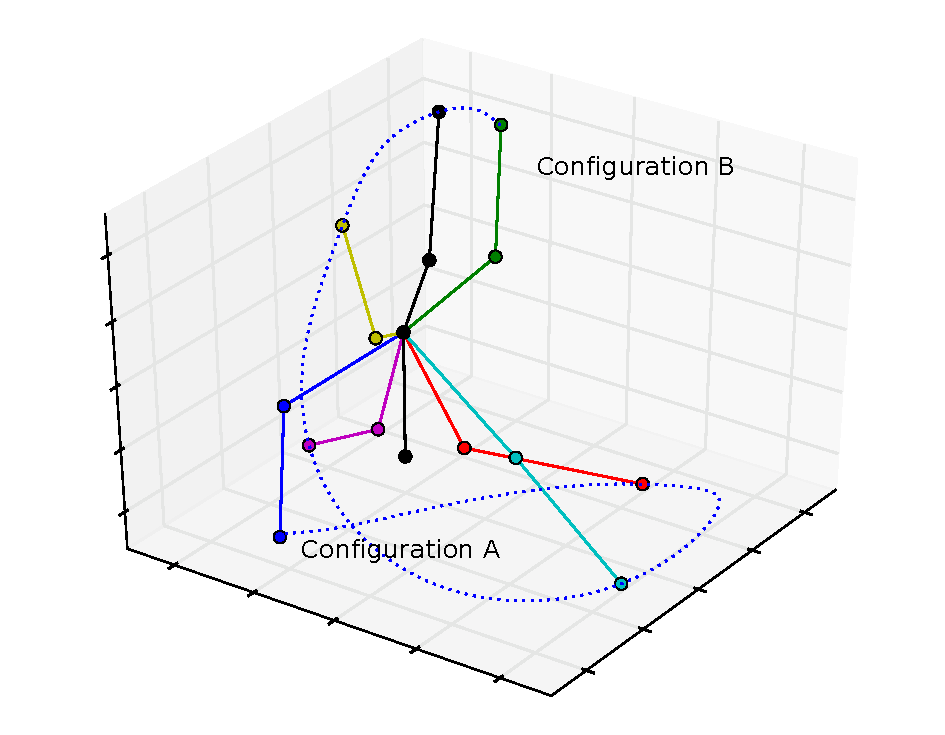
\includegraphics[width=0.75\textwidth]{3d_traj.pdf}
	\caption{ 3-DoF robot simulation: 3D trajectory }
	\label{fig:3d_traj}
\end{figure}
%
%\begin{figure}[htp]
	%\centering
		%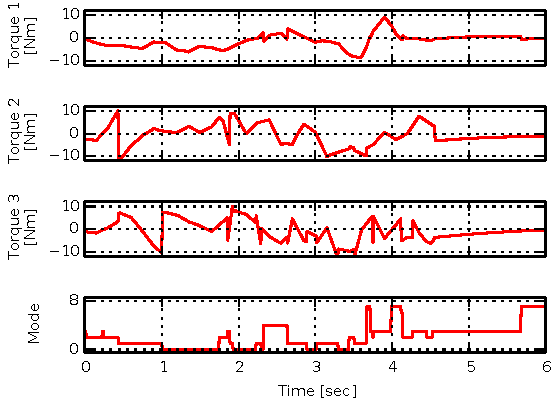
\includegraphics[width=0.40\textwidth]{u_no4.pdf}
	%\caption{ 3-DoF robot simulation: control inputs trajectory where \textit{Mode} represent the index of the selected gear-ratio matrix }
	%\label{fig:3d_u}
%\end{figure}
%
\begin{figure}[htp]
	\centering
		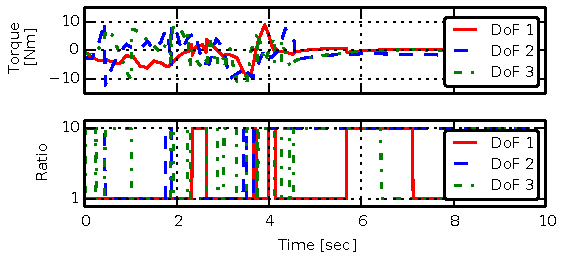
\includegraphics[width=0.75\textwidth]{3d_u.pdf}
	\caption{ 3-DoF robot simulation: control inputs trajectories}
	\label{fig:3d_u}
\end{figure}
%%
%

\subsection{Comparison to fixed-gear performance}

To evaluate the performance gain of actively changing the gear-ratio, simulations with fixed gear-ratios are conducted where a regular computed torque controller tracks the same trajectories. Results are summarized in Table \ref{tab:MaximumTorqueComparison}, in terms of maximum absolute torque, which relates to the required size and weight of motors, and integral of torque squared, which relates to power consumption. Active gear-ratios selection is found to greatly improve both metrics, especially for the 3-DoF robot trajectory where the arm must both achieve high-speeds and also sustain a constant gravitational load at the final configuration. Note that in those simulations high-velocity with 1:10 reductions is inhibited by friction in the motors, no maximum rotor velocity is enforced. For the 3-DoF trajectory, active gear-shifting is found to reduce the maximum torque required by a factor two and the integral of the torque square by a factor 10, compared to any of the fixed-gear options. Those results show the potential of using variable gear-ratio transmissions for huge improvements in terms of actuator size and power consumption. Moreover, here in the simulations, the load was always the same manipulator in different dynamic situations. If the load dynamics is radically changing because of different contact situations with the environment, the performance gain of changing the gear-ratios could be even greater. 
%
\begin{table}[htp]
	\centering
		\caption{Required torque comparison}
		\begin{tabular}{ c c c c }
		\hline
		     & Fixed gear & Fixed gear & Active gearshifting \\
			& 1:1 &  1:10 &  1:1 or 1:10 \\
		\hline \hline
		\multicolumn{4}{c}{ Max Absolute Torque [Nm] } \\
		\hline \hline
		1-link robot  & 15 & 88 & 12 \\	
		3-link robot  & 24 & 42 & 12 \\	
		\hline \hline
		\multicolumn{4}{c}{ Torque squared integral $\int{ ( \vec{\tau}^T \vec{\tau} ) dt }$ } \\
		\hline \hline
		1-link robot  & 377  & 8133 & 226  \\	
		3-link robot  & 2774 & 3617 & 295  \\	
		\hline \hline
		\end{tabular}
	\label{tab:MaximumTorqueComparison}
\end{table}
%

\subsection{Comparison to Value Iteration}

For low-dimensional systems, numerical results obtained with the value iteration algorithm, when discretization is very fine, can almost be seen as a ground truth for the optimal trajectory and optimal global feedback policy. It is thus interesting to compared the model-based approach (RRT planning + R* Computed Torque) to a solution obtained with value iteration, to evaluate how far from the global optimum the model-based control scheme is in some situations. Fig. \ref{fig:vs} shows side-by-side results for a pendulum swing-up task. The trajectory behavior of both solutions is roughly similar, both solutions do a pumping motion to accumulate kinetic energy. The R* Computed Torque controller however apply torques more aggressively, to track the reference trajectory generated by the RRT algorithm which is a rough feasible but un-optimized solution. In term of integral of torque-squared for the whole trajectory, the value iteration solution leads to 72 $\left(Nm\right)^2 \times sec$, compare to 180 $\left(Nm\right)^2 \times sec$ for the RRT with R* computed torque solution.

It is interesting that the model based approach can find a solution with a trajectory and a gear-shifting pattern almost identical to the optimal solution found using value iteration. However, the main drawback is the rough reference trajectory, which as a lot of discontinuities (un-bounded jerk) because the RRT algorithm use a discrete version of the world. A possible approach to alleviate this would be and intermediary step: smoothing out the reference trajectory with a local optimization before it is sent to the R* Computed Controller. By using the RRT trajectory solution as initial conditions and also the gear shift sequence solution, a local optimization would now be much easier to conduct. Quadratic programming algorithms could then be used efficiently to fine tune the reference trajectory solution.

\begin{figure}[H]
				%\vspace{-10pt}
        \centering
				\subfloat[Value Iteration]{ 
				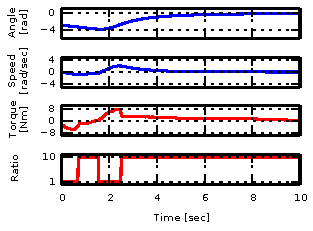
\includegraphics[width=0.50\textwidth]{vs_vi.pdf} }
				%\hspace{-5pt}
				\subfloat[RRT with R* Computed Torque]{ 
				\includegraphics[width=0.50\textwidth]{vs_rrt.pdf} }
        \caption{Model based approach compared to Value Iteration}
				\label{fig:vs}
\end{figure}


\subsection{Fast gear-shifting inhibition}

In the simulations presented so-far, fast gear-shifts were not inhibited by any of the proposed fast-switching inhibiting schemes. Fig. \ref{fig:ChatteringComparaison} shows simulation results, illustrating the gear-ratio command, for the same situation but with three different controllers. 
%
\begin{figure}[htp]
	\centering
		\includegraphics[width=0.90\textwidth]{chattering_compared.pdf}
	\caption{Fast gear-shifting inhibition}
	\label{fig:ChatteringComparaison}
\end{figure}

This figure shows that the hysteresis scheme is not necessary an improvement over the point-by-point gear-ratio selection, since for the gear-shift at $t=1.8$, it would have been better to avoid it completely. The Rollout approach is shown more successful at filtering-out high-frequency switching. Furthermore, another interesting advantageous side effect is observed: with the Rollout approach, the first gear-shift is commanded slightly in advance. This can be advantageous when controlling a real system where the gear-shift process is executed with a delay: the simulation can model this delay and the controller can react in advance accordingly.



%%%%%%%%%%%%%%%%%%%%%%%%%%%%%%%%%%%%%%%%%%%%%%%%%%%%%%%%%%%%%%%%%%%%%%%%%%%%%%%%%%%%%%%%%%%%%%%%%%%%%%%%%%%%%%%%%%%%%%%%%%%%%%%%%

\newpage
\section{Experiments Results}
\label{sec:shift_exp}

This section presents experimental results, focusing on the high-level control aspect, obtained with the experimental DSDM-arm presented in Chapter \ref{sec:ExperimentalValidation}.

\subsection{R* Computed Torque controller and RRT trajectory}

First a trajectory following experiment using only the wrist joint of the robot is presented. A 1.5 Kg load is mounted on the end-effector, and the task is to bring it from the bottom position ($q=-\pi$) to the up-right position ($q=0$) using as little torques as possible. This corresponds to the inverted pendulum swing-up problem. An RRT trajectory planning algorithm is used to search for a feasible low torque trajectory reaching the goal, see Fig. \ref{fig:exp_rrt}. Then the R* Computed Torque Controller is used to track the reference trajectory. The experimental results are shown in Fig. \ref{fig:exp_traj}.
%
\begin{figure}[htp]
	\centering
		\includegraphics[width=0.75\textwidth]{rrt_fig.pdf}
	\caption{RRT algorithm searching for a low torque solution}
	\label{fig:exp_rrt}
\end{figure}
%
\begin{figure}[htp]
	\centering
		\includegraphics[width=0.75\textwidth]{exp_fig3.pdf}
	\caption{Experimental trajectory and control inputs}
	\label{fig:exp_traj}
	\vspace{-10pt}
\end{figure}
%
Results show that the robot is using its 1:23 gear-ratio to accumulate kinetic energy by swinging the arm link back and forth. Also the R* controller selects the 1:474 gear-ratio automatically to attenuate the load dynamics, when the actuator has to force the robot to stay with the trajectory.  Interestingly, the reference trajectory was planned so the robot would accumulate enough kinetic energy to swing straight up with the last swing. However, in the experiment, the dissipative forces are greater than anticipated by the planner, and the last swing is too small (the robot almost stop at $q=-0.9$ at $t=2.6$ in Fig. \ref{fig:exp_traj}). Then, the R* controller automatically engage the large 1:474 gear-ratio, to continue converging on the desired trajectory with much smaller torques than those required if keeping using the 1:23 gear-ratio in this situation (no momentum and a large gravitational force to overpower). This illustrates that including the gear-ratio selection in the feedback loop also increases the robustness of the system. Without the 1:474 gear-ratio option, tracking would have failed as the computed torque with 1:23 in this situation was greater than the maximum allowable motor torque.


\subsection{R* Sliding Mode controller}

Fig. \ref{fig:rob} shows four additional experiments with the wrist demonstrating how disturbance rejection can be improved by using the  R* Sliding Mode controller. Here the controller is only given a simple fixed point-target in all cases. First, when a low uncertainty bound is given to the controller, the robot can reach its target when unloaded (a) but failed when an unknown (to the controller) 0.4 Kg load is added to the end-effector (b). However, when a larger uncertainty bound is given, the robot can reach its target in both cases, unloaded (c) and loaded (d). 

\begin{figure}[htp]
				%\vspace{-10pt}
        \centering
				\hspace{-10pt}
				\subfloat[]{ % intrinsic dynamics
				\includegraphics[width=0.30\textwidth]{fig16a.pdf} }
				\hspace{-5pt}
        \subfloat[]{ % intrinsic dynamics
				\includegraphics[width=0.20\textwidth]{fig16b.pdf} }
				\hspace{-5pt}
				\subfloat[]{ % intrinsic dynamics
				\includegraphics[width=0.20\textwidth]{fig16c.pdf} }
				\hspace{-5pt}
				\subfloat[]{ % intrinsic dynamics
				\includegraphics[width=0.20\textwidth]{fig16d.pdf} }
        \caption{Experiments with Sliding Mode version of the R* controller }
				\label{fig:rob}
\end{figure}

Note that the discontinuous torque required to guarantee convergence despite disturbances is bigger for the case when the disturbance bound is increased, and is greatly reduced when using the large gear-ratio at low speeds (since the required discontinuous gain is inversely proportional to the gear-ratio). In a practical implementation, smoothing techniques should be implemented to avoid exciting the unmodeled high-frequency modes with the torque chattering.

\subsection{2-DoF experiments}

Fig. \ref{fig:exp_traj_2dof_x} and Fig. \ref{fig:exp_traj_2dof_u} show an experiment using 2-DoF, the wrist joint and the elbow joint of the DSDM-Arm. The goal is a fixed joint configuration, and the R* Sliding Mode controller, including the Rollout gear-selection scheme, is used. Results shows success in tracking the goal for both DoF. Also, it is possible to observe that the downshift at $t=2.6$ allows for a drastic reduction of the necessary discontinuous torque to guarantee convergence, illustrating the advantage of isolating the motor from the external load with a large reduction ratio in some situations.

%
\begin{figure}[htp]
	\centering
		\includegraphics[width=0.85\textwidth]{2dof_test3_x.pdf}
	\caption{R* Sliding Mode controller tracking a target with 2 DoF: trajectory}
	\label{fig:exp_traj_2dof_x}
	%\vspace{-10pt}
\end{figure}
%

%
\begin{figure}[htp]
	\centering
		\includegraphics[width=0.85\textwidth]{2dof_test3_u.pdf}
	\caption{R* Sliding Mode controller tracking a target with 2 DoF: control inputs}
	\label{fig:exp_traj_2dof_u}
	%\vspace{-10pt}
\end{figure}
%




%%%%%%%%%%%%%%%%%%%%%%%%%%%%%%%%%%%%%%%%%%%%%%%%%%%%%%%%%%%%%%%%%%%%%%%%%%%%%%%%%

\newpage

\section{Summary}

In this Chapter, feedback laws for controlling both the torques and gear-ratios of robotic systems equipped with variable transmissions are proposed. A simple dynamic model is proposed, and analytical solutions are derived for the optimal gear-ratios on a known trajectory. The approach is extended to trajectory tracking control schemes (R* Computed Torque and R* Sliding Mode), which can guarantee convergence on a reference trajectory and execute locally optimal gear-ratios based on state feedback. An approach (Rollout gear-selection) is also proposed to inhibit fast gear-shifting by optimizing over a receding time-horizon. An alternative computational technique (Value iteration) is also explored to generate global control policies for both torque and gear-ratios for simple systems. Simulation and experimental results demonstrate the effectiveness of the proposed controllers.

\section{Potential directions of further development}

Here are a few possible axis of further development: 

\begin{itemize}
		\item Improving the proposed control approaches:
		\begin{itemize}
			\item Using reinforcement learning to learn good gear-selection policies;
			\item Explore adaptive controllers;
			\item Decentralizing the gear-ratios selection decisions.
		\end{itemize}
		\item Explore more specific applications:
		\begin{itemize}
			\item Legged locomotion or manipulation including contacts;
			\item Interaction tasks requiring a wide range of impedance.
		\end{itemize}
		\item Open research questions not addressed:
		\begin{itemize}
			\item Controlling under-actuated robots using VGA;
			\item Efficient trajectory optimization for robots using VGA.
		\end{itemize}
\end{itemize}